\documentclass[%
  aspectratio=169,
  9pt,
  USenglish,
  titlegraphic, % store custom image to .images/titlegraphic
  affiliationintitlepagehead,
  progressbar,
%   affiliation,
]{beamer}

\usetheme{TUM}

\usepackage{tikz}  
\usepackage{tikz-3dplot} 
\usepackage{graphicx}
\usepackage{media9}
\usetikzlibrary{positioning}

\usepackage{amsmath}
\usepackage{booktabs}

% change the camera position
\tdplotsetmaincoords{45}{135}

\usepackage{tabularx}



\usepackage{animate}

\usepackage{pgfmath}
\newcommand\randmin{}
\newcommand\randmax{}
\newcommand\randmultof{}
\newcommand\setrand[4]%
{\def\randmin{#1}%
	\def\randmax{#2}%
	\def\randmultof{#3}%
	\pgfmathsetseed{#4}%
}
\newcommand\nextrand
{\pgfmathparse{int(int((rnd*(\randmax-\randmin+1)+\randmin)/\randmultof)*\randmultof)}%
	\xdef\thisrand{\pgfmathresult}%
}

%\usepackage[backend=biber]{biblatex}
%\addbibresource{bib/references.bib}

\newcommand{\wave}{
	\begin{tikzpicture}[xscale=.03,yscale=.1]
	\draw[-,fill=white] plot[domain=0:10*pi,smooth] (\x,{sin(\x r)});
	\end{tikzpicture}
}


\newcommand{\domain}[4]{
	%% spatial,spectral,temporal
	\draw[fill=#4, opacity=.2] (#1,0,0) -- (0,#2,0) -- (0,0,#3) -- (#1,0,0);
}


\newcommand{\radarwave}{
	\begin{tikzpicture}[xscale=.1,yscale=.2]
	\draw[-,fill=white] plot[domain=0:5*pi,smooth] (\x,{sin(\x r)});
	\end{tikzpicture}
}


\newcommand{\earth}{
	\begin{tikzpicture}[baseline=-.25em, inner sep=0]
	\node{
\includegraphics[width=8mm]{images/icons/earth}};
	\end{tikzpicture}
}

\newcommand{\sat}{
	\begin{tikzpicture}[baseline=-.25em, inner sep=0, remember picture]
	\node(sat)[rotate=270,anchor=center]{
\includegraphics[width=8mm]{images/icons/sat2}};
	\end{tikzpicture}
}


\usepackage[capitalize]{cleveref}
\usepackage[square,sort,comma,numbers]{natbib}

%% this hack seems to be nececessary due to incompatibilities of cvpr template and tikz... -> https://tex.stackexchange.com/questions/398223/tikz-gives-error-command-everyshipouthook-already-defined
%\makeatletter
%\@namedef{ver@everyshi.sty}{}
%\makeatother
%% hackend

\usepackage{tikz}
\usepackage{pgfplots}
\usetikzlibrary{positioning, calc,arrows,arrows.meta, fit}
%\usetikzlibrary{arrows.meta,calc,decorations.markings,math,arrows.meta}
\usepgfplotslibrary{groupplots}
\usepgfplotslibrary{fillbetween}
\usepgfplotslibrary{statistics} % provides boxplots
\usepackage{xfrac}

\newcommand{\tp}{tp}
\newcommand{\tn}{tn}
\newcommand{\fp}{fp}
\newcommand{\fn}{fn}


\usepackage{tumcolors}
\usepackage{tummath}
\newcommand{\yhat}{\hat{\V{y}}}
\newcommand{\ycorrect}{\hat{y}^+}
\newcommand{\thetadelta}{\V{\Theta}_\delta}
\newcommand{\biasdelta}{b_\delta}
\newcommand{\biasclass}{\V{b}_\text{c}}
\newcommand{\thetaclass}{\V{\Theta}_\text{c}}
\newcommand{\thetafeat}{\V{\Theta}_\text{feat}}
\newcommand{\fclass}{f_\text{c}}
\newcommand{\fdelta}{f_\delta}
\newcommand{\ffeat}{f_\text{feat}}
\newcommand{\f}{f}

\newcommand{\rvtime}{T_c} 
\newcommand{\xuptot}{\M{X}_{\rightarrow t}} 
\newcommand{\deltauptot}{\delta_{\rightarrow t}} 
\newcommand{\tstop}{\ensuremath{t_\text{stop}}}
\newcommand{\meantstop}{\ensuremath{\bar{t}_\text{stop}}}
\usepackage[super]{nth}
\usepackage{mathtools}

\definecolor{evalcolor}{HTML}{3F3F3F}
\definecolor{traincolor}{HTML}{B98951}
\definecolor{validcolor}{HTML}{3F4BBE}

\definecolor{fdlcolor}{HTML}{142737}

\usepackage{multimedia}

\colorlet{colortrain}{tumblue}
\colorlet{colorinfer}{tumblack}

\colorlet{earlinesscolor}{tumblue}
\colorlet{accuracycolor}{tumorange}

\colorlet{stdcolor}{tumbluelight}
\colorlet{mediancolor}{tumorange}
\colorlet{meancolor}{tumblue}

\colorlet{b1color}{tumdiagramaubergine}
\colorlet{b2color}{tumdiagramnavyblue}
\colorlet{b3color}{tumdiagramturquoise}
\colorlet{b4color}{tumdiagramgreen}
\colorlet{b5color}{tumdiagramlimegreen}
\colorlet{b6color}{tumdiagramyellow}
\colorlet{b7color}{tumdiagramsand}
\colorlet{b8color}{tumdiagramredorange}
\colorlet{b8Acolor}{tumdiagramred}
\colorlet{b9color}{tumblack}
\colorlet{b10color}{tumblue}
\colorlet{b11color}{tumdiagramdarkred}
\colorlet{b12color}{tumorange}

% atmospheric bands
\colorlet{b1color}{tumblack}%tumdiagramaubergine
\colorlet{b9color}{tumblack}%tumblack
\colorlet{b10color}{tumblack}%tumblue

%visisble bands
\colorlet{b2color}{tumblue}%tumdiagramnavyblue
\colorlet{b3color}{tumblue}%tumdiagramturquoise
\colorlet{b4color}{tumblue}%tumdiagramgreen

% near infrared bands
\colorlet{b5color}{tumdiagramred}%tumdiagramlimegreen
\colorlet{b6color}{tumdiagramred}%tumdiagramyellow
\colorlet{b7color}{tumdiagramred}%tumdiagramsand
\colorlet{b8color}{tumdiagramred}%tumdiagramredorange
\colorlet{b8Acolor}{tumdiagramred}%tumdiagramred

% SWIR bands
\colorlet{b11color}{tumorange}%tumdiagramdarkred
\colorlet{b12color}{tumorange}%tumorange

\colorlet{epsilon0color}{tumorange}
\colorlet{epsilon1color}{tumblue}
\colorlet{epsilon10color}{tumblack}

\colorlet{gridcolor}{tumblue}
\colorlet{activationcolor}{tumorange}

\colorlet{meadowcolor}{tumbluemedium}
\colorlet{wbarleycolor}{tumbluedark}
\colorlet{corncolor}{tumorange}
\colorlet{wheatcolor}{tumgreen}
\colorlet{sbarleycolor}{tumdiagramred}
\colorlet{clovercolor}{tumdiagramturquoise}
\colorlet{triticalecolor}{tumdiagramsand}

\tikzstyle{rnn}=[draw,circle, inner sep=.1em]
\tikzstyle{norm}=[rounded corners,draw]
\tikzstyle{annotation}=[rounded corners, fill=tumblue!20]
\tikzstyle{annot}=[-Stealth, thick]
\tikzstyle{infer}=[-stealth, shorten >=.0em, shorten <=.0em, colorinfer]
\tikzstyle{loss}=[fill=tumblue!10, rounded corners, font=\small]
\tikzstyle{grad}=[colortrain]

\newcommand{\ptoffset}{\varepsilon}

\tikzstyle{test} = [thick]
\tikzstyle{train} = [thin, dotted]

\usepackage[inline]{enumitem}
\setenumerate{label=(\roman*),itemsep=3pt,topsep=3pt}

\setlength{\belowcaptionskip}{-10pt}


\colorlet{traincolor}{tumbluelight}
\colorlet{validcolor}{tumbluedark}
\colorlet{evalcolor}{tumorange}

\colorlet{forwardcolor}{tumblue}
\colorlet{backwardcolor}{tumorange}

% defaultvalue -> might be replaced later
\colorlet{tensorcolor}{forwardcolor}

\colorlet{classcolor}{tumivory}
\colorlet{encodercolor}{tumblue}
\colorlet{encodercolor}{tumblue}
\colorlet{colorblue}{tumblue}
\colorlet{colororange}{tumorange}

\colorlet{colorclassone}{tumblue}
\colorlet{colorclasstwo}{tumblack}
\colorlet{colorclassthree}{tumorange}
\colorlet{colorclassfour}{tumgray}

\colorlet{frh01color}{tumgray}
\colorlet{frh02color}{tumorange}
\colorlet{frh03color}{tumblue}
\colorlet{frh04color}{tumblack}



%\usepackage{media9}

% notation
\newcommand{\MWeight}{\ensuremath{\M{W}}}
\newcommand{\VBias}{\ensuremath{\V{b}}}
\newcommand{\VInput}{\DataVec}
\newcommand{\VHidden}{\ensuremath{\V{h}}}
\newcommand{\FActivation}{\ensuremath{\sigma}}
\newcommand{\VCellState}{\ensuremath{\V{c}}}
\newcommand{\VForgetGate}{\ensuremath{\V{f}}}
\newcommand{\VModulationGate}{\ensuremath{\V{j}}}
\newcommand{\VInputGate}{\ensuremath{\V{i}}}
\newcommand{\VOutputGate}{\ensuremath{\V{o}}}
\newcommand{\concat}[2]{\left[#1 \parallel #2\right]}


\newcommand{\VResetGate}{\ensuremath{\V{r}}}
\newcommand{\VUpdateGate}{\ensuremath{\V{u}}}


%\usepackage{titlesec}
%\titlespacing{\section}{0pt}{10pt}{3pt}


\usetikzlibrary{3d}
\tikzstyle{perspective3d}=[
x={(0.5cm,0.5cm)}, y={(1cm,0cm)}, z={(0cm,1cm)}]


\usetikzlibrary{spy}

\usetikzlibrary{external,pgfplots.dateplot}

\usepackage[eulergreek]{sansmath}
\pgfplotsset{
	y tick label style={/pgf/number format/.cd,%
		scaled y ticks = false,
		set thousands separator={},
		fixed},
	x tick label style={/pgf/number format/.cd,%
		scaled x ticks = false,
		set decimal separator={,},
		fixed},
	tick label style = {font=\scriptsize\sansmath\sffamily},
	every axis label = {
		font=\scriptsize\sansmath\sffamily},
	every axis/.append style={
		axis lines=left, 
		enlargelimits, 
		thick},
	legend style = {font=\scriptsize\sansmath\sffamily, draw=none, rounded corners=0, fill opacity=.5, text opacity=1},
	label style = {font=\scriptsize\sansmath\sffamily},
	grid style={line width=.1pt, draw=gray!10},
	major grid style={line width=.2pt,draw=tumgraylight},
}

%\let\tempone\itemize
%\let\temptwo\enditemize
%\renewenvironment{itemize}{\tempone\addtolength{\itemsep}{-.5\baselineskip}}{\temptwo}

\tikzstyle{circ} = [circle, draw=white, fill=tumblue, inner sep=1pt]
\newcommand{\fcn}{
	\begin{tikzpicture}[scale=0.2, rotate=0, baseline=-.25em, inner sep=1pt]
	\node[circ](a0) at (0,-1){};
	\node[circ](a1) at (0,0){};
	\node[circ](a2) at (0,1){};
	
	\node[circ](b0) at (1,-0.5){};
	\node[circ](b1) at (1,0.5){};
	
	\draw[-] (a0) -- (b0);
	\draw[-] (a1) -- (b0);
	\draw[-] (a2) -- (b0);
	
	\draw[-] (a0) -- (b1);
	\draw[-] (a1) -- (b1);
	\draw[-] (a2) -- (b1);
	
	\end{tikzpicture}
}

\newcommand{\lfcn}[1]{
	\begin{tikzpicture}[scale=#1, rotate=0, baseline=-.25em, inner sep=1pt]
	\node[circle, draw=white, fill=tumblue, inner sep=3](a0) at (0,-1){};
	\node[circle, draw=white, fill=tumblue,  inner sep=3](a1) at (0,0){};
	\node[circle, draw=white, fill=tumblue,  inner sep=3](a2) at (0,1){};
	
	\node[circle, draw=white, fill=tumblue,  inner sep=3](b0) at (1,-0.5){};
	\node[circle, draw=white, fill=tumblue,  inner sep=3](b1) at (1,0.5){};
	
	\draw[-] (a0) -- (b0);
	\draw[-] (a1) -- (b0);
	\draw[-] (a2) -- (b0);
	
	\draw[-] (a0) -- (b1);
	\draw[-] (a1) -- (b1);
	\draw[-] (a2) -- (b1);
	
	\end{tikzpicture}
}

\newcommand{\hidden}[1]{
	\begin{tikzpicture}[scale=.1, baseline=-.25em]	
	%\draw[step=1.0,black,thin] (0,0) grid (#1,1);
	\foreach \i in {1,...,#1}{
		\node[circle, draw=white, fill=tumbluelight, inner sep=1pt] at (\i,0){};
	}
	\end{tikzpicture}
}

\newcommand{\drawvector}[1]{
	\begin{tikzpicture}[scale=.1, baseline=-.25em]	
	%\draw[step=1.0,black,thin] (0,0) grid (#1,1);
	\foreach \i in {1,...,#1}{
		\node[circ] at (\i,0){};
	}
	\end{tikzpicture}
}

%%%%%%%%%%%
%Coordinate Grid for easier placement of nodes
% \draw (0,1) to[grid with coordinates] (10,7);
%%%%%%%%%%%
\makeatletter
\def\grd@save@target#1{%
	\def\grd@target{#1}}
\def\grd@save@start#1{%
	\def\grd@start{#1}}
\tikzset{
	grid with coordinates/.style={
		to path={%
			\pgfextra{%
				\edef\grd@@target{(\tikztotarget)}%
				\tikz@scan@one@point\grd@save@target\grd@@target\relax
				\edef\grd@@start{(\tikztostart)}%
				\tikz@scan@one@point\grd@save@start\grd@@start\relax
				\draw[minor help lines] (\tikztostart) grid (\tikztotarget);
				\draw[major help lines] (\tikztostart) grid (\tikztotarget);
				\grd@start
				\pgfmathsetmacro{\grd@xa}{\the\pgf@x/1cm}
				\pgfmathsetmacro{\grd@ya}{\the\pgf@y/1cm}
				\grd@target
				\pgfmathsetmacro{\grd@xb}{\the\pgf@x/1cm}
				\pgfmathsetmacro{\grd@yb}{\the\pgf@y/1cm}
				\pgfmathsetmacro{\grd@xc}{\grd@xa + \pgfkeysvalueof{/tikz/grid with coordinates/major step}}
				\pgfmathsetmacro{\grd@yc}{\grd@ya + \pgfkeysvalueof{/tikz/grid with coordinates/major step}}
				\foreach \x in {\grd@xa,\grd@xc,...,\grd@xb}
				\node[anchor=north] at (\x,\grd@ya) {\pgfmathprintnumber{\x}};
				\foreach \y in {\grd@ya,\grd@yc,...,\grd@yb}
				\node[anchor=east] at (\grd@xa,\y) {\pgfmathprintnumber{\y}};
			}
		}
	},
	minor help lines/.style={
		help lines,
		step=\pgfkeysvalueof{/tikz/grid with coordinates/minor step}
	},
	major help lines/.style={
		help lines,
		line width=\pgfkeysvalueof{/tikz/grid with coordinates/major line width},
		step=\pgfkeysvalueof{/tikz/grid with coordinates/major step}
	},
	grid with coordinates/.cd,
	minor step/.initial=.2,
	major step/.initial=1,
	major line width/.initial=2pt,
}
\makeatother

\newcommand\tikzmark[1]{
	\tikz[remember picture,overlay] \coordinate (#1);
}
\newcommand\remembername[2]{
	\begin{tikzpicture}[inner sep=0]
		\node(#2){#1};
	\end{tikzpicture}
%	\tikz[remember picture,overlay] \coordinate (#1);
}

\newcommand{\bluebf}[1]{{\color{tumblue}\textbf{#1}}}
\newcommand{\orangebf}[1]{{\color{tumorange}\textbf{#1}}}

\setbeamertemplate{blocks}[rounded][shadow=false]

\title{Learning Vegetation Models from Satellite Data}
\subtitle{L'Information Grandeur Nature (IGN)---getting-in-touch}
\author[M. Rußwurm]{Marc Rußwurm, advised by Dr. rer. nat. Marco Körner}
\institute[TUM]{Technical University of Munich, Germany\\
                Remote Sensing Technology}
\date{July 10th, 2019}

\begin{document}
\begin{frame}[t]
  \titlepage
\end{frame}


{\setbeamercolor{background canvas}{bg=white}
	\begin{frame}[plain]
	\vfill
	\begin{center}
		\Huge\color{black}
		Hi!
		\hspace{2em}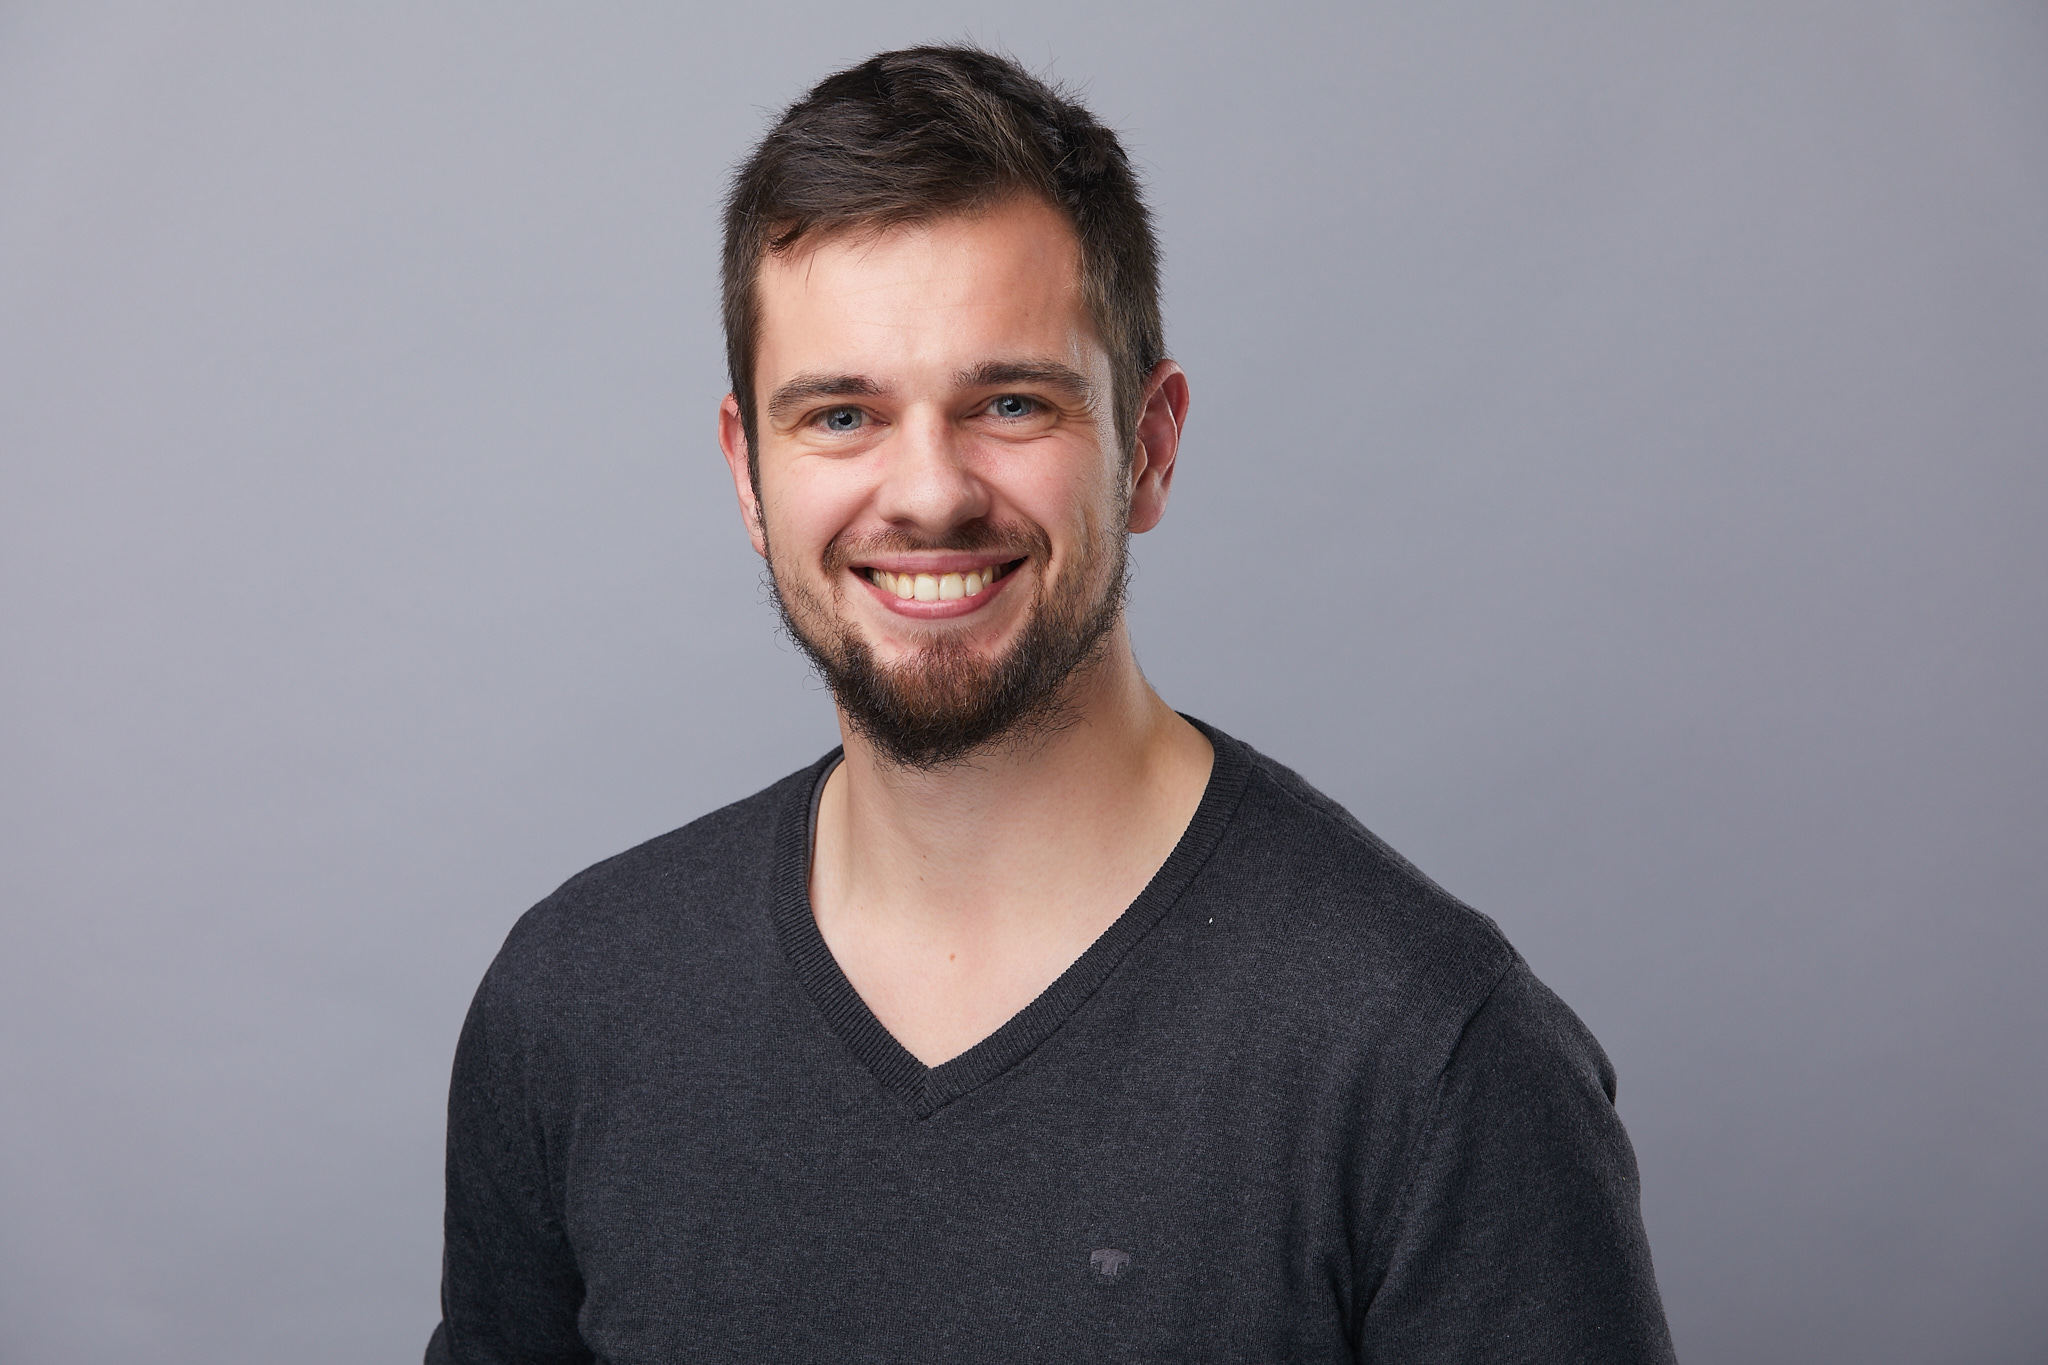
\includegraphics[width=5cm]{images/marc}
		\vspace{2em}
		
		\Large\raggedright
		
		Marc Rußwurm M.Sc. \\
		\vspace{1em}
		PhD Candidate at~
\includegraphics[height=.9em]{images/TUM-white}~Chair of Remote Sensing Technology
	\end{center}
	\vfill
\end{frame}
}


\begin{frame}
\frametitle{Background}

\tikzstyle{event} = [font=\small, text width=3.8cm, rounded corners=2em, inner sep=.7em]
\tikzstyle{date} = [font=\small, fill=white]
%
%\vspace{2em}

\begin{tikzpicture}[xscale=9, yscale=.85]

\visible<1->{\node[anchor=east, label=Earth Observation] at (0,0){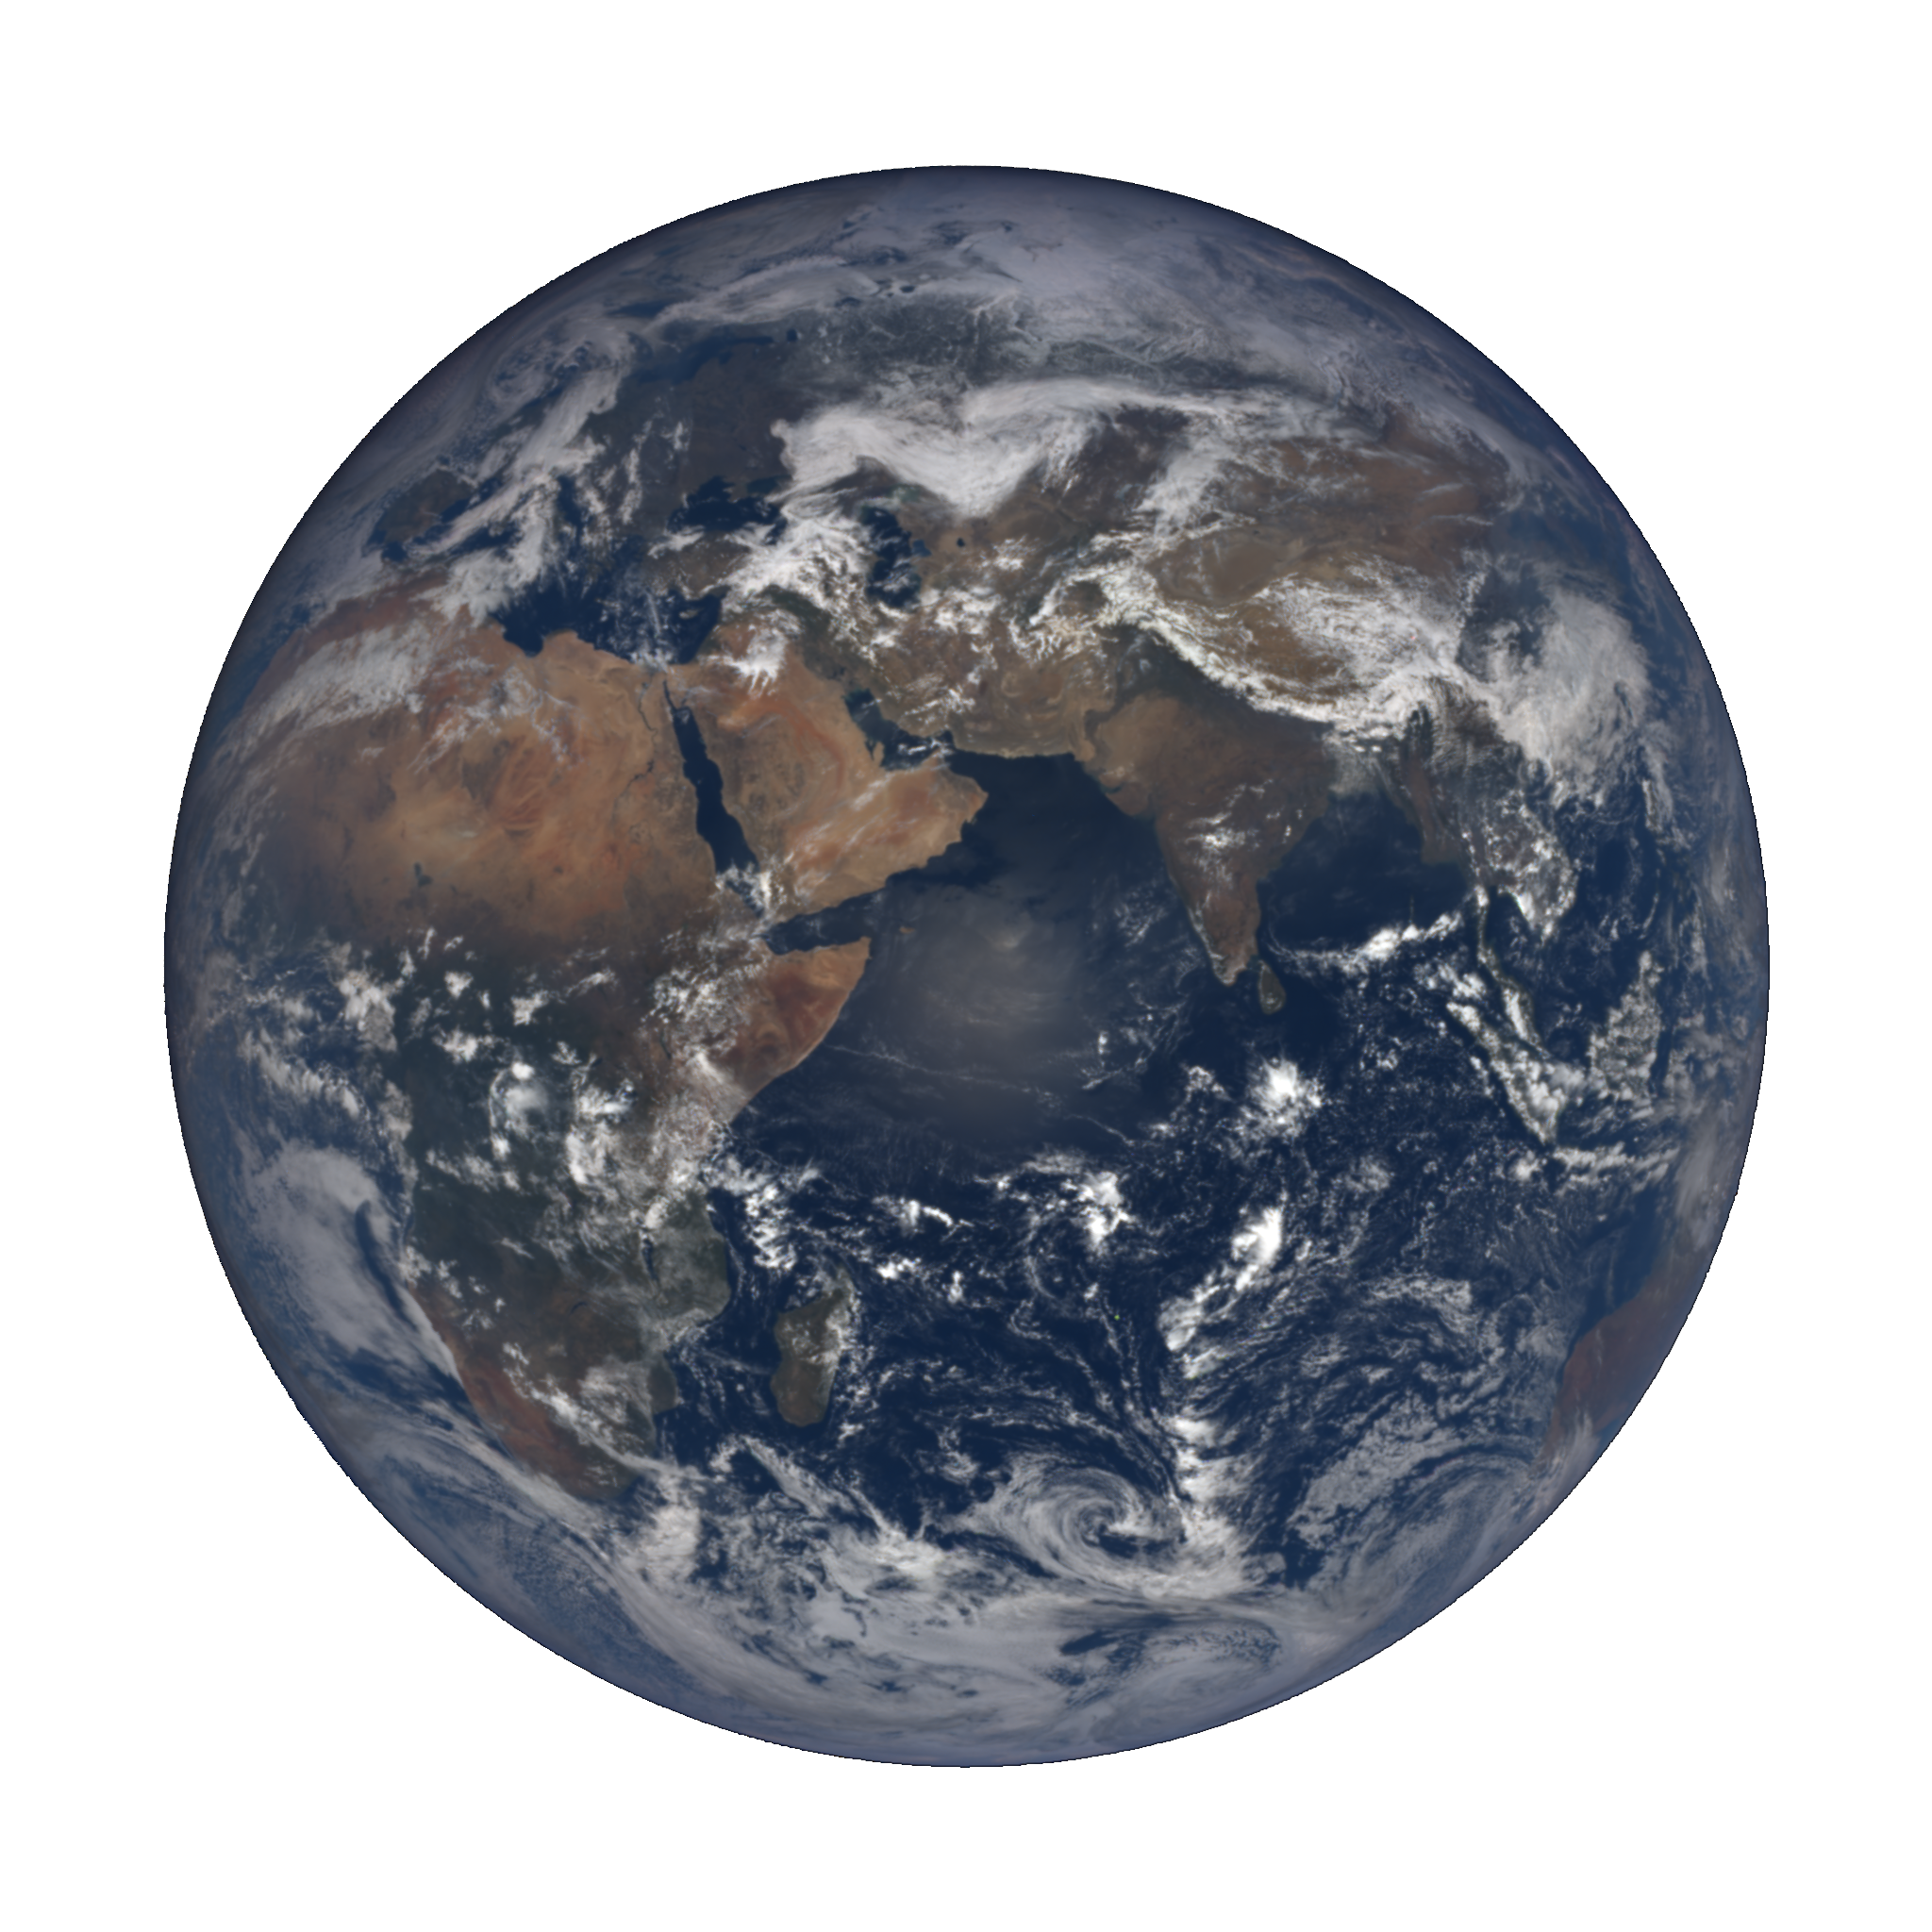
\includegraphics[width=3cm]{images/epicw1}};}
\visible<4->{\node[anchor=west, label=Machine Learning] at (1.1,0){\lfcn{.75}};}

\node[event, fill=tumorange!50] at (.2,1) {2012-2018 \\ \textbf{Bachelor/Master} \\ Geodesy and Geoinformation};

\visible<2->{\node[event, fill=tumbluelight] at (.3,-1) {2014 \\ Interned at University of Otago, NZ. \\ Geodata Visualization};}

\visible<3->{\node[event, fill=tumbluelight] at (.1,-3) {2016 \\ Erasmus-interned at Polish Earth Observation Center \\ \textbf{Opium Poppy Detection}};}

\visible<4->{\node[event, fill=tumorange!50] at (.7,2) {2018-2022 \\ \textbf{PhD} with Supervisor from Computer Vision \\ Multi-temporal Earth Observation};}

\visible<5->{\node[event, fill=tumbluelight] at (.7,-3) {2018 \\ Participant \\ Frontier Developments Lab \\ Disaster Relief with \textbf{CNN data fusion}};}

\visible<6->{\node[event, fill=tumbluelight] at (.8,-.5) {2019 \\ Research Stay IRISA Obelix Lab in France \\ \textbf{Early Classification of Time Series}};}

\end{tikzpicture}

\end{frame}



{\setbeamercolor{background canvas}{bg=black}
	\begin{frame}[plain]
	
	\vfill
	\Huge\color{white}
	\begin{center}
		\begin{columns}
			\column{.5\textwidth}
			\vspace{7em}
			
			\hfill 
			Earth Observation Data
			\column{.5\textwidth}
			
			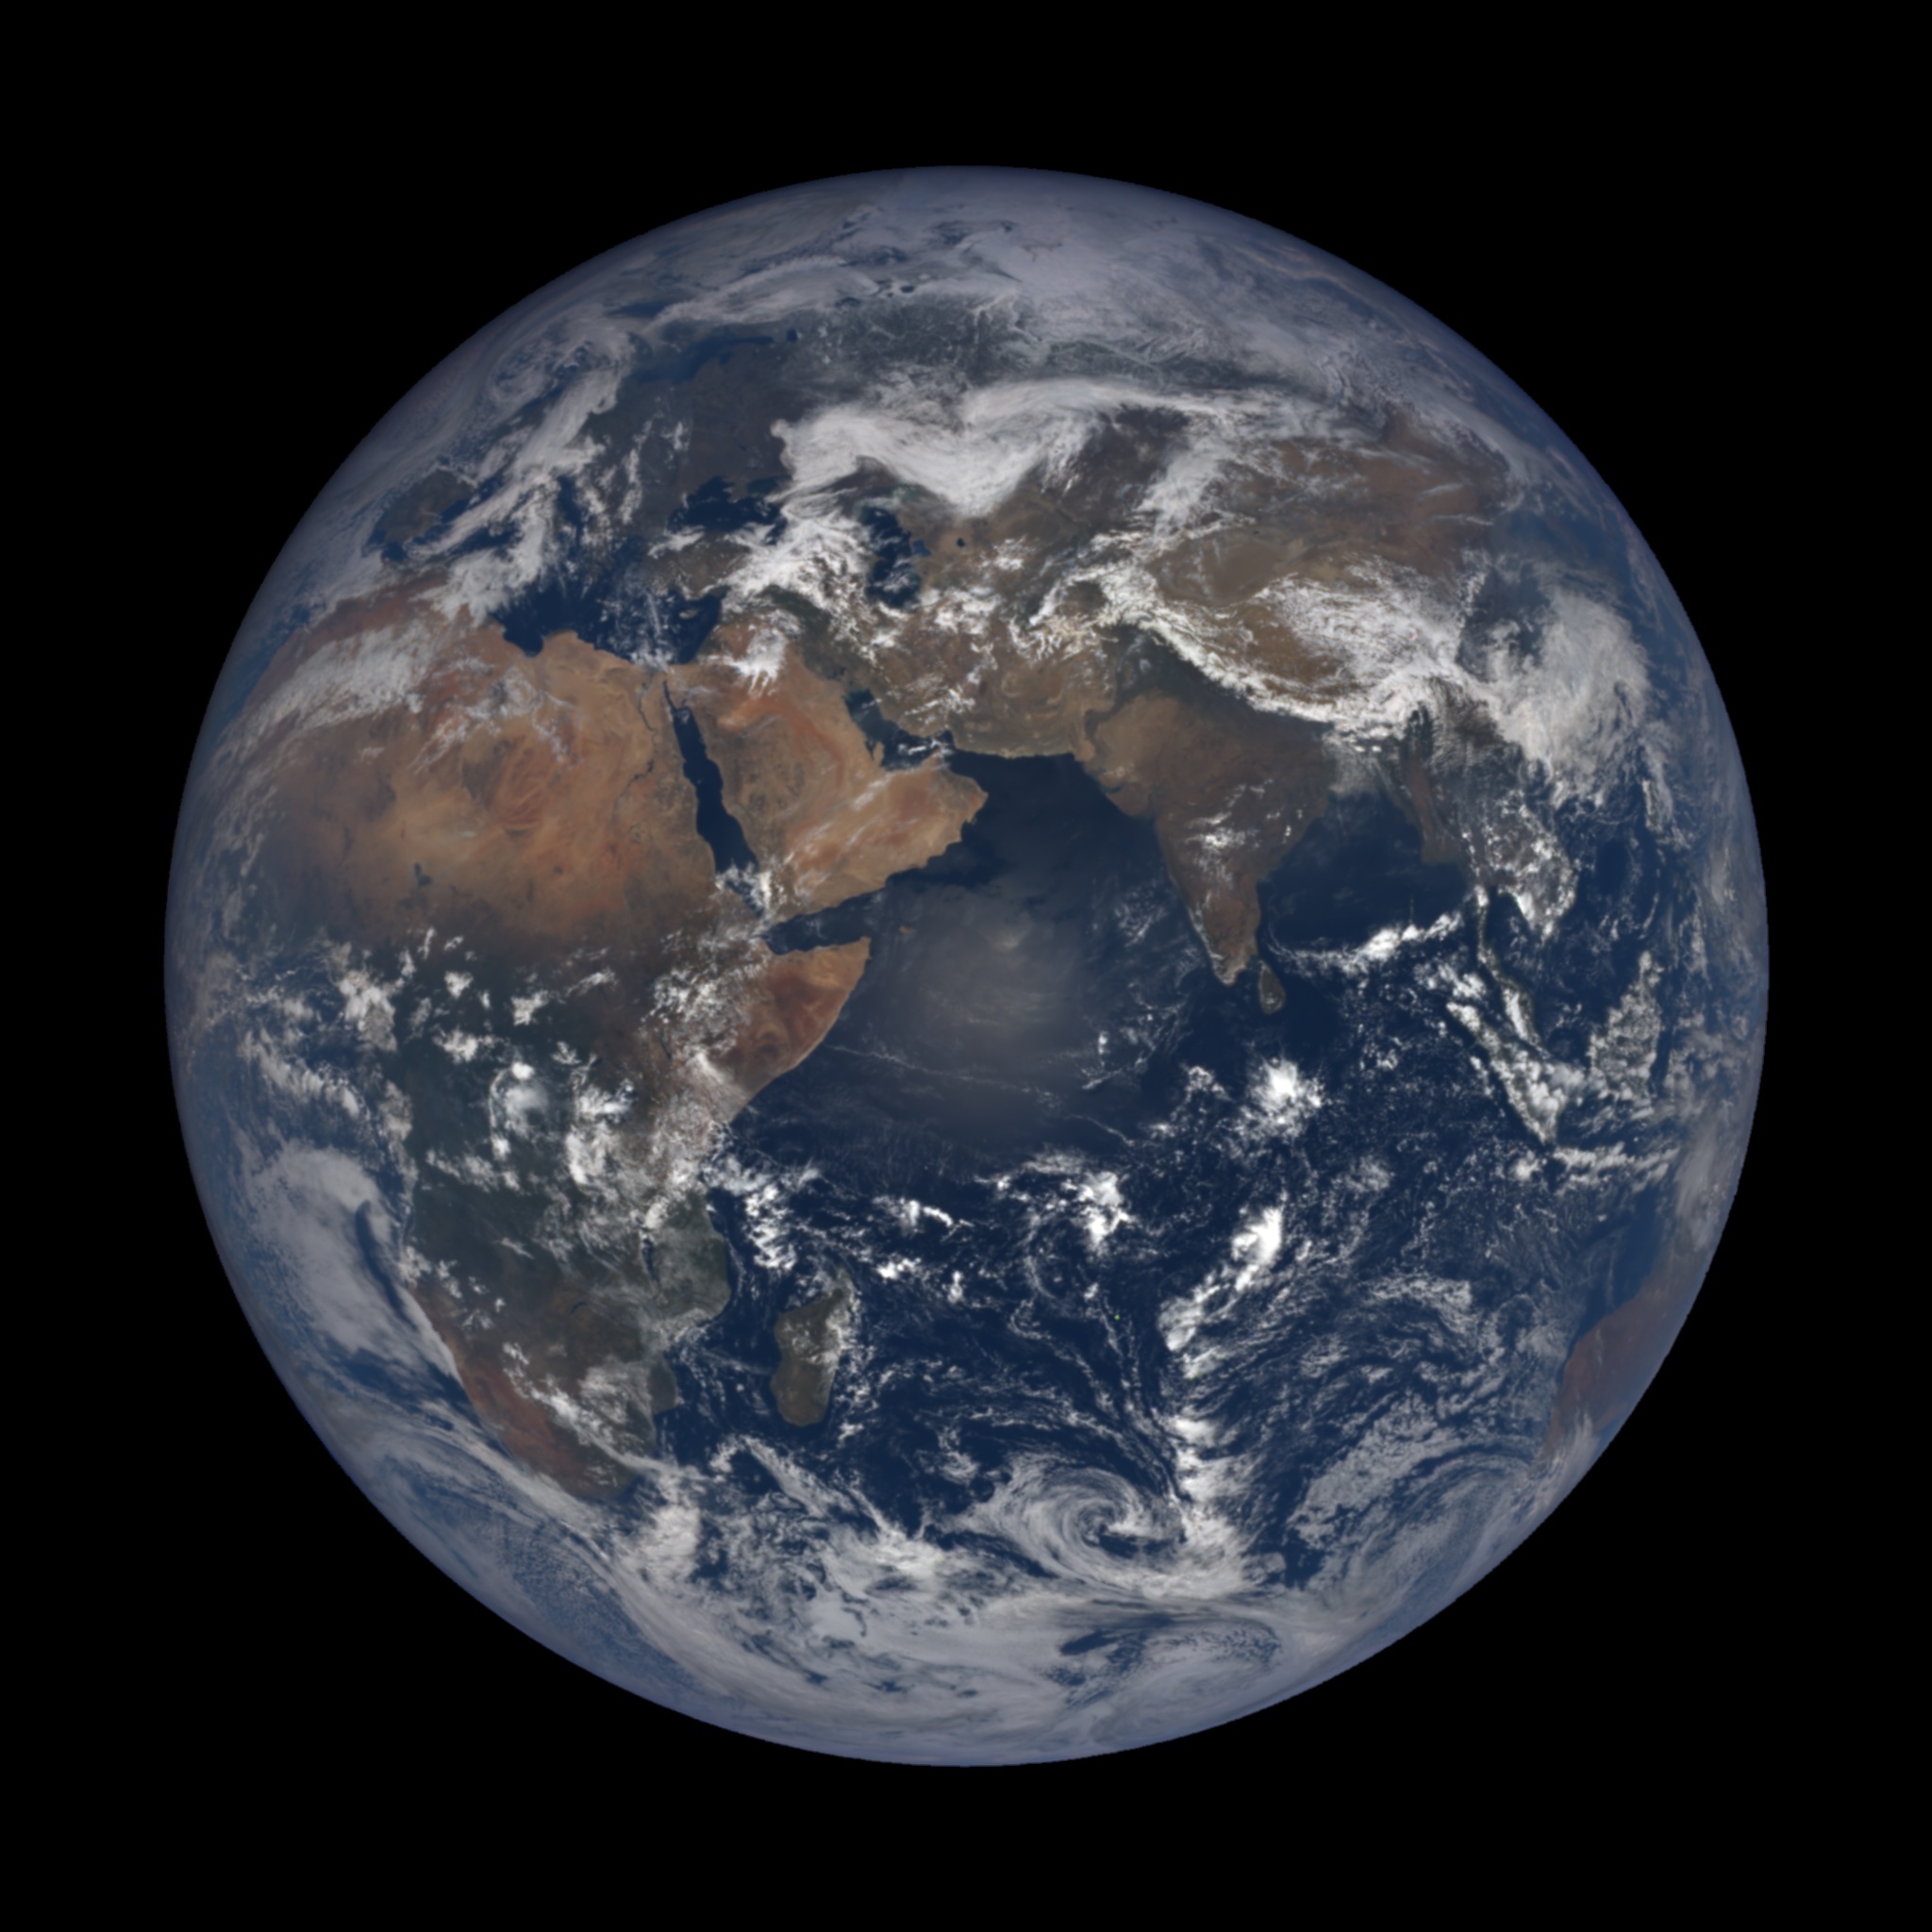
\includegraphics[width=5cm]{images/epic1}
			%\includegraphics[width=7cm]{images/fdl}
		\end{columns}
	\end{center}
	
	\vfill
\end{frame}
}

\begin{frame}
\frametitle{System Earth}

\begin{columns}
	
	\column{.5\textwidth}
	
	{
		%		The Earth is a complex system.
		%		Only some components is observable by 
		%		\begin{itemize}
		%			\item satellite-based or
		%			\item in-situ observations
		%		\end{itemize}
		%		
		
		%	\begin{equation*}\V{y} = f({\M{X}})\end{equation*}
		%	partially observe the complex system Earth
		\textbf{Partially measuring} System Earth
		{\Huge
			\begin{equation*}
			\M{X} = \sat\left({\earth}\right)
			\end{equation*}
		}
		
		\vspace{1em}
		\textbf{knowledge extraction} through pattern recognition and machine learning
		
		{\Huge\begin{equation*}\V{?} = f({\M{X}})\end{equation*}}
	}
	
	\column{.5\textwidth}
	
	\begin{tikzpicture}[xscale=3, yscale=2]
	\node(earth) at (0,0) {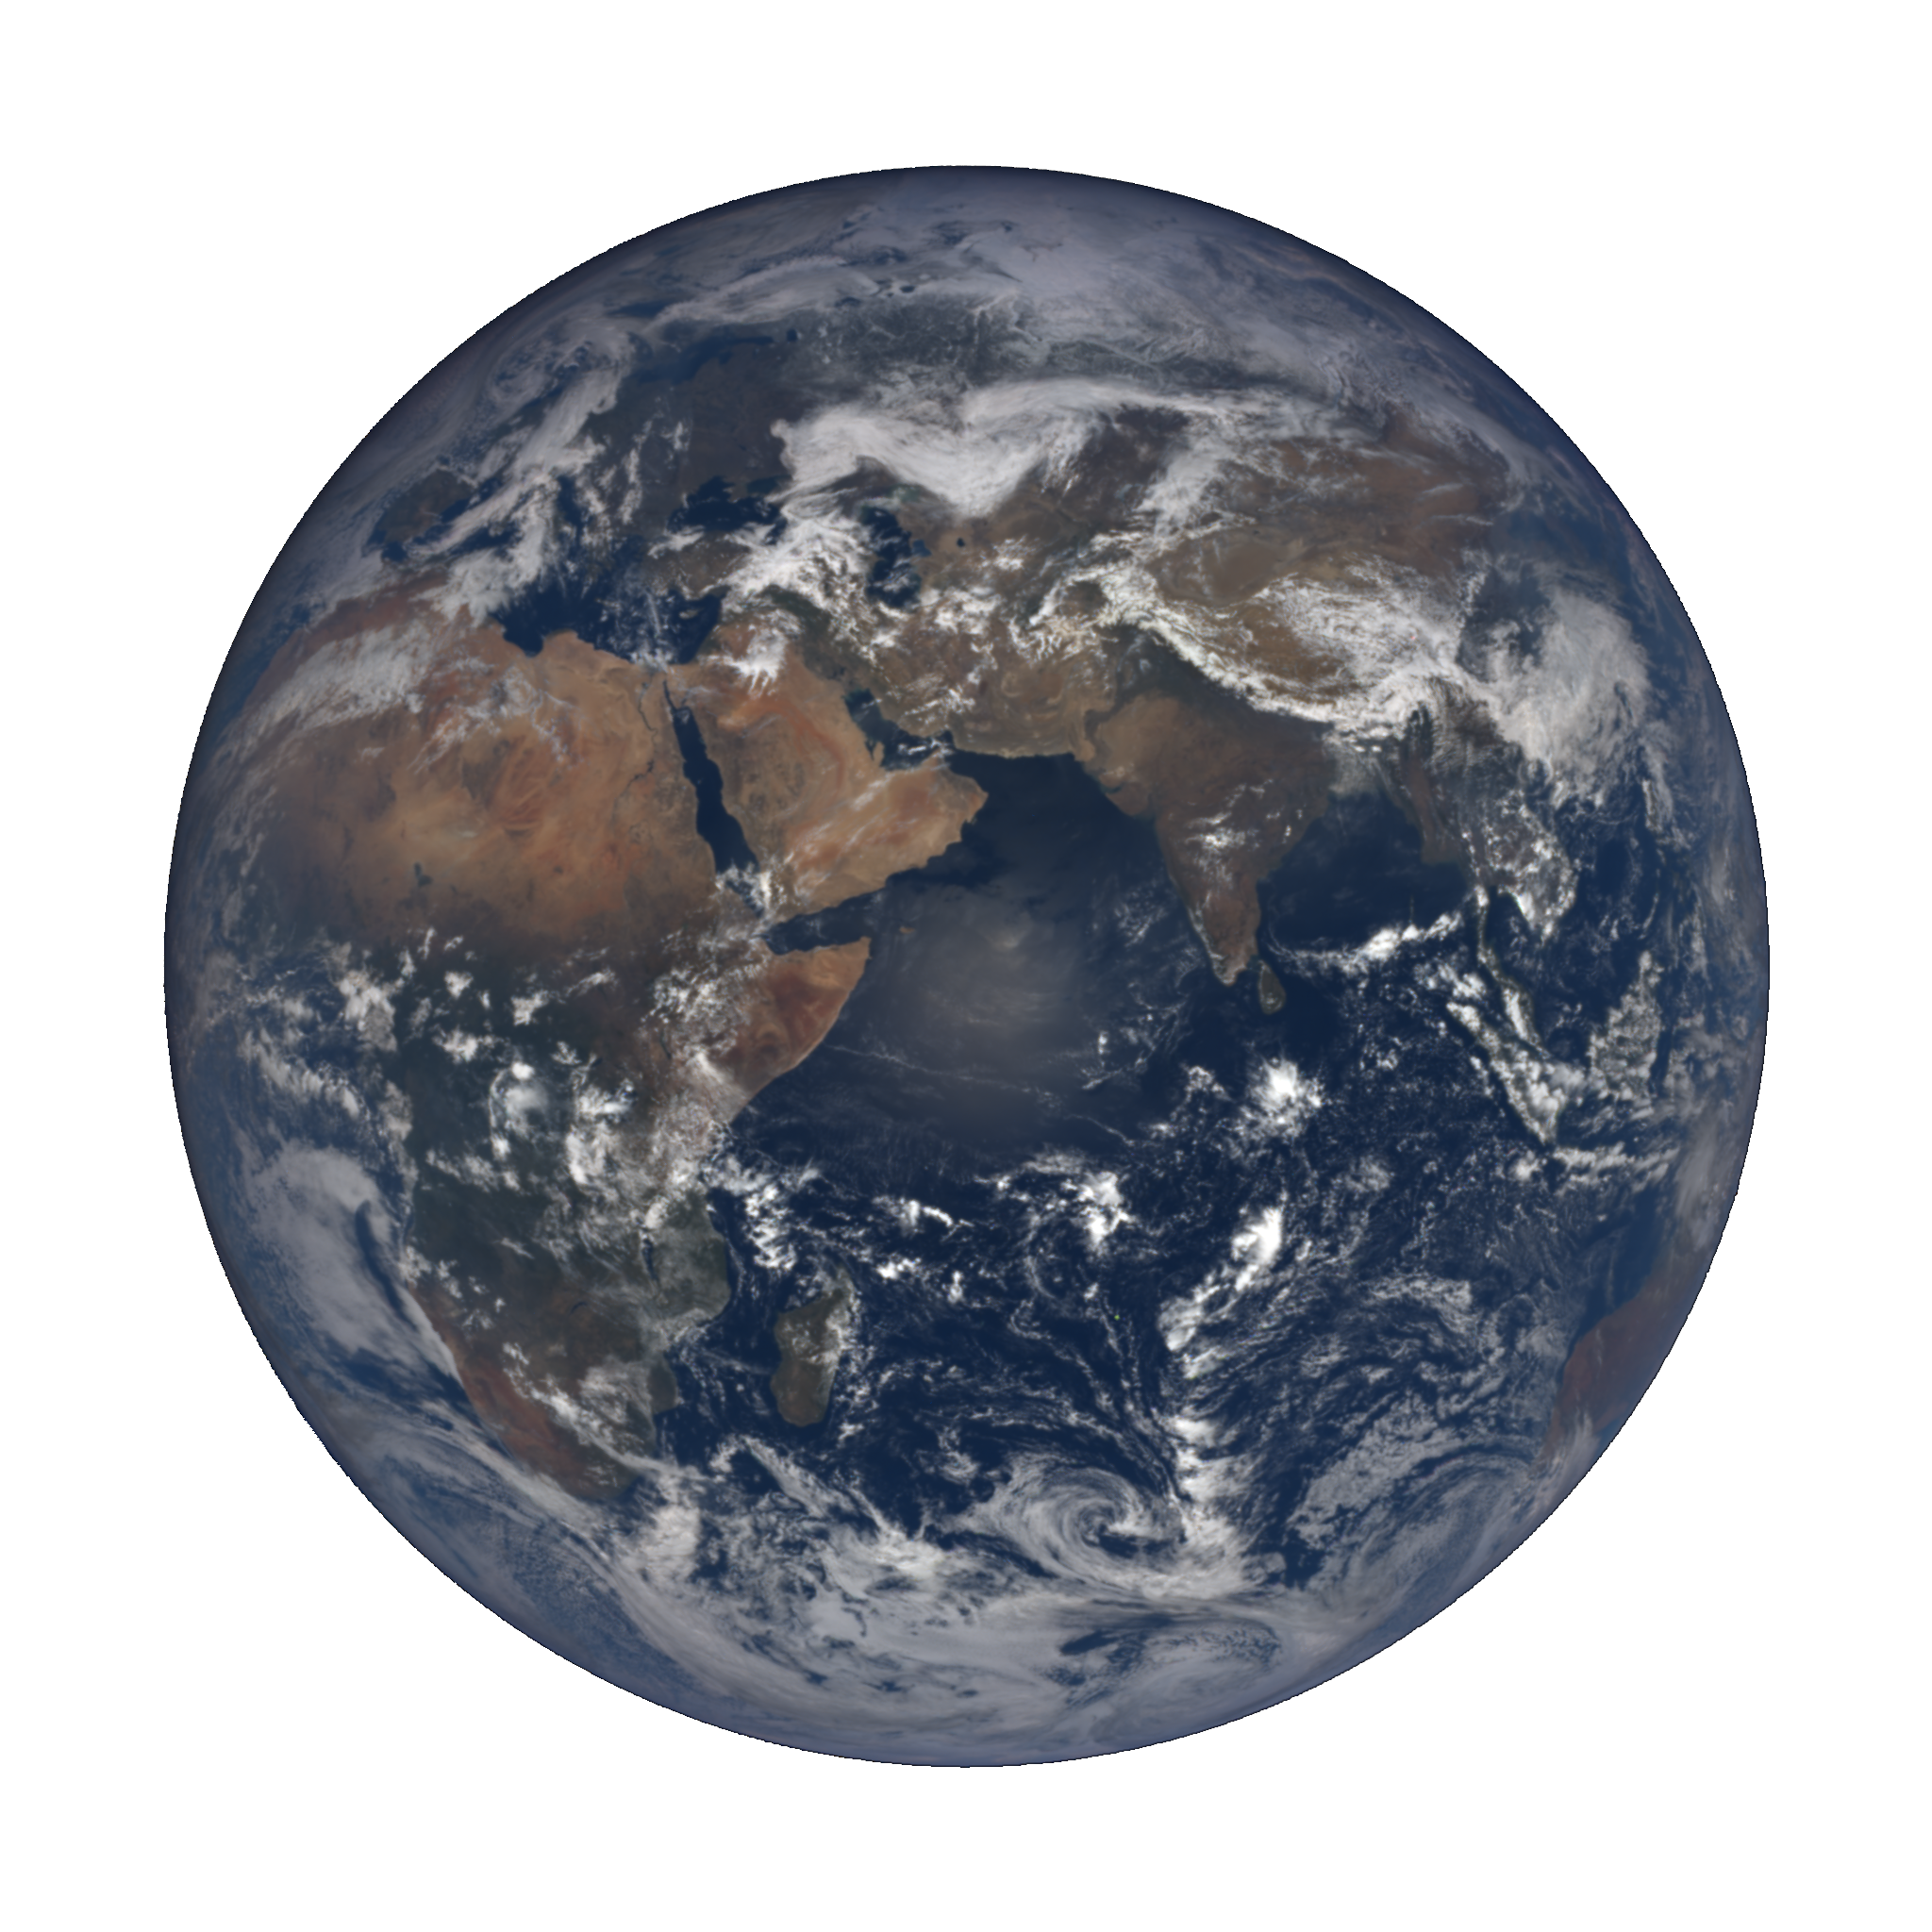
\includegraphics[width=7cm]{images/epicw1}};	
	
	\end{tikzpicture}
	
	
\end{columns}

%	\includegraphics[width=5cm]{images/Earth_gravity}
%	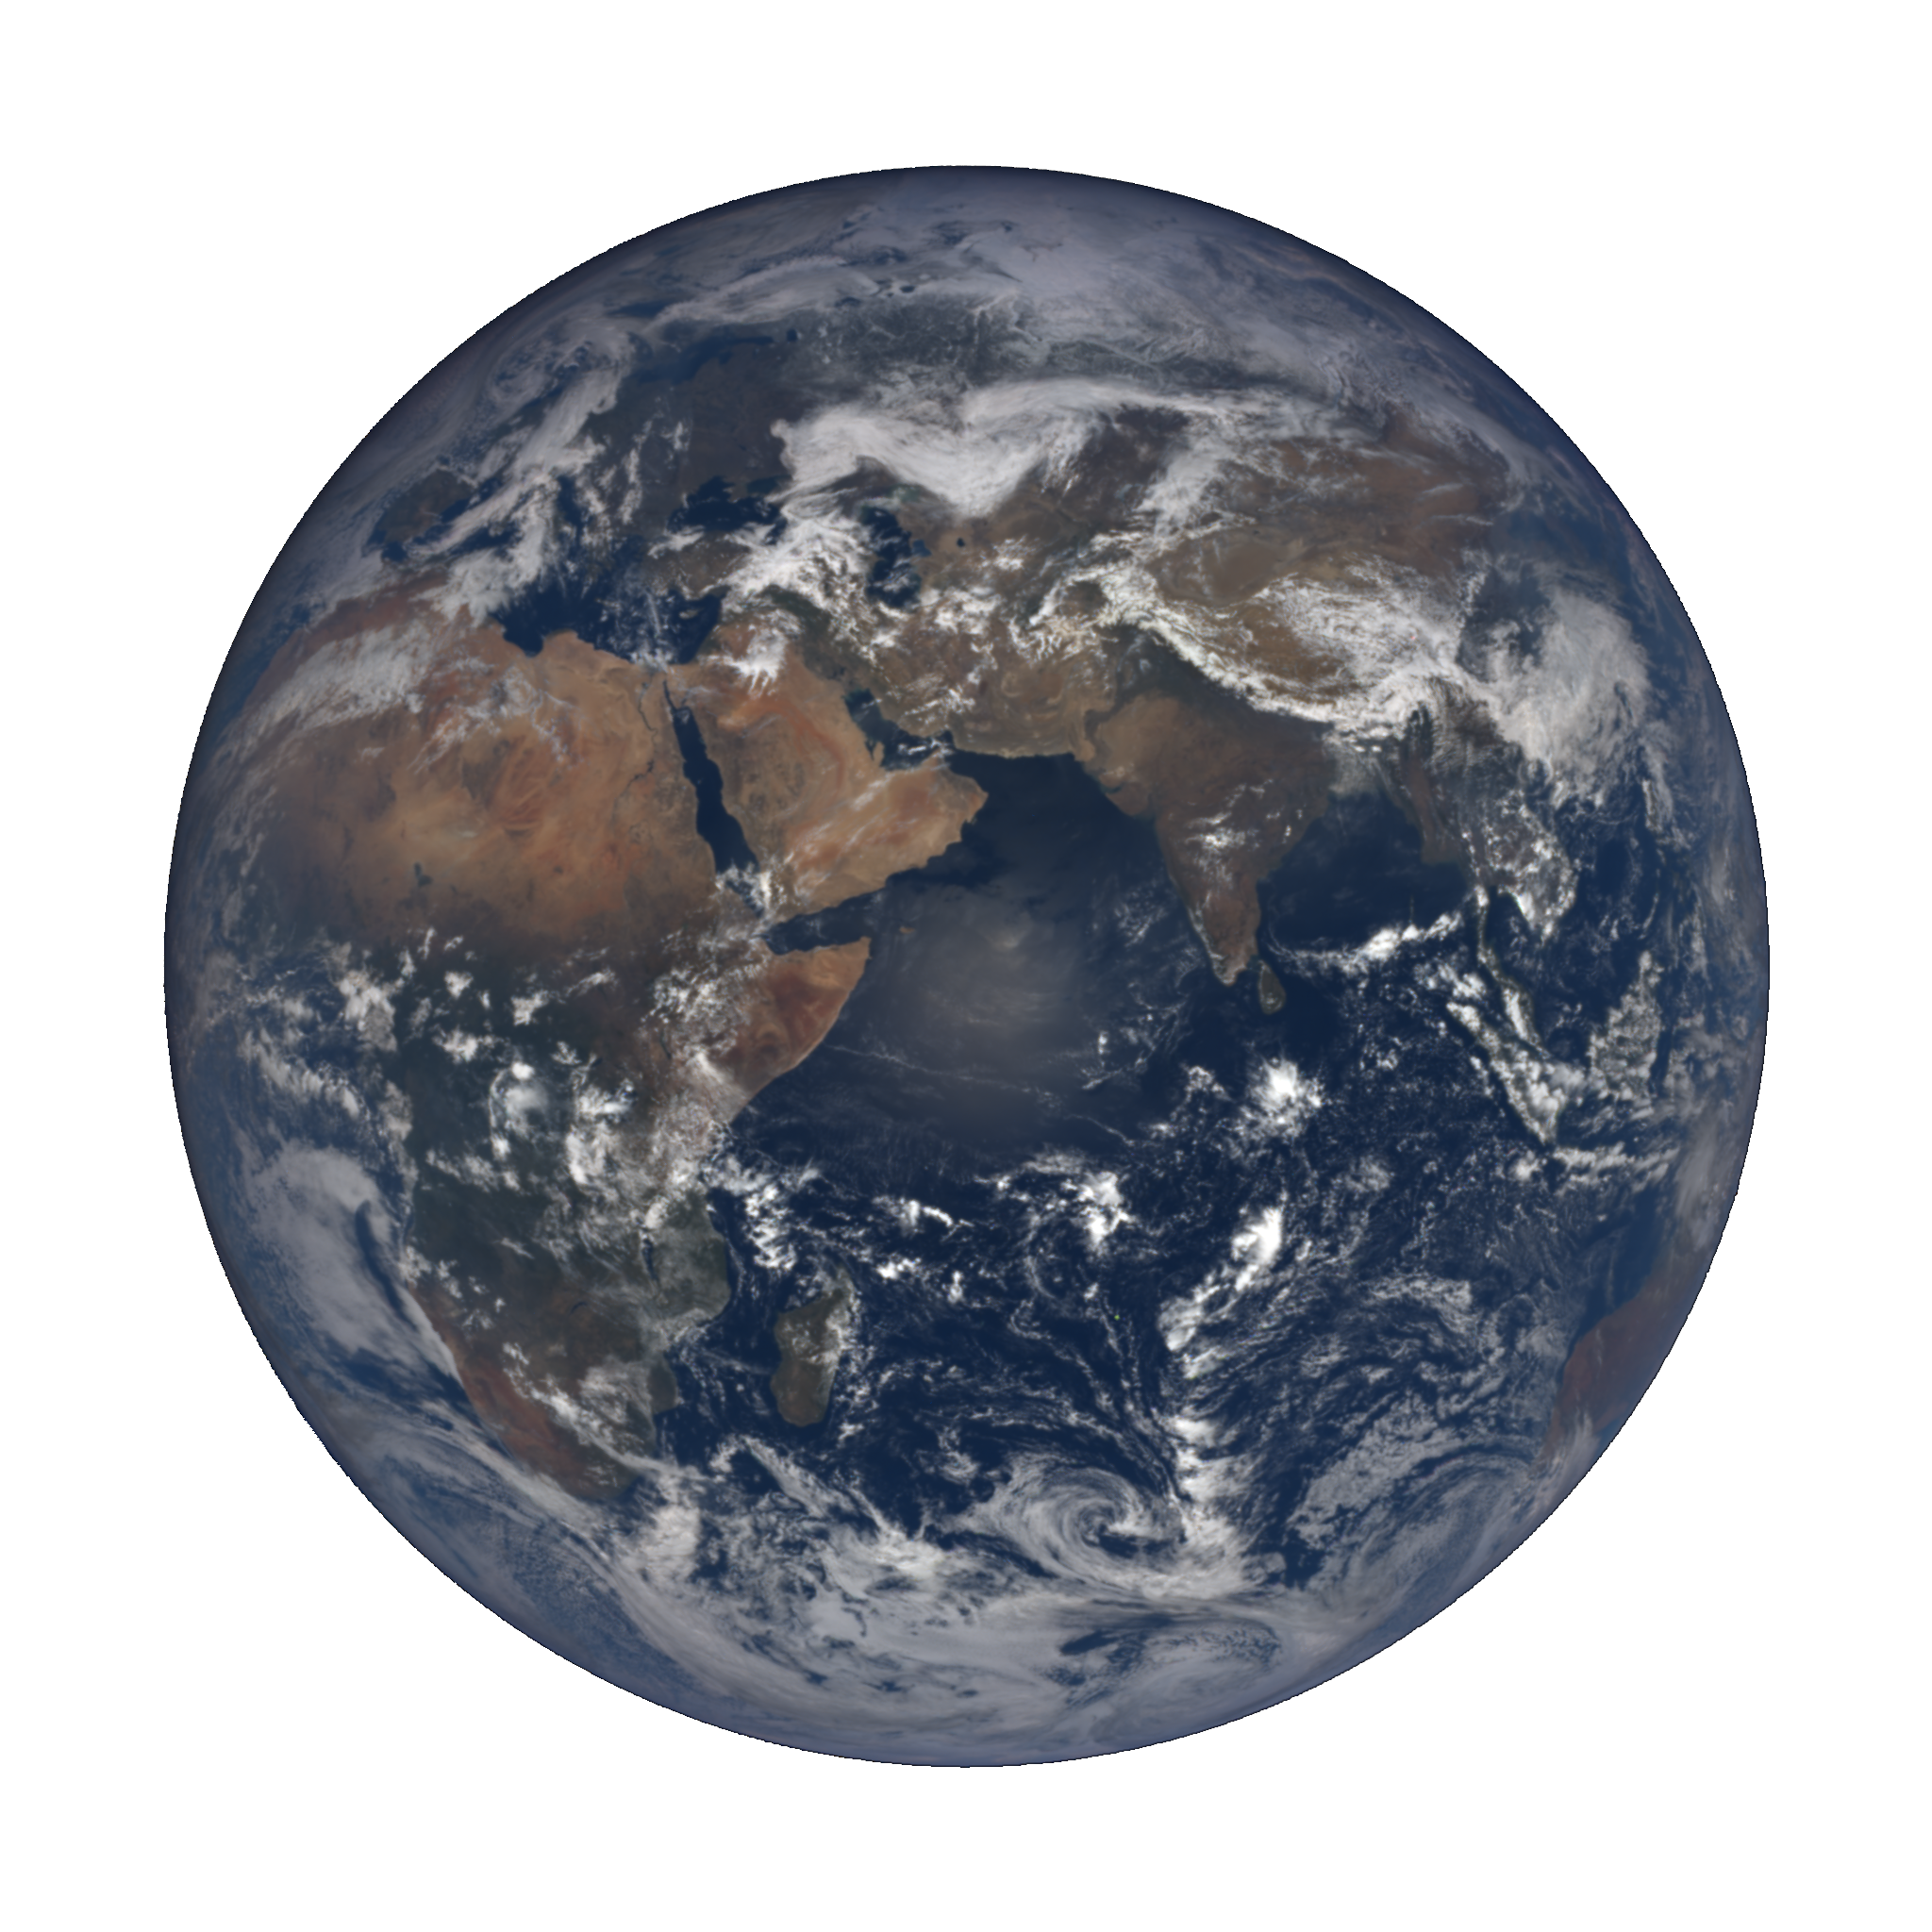
\includegraphics[width=5cm]{images/epicw1}
%	\includegraphics[width=5cm]{images/earthnullschool/sealevelpressure}
%	\includegraphics[width=5cm]{images/earthnullschool/misery_index}
%	\includegraphics[width=5cm]{images/earthnullschool/temp}
%	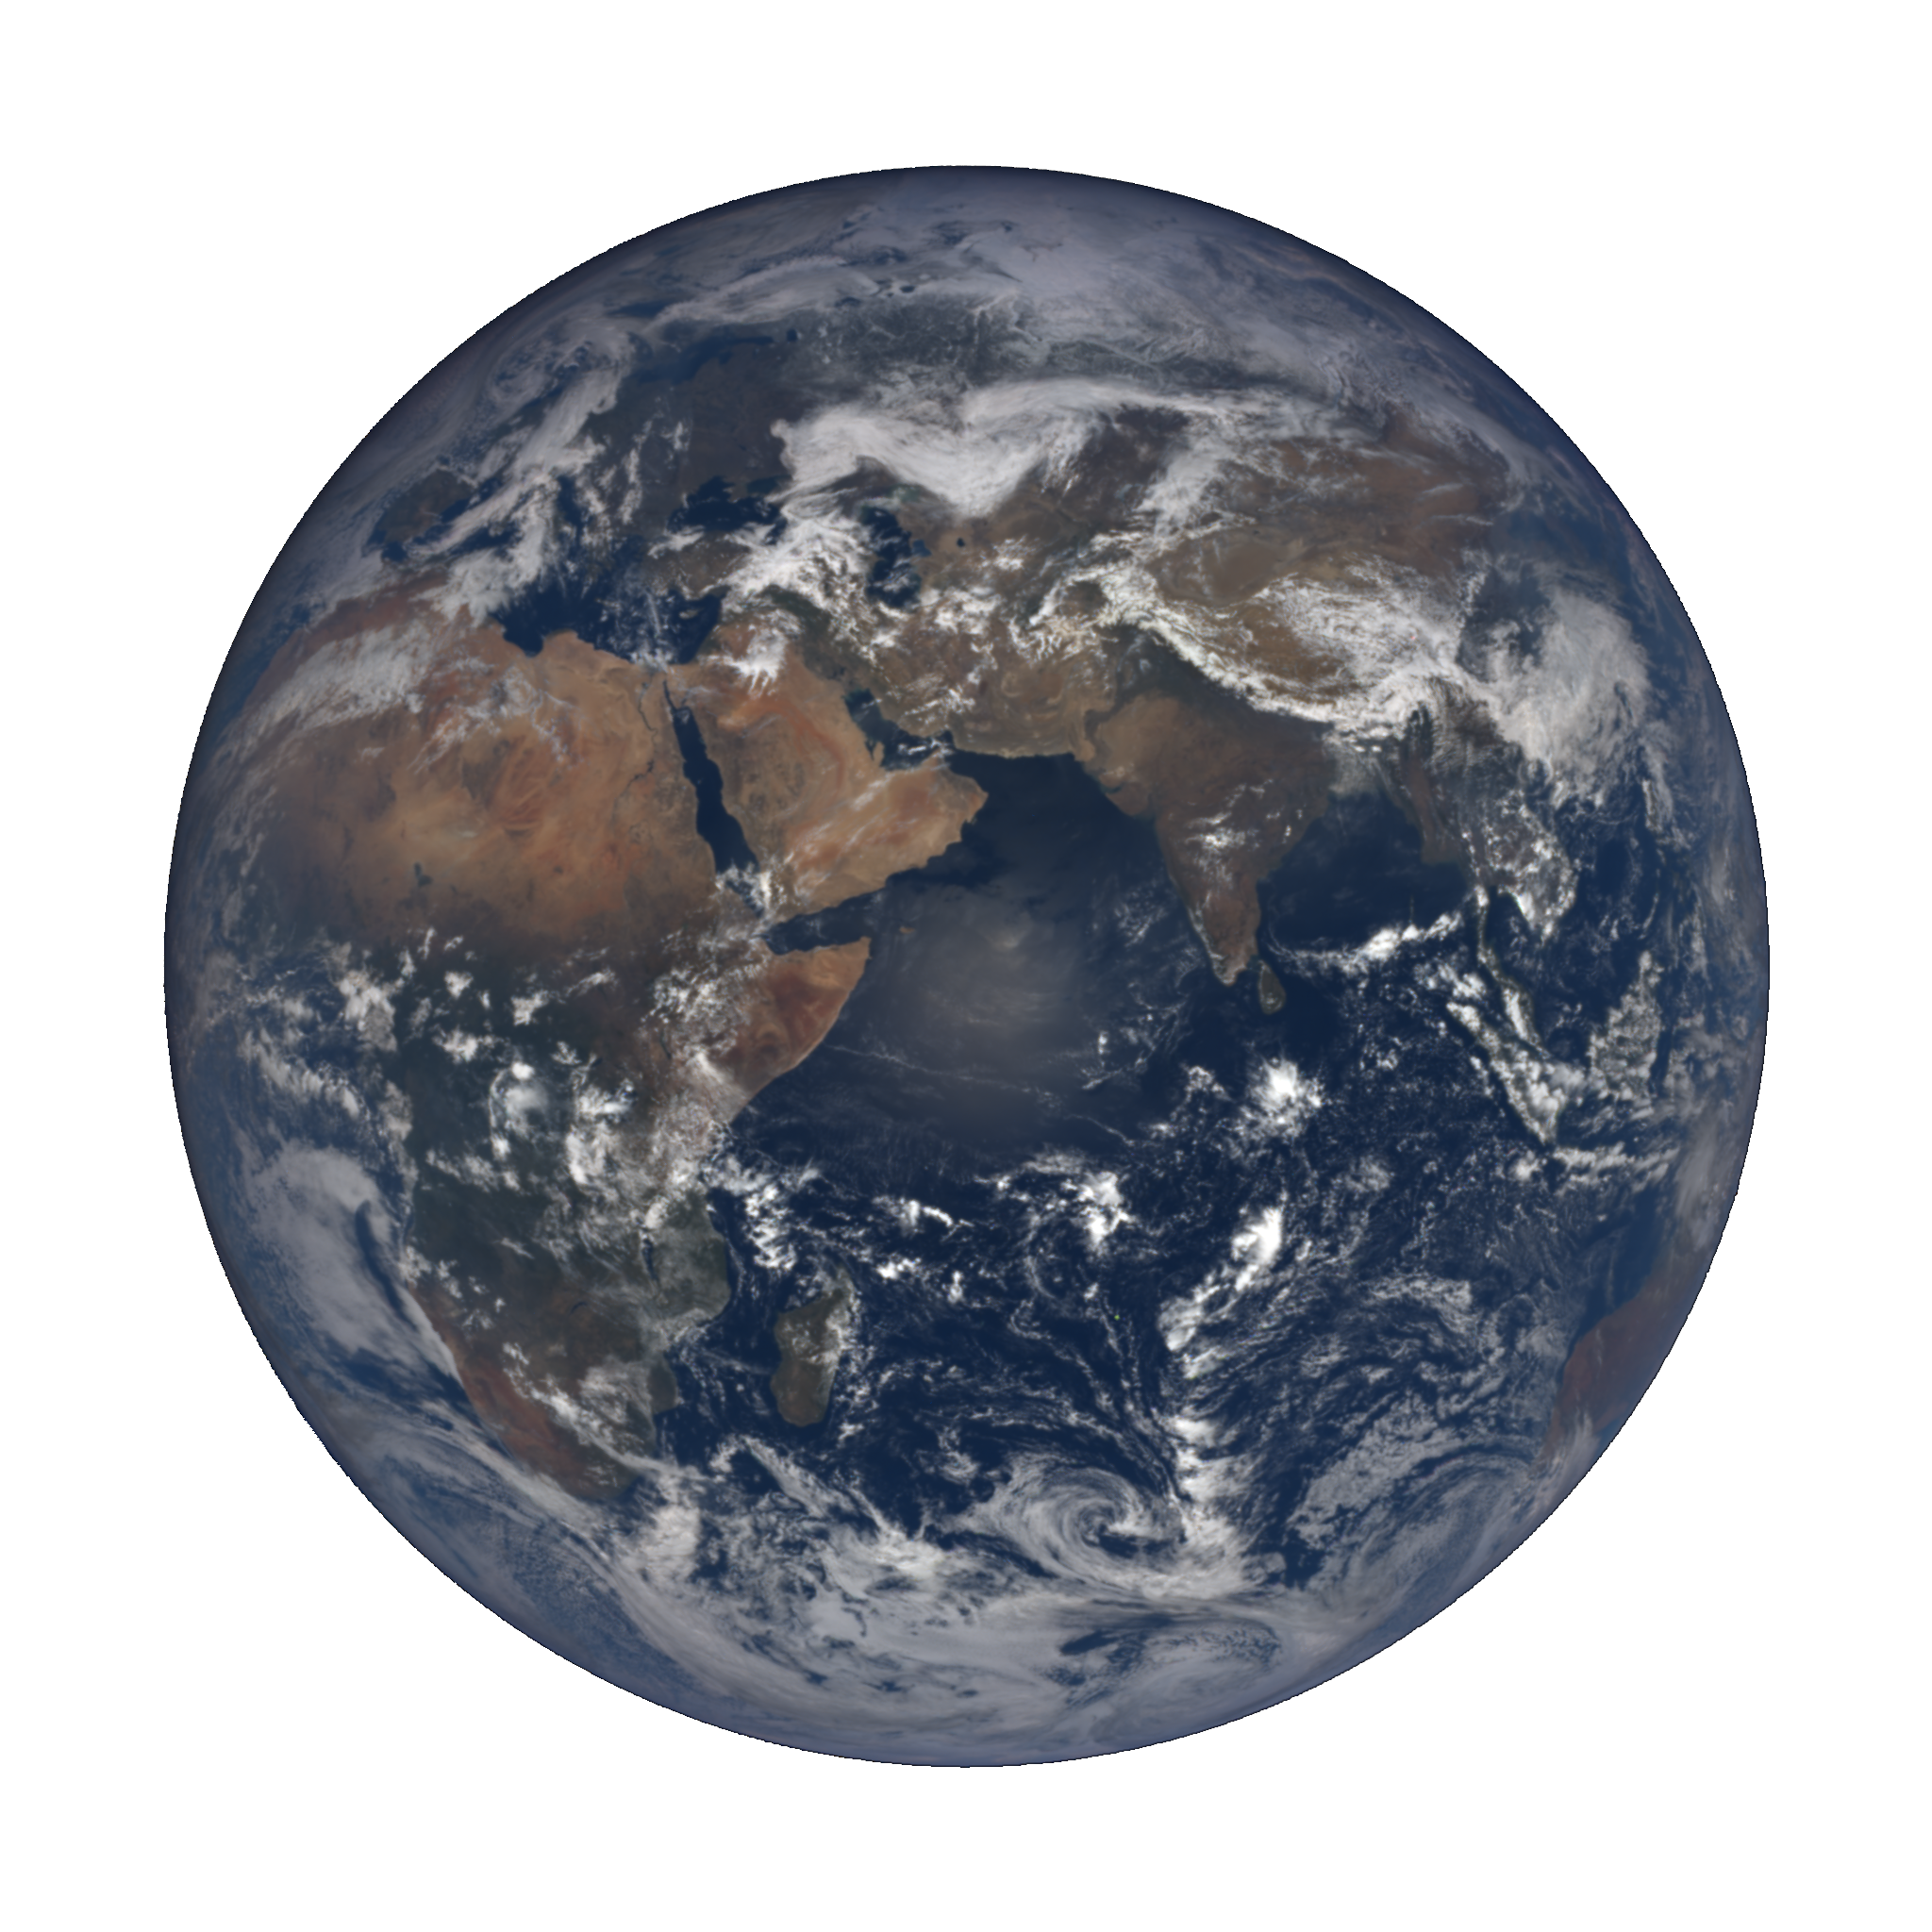
\includegraphics[width=5cm]{images/epicw1}
\end{frame}

%\begin{frame}
%\frametitle{Optical Satellites}
%\begin{columns}
%	\column{.5\textwidth}
%	
%%	
%%	\begin{itemize}[itemsep=.5em]
%%		\item<1-> Sensor measures \textbf{Digital Numbers} $\text{DN}(\lambda)$ for each wavelength $\lambda$. 
%%		\item<2-> \textbf{Digital Numbers} are normalized to \textbf{Radiance} 
%%		$L(\lambda), \left[\frac{W}{\text{sr}m^2}\right]$ by gain and offset calibration.
%%		\item<3-> Radiance is normalized to \textbf{top-of-atmosphere reflectance} $\rho(\lambda)$
%%		%		\item<4-> \textbf{Bottom-of-atmosphere reflectances} are reconstructed using a functional model of the atmosphere.
%%	\end{itemize}
%%	
%	%	Radiance $R_\lambda$ from measured Digital Numbers via calibrated gain $\alpha$ and offset $\beta$
%	%	\begin{equation*}
%	%		L_\lambda = \alpha \text{DN}_\lambda + \beta, \left[\frac{W}{\text{sr}m^1}\right]
%	%	\end{equation*}
%	%	
%	%	top-of-atmosphere reflectance $\rho_\lambda$ as normalized Radiance $R_\lambda$ with solar 
%	%	\begin{equation*}
%	%	\rho_\lambda = \frac{L_\lambda}{\cos(\varphi_\text{sun})}
%	%	\frac{
%	%		\pi d^2
%	%	}
%	%	{
%	%		E_\text{sun}(\lambda)
%	%	}
%	%	\end{equation*}
%	%	
%	%	\vspace{1em}
%	%	
%	%	\begin{itemize}
%	%		\item measured radiance $L(\lambda)$
%	%		\item solar irradiance $E_\text{sun}(\lambda)$
%	%		\item solar zenith angle $\varphi_\text{sun}$
%	%		\item squared Earth-Sun distance $d$ in AU
%	%	\end{itemize}
%	
%	
%	\column{.5\textwidth}
%	
%	
%	\begin{tikzpicture}
%	
%	
%	%	\draw [black,dotted, fill=tumbluelight,domain=110:70] plot ({13*cos(\x)}, {13*sin(\x)-12.8});
%	\draw [fill=tumivory,domain=110:70] plot ({10*cos(\x)}, {10*sin(\x)-10});
%	%	\draw [fill=tumbluelight,domain=110:70] plot ({12*cos(\x)}f, {12*sin(\x)-10});
%	
%	
%	\node(sun) at (-2,2) {
\includegraphics[width=10mm]{images/icons/sun}};
%	\node[rotate=130,anchor=center](sat) at (2,2) {
\includegraphics[width=10mm]{images/icons/sat2}};
%	
%	\node(px) at ({10*cos(90)}, {10*sin(90)-10.1}){
%		\begin{tikzpicture}[xscale=.5,yscale=.25]
%		\draw[fill=tumbluelight] (0,0) -- (1,0) -- (2,1) -- (1,1) -- (0,0);
%		\end{tikzpicture}
%		%
\includegraphics[width=5mm]{images/icons/house}
%	};
%	
%	\draw[-stealth] (sun) -- node[midway,sloped]{\wave} (px);
%	\draw[-stealth] (px) -- node[midway,sloped]{\wave} (sat);
%	
%	\visible<3->{\draw[-stealth] (sun) -- node[midway,sloped]{\wave} (sat);
%		\draw[draw=tumgray] (px) -- node[at end,left]{$\varphi_\text{sun}$} ++(0,1.4); 
%		\draw [draw=tumgray, domain=130:90] plot ({1*cos(\x)}, {1*sin(\x)});
%	}
%	
%	\node[above=.5em of sun]{$E_\text{sun}(\lambda)$};
%	\visible<1>{\node[above=4em of sat]{$DN(\lambda)$};}
%	\visible<2>{\node[above=4em of sat]{$L(\lambda)$};}
%	\visible<3>{\node[above=4em of sat]{$\rho_\text{toa}(\lambda)$};}
%	%	\visible<4>{\node[above=4em of sat]{$\rho_\text{boa}(\lambda)$};}
%	
%	%		\draw[red] (0,0) sin (1,2);
%	
%\end{tikzpicture}
%\end{columns}
%\end{frame}

\begin{frame}
\frametitle{Acquired in regular time intervals}
\framesubtitle{Sentinel 2 Satellite}

%	\includemovie[
%	poster,
%	text={\small(Loading Circle-m-increase3.mp4)}
%	]{6cm}{6cm}{images/s2orbits.mp4}
%	
%	\movie{loaded}{images/s2orbits.avi}

\begin{columns}
\column{.5\textwidth}

\Large
\begin{itemize}
\item<1-> polar sun-synchronous orbit
\item<2-> single orbit circa 100 minutes
\item<3-> revisit same location after 5 days
\item<4-> acquisition stripe of 290km width
\item<5-> 13 spectral bands
\item<6-> ground resolution 10-60m
\item<7-> global coverage and free of charge
\end{itemize}

\column{.5\textwidth}
%		\only<1>{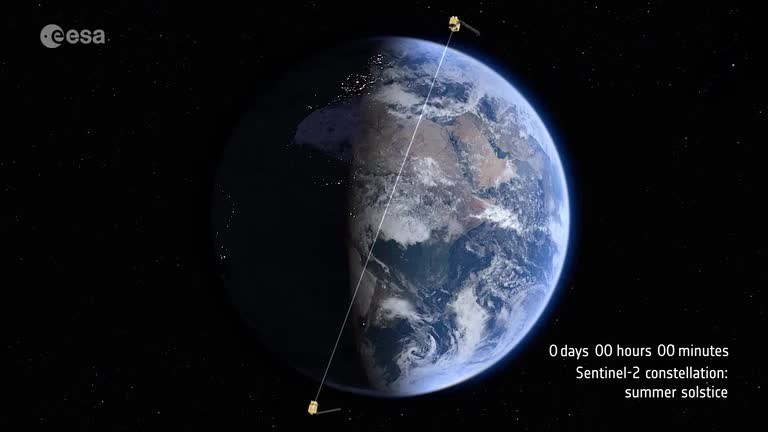
\includegraphics[width=\textwidth]{images/s2orbits/1}}
%		\only<2>{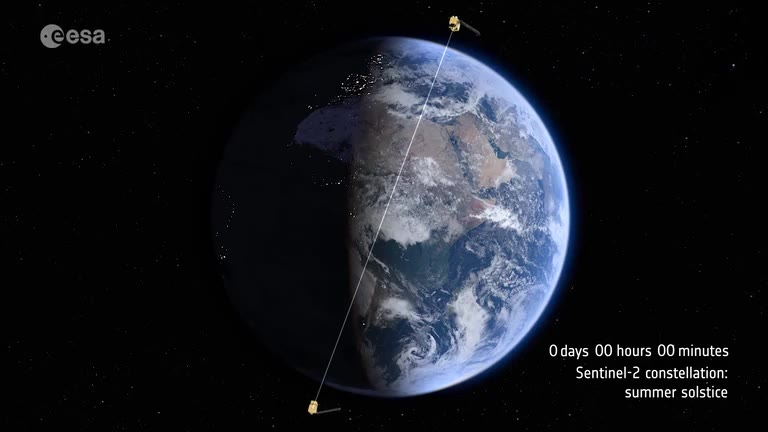
\includegraphics[width=\textwidth]{images/s2orbits/2}}
%		\only<3>{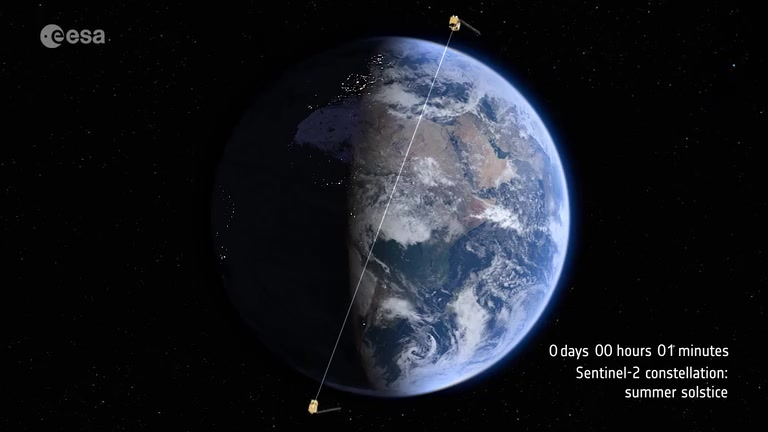
\includegraphics[width=\textwidth]{images/s2orbits/3}}
\only<1>{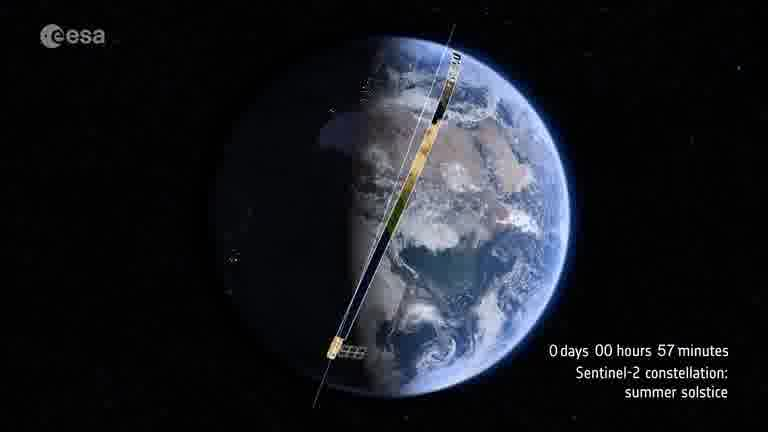
\includegraphics[width=\textwidth]{images/s2orbits/14}}
\only<2>{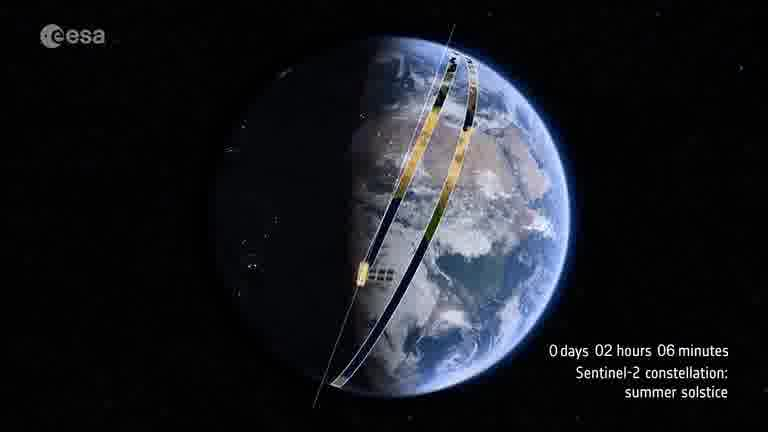
\includegraphics[width=\textwidth]{images/s2orbits/19}}
\only<3>{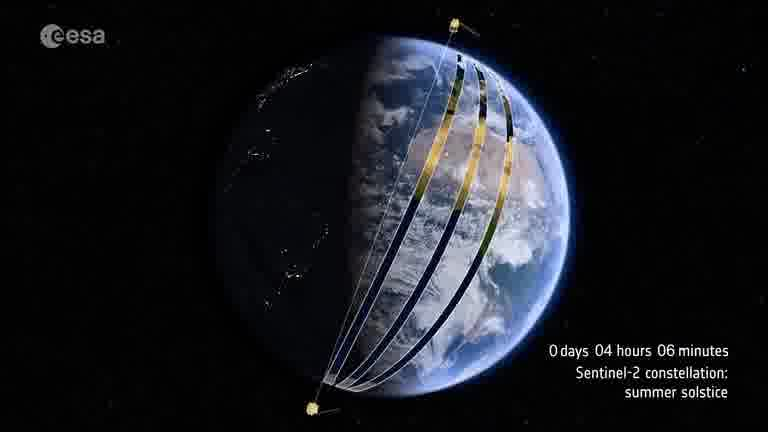
\includegraphics[width=\textwidth]{images/s2orbits/24}}
\only<4>{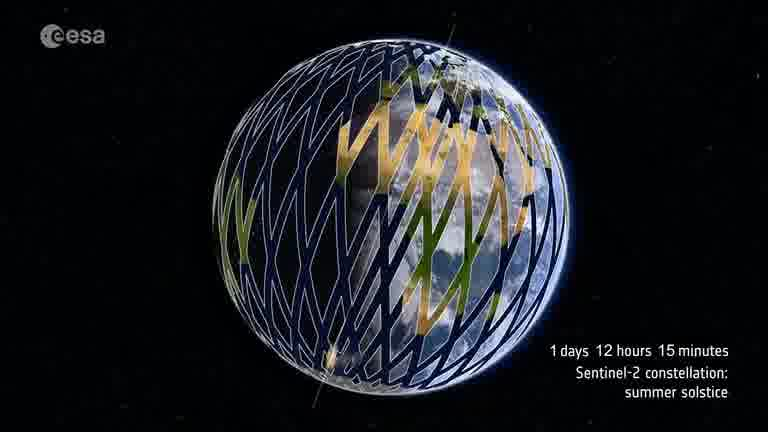
\includegraphics[width=\textwidth]{images/s2orbits/35}}
\only<5>{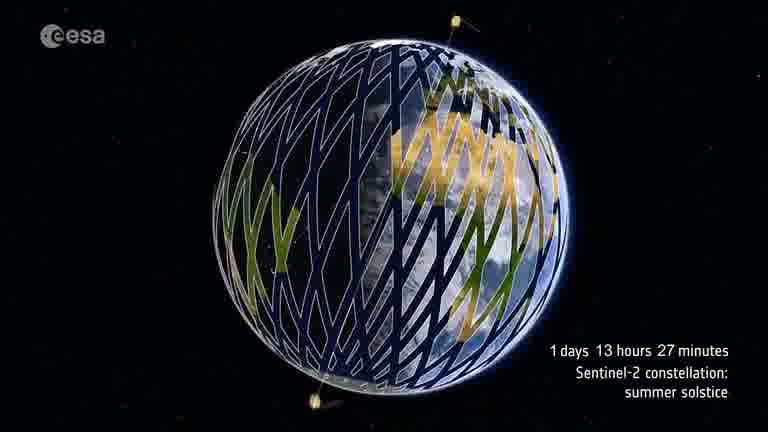
\includegraphics[width=\textwidth]{images/s2orbits/36}}
\only<6>{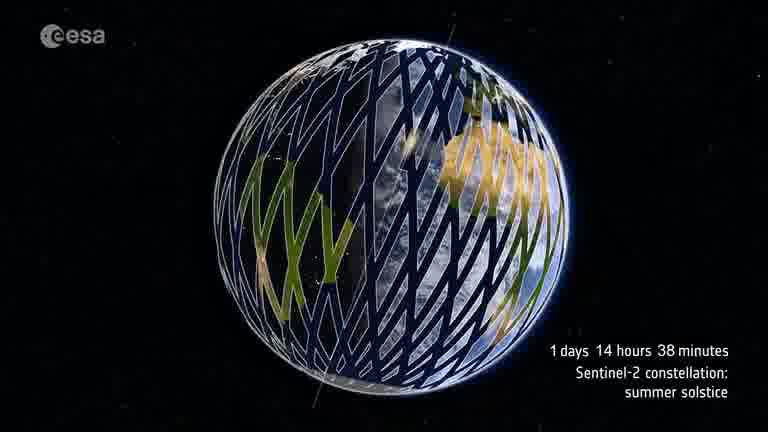
\includegraphics[width=\textwidth]{images/s2orbits/37}}
\only<7>{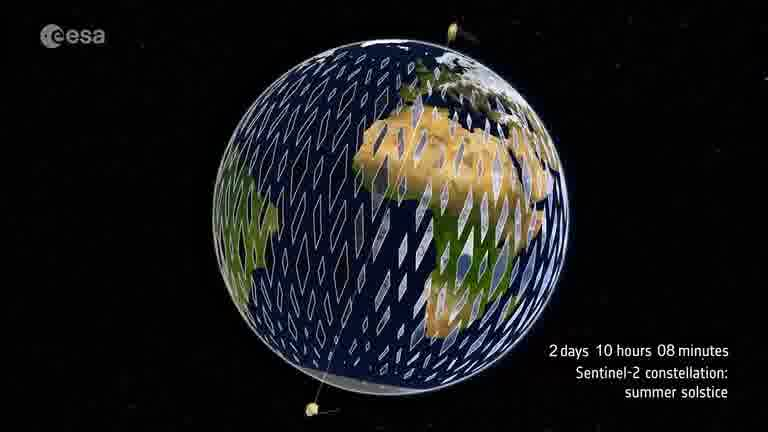
\includegraphics[width=\textwidth]{images/s2orbits/48}}
\tiny\url{https://www.esa.int/spaceinvideos/Videos/2016/08/Sentinel-2_global_coverage}
\end{columns}

\end{frame}

%
%
%{\setbeamercolor{background canvas}{bg=tumblack}
%	\begin{frame}[plain]
%	
%	\vfill
%	\Huge\color{white}
%	\begin{center}
%		\begin{columns}
%			\column{.5\textwidth}
%			\vspace{7em}
%			
%			\hfill 
%			Satellite Data Take-away
%			\column{.5\textwidth}
%			
%			
%			%%			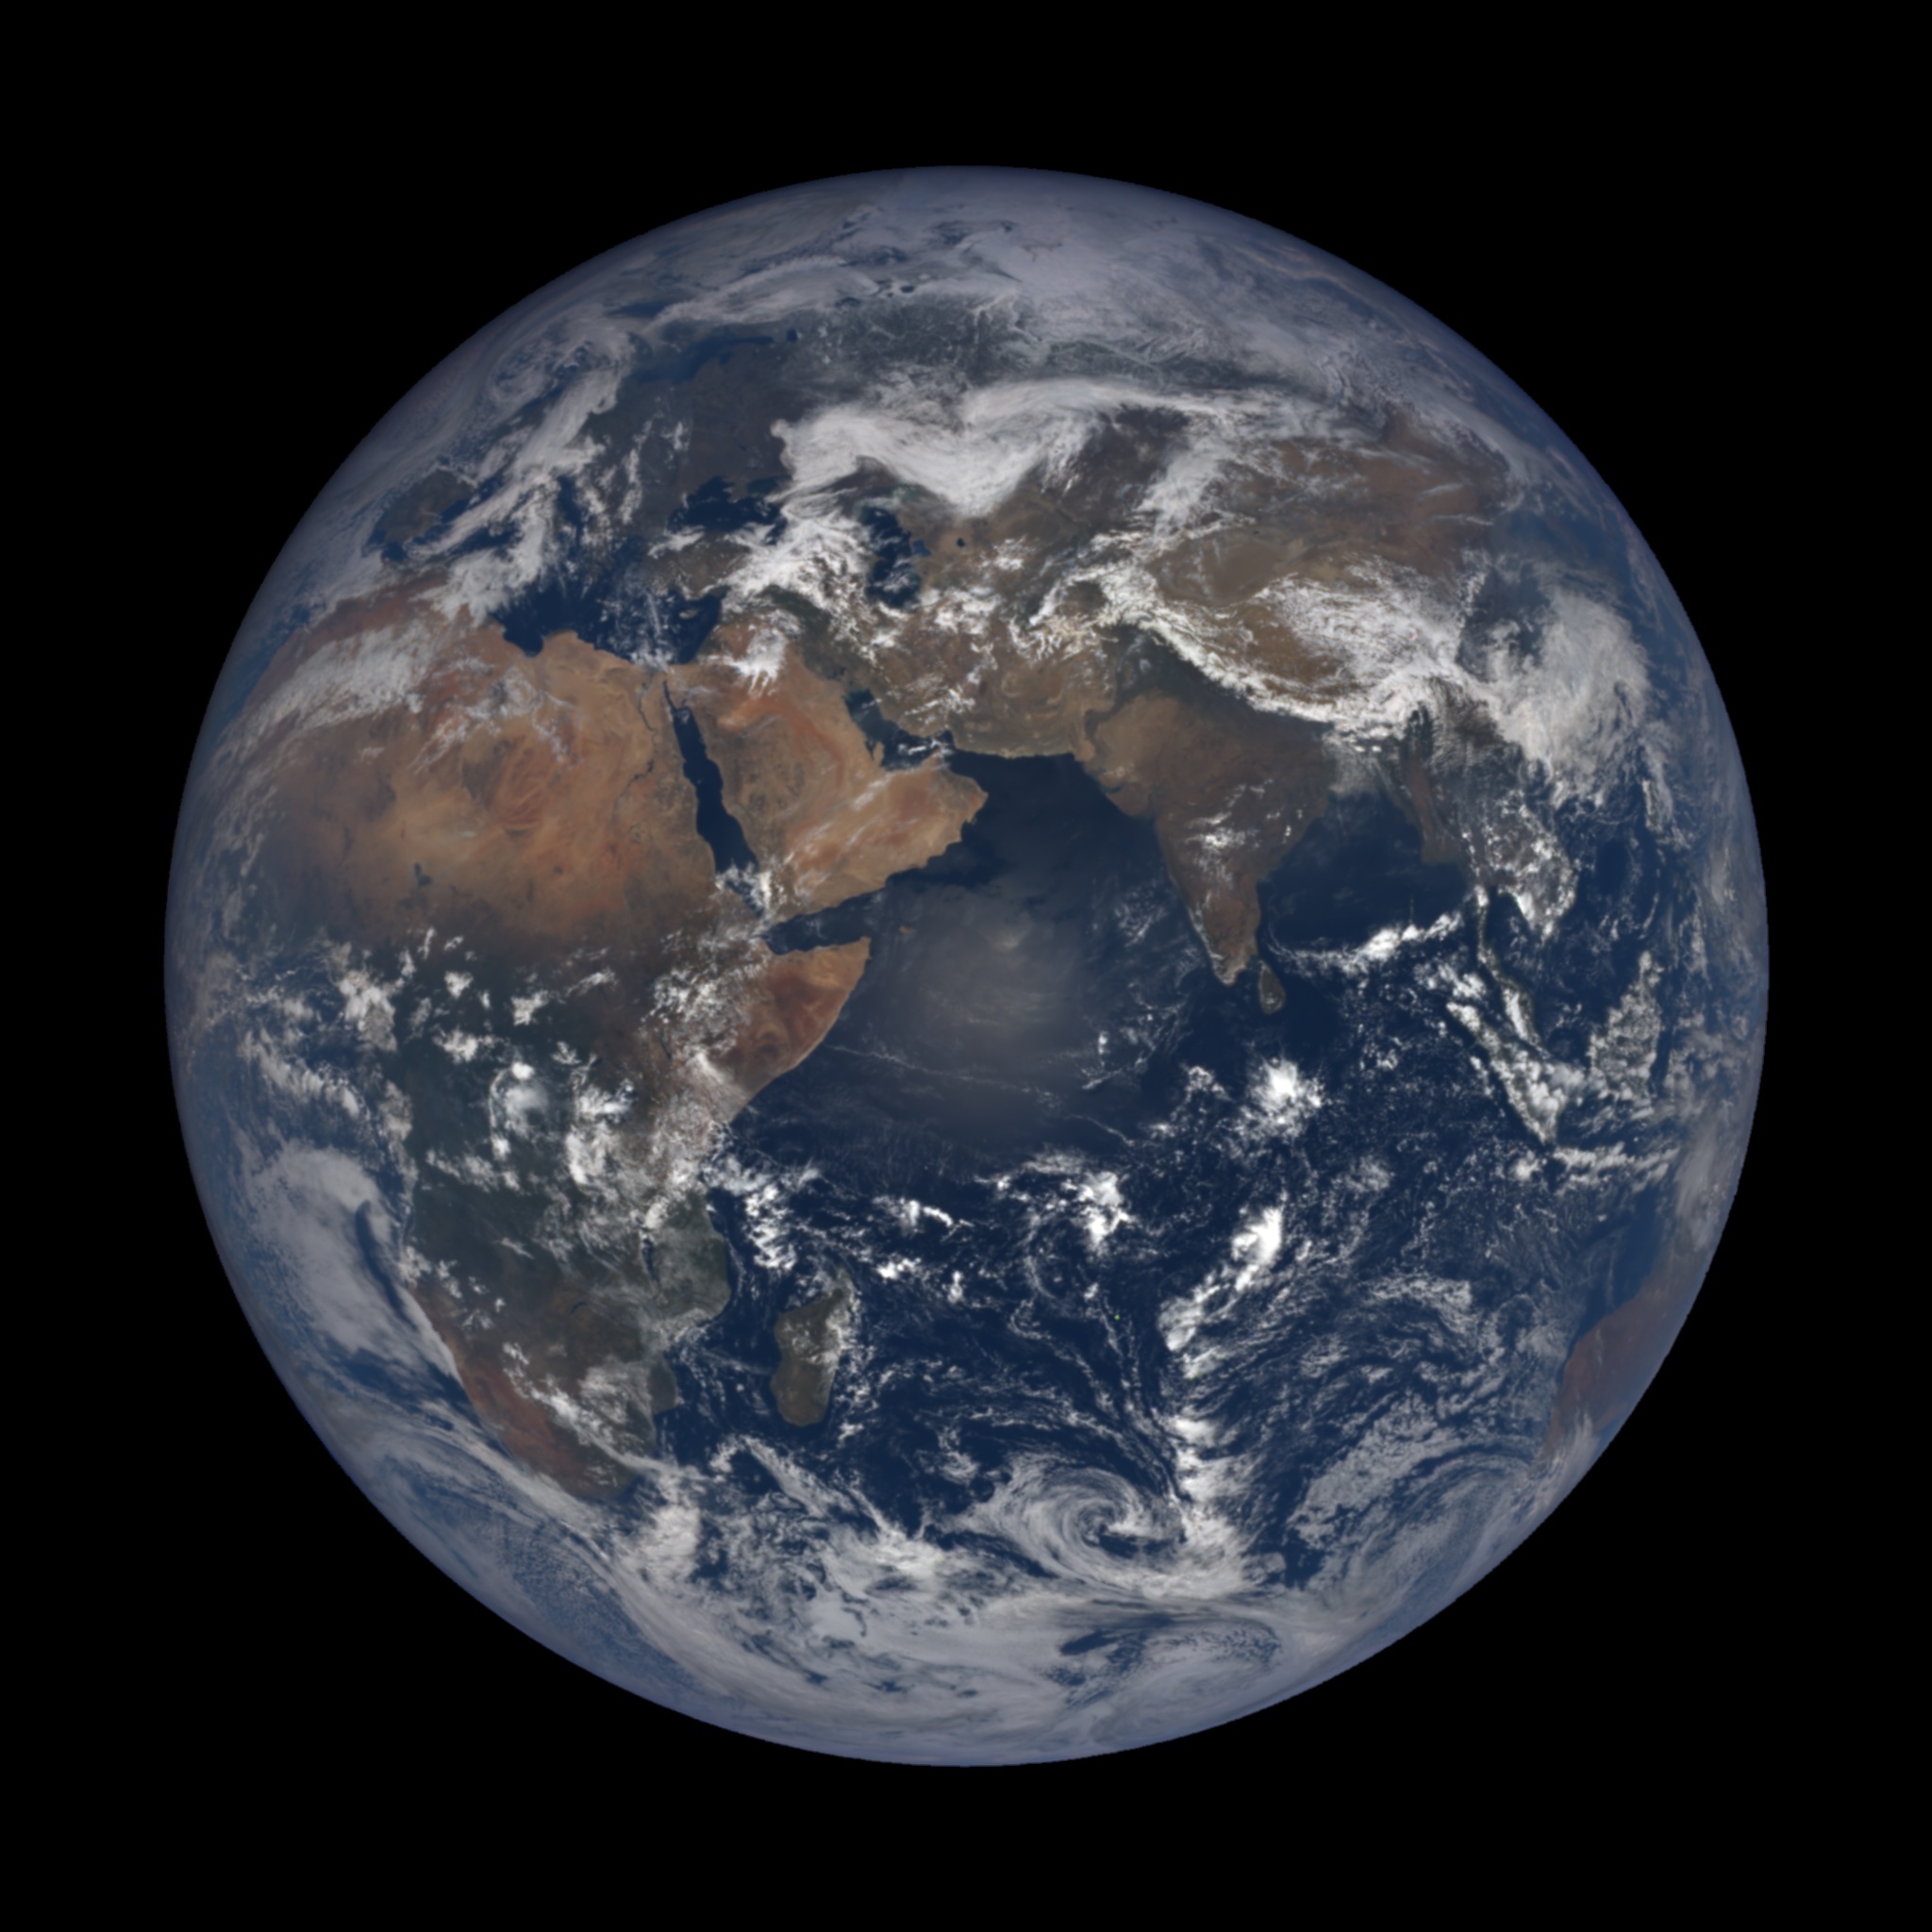
\includegraphics[width=5cm]{images/epic1}
%			%			\includegraphics[width=7cm]{images/fdl}
%		\end{columns}
%	\end{center}
%	
%	\vfill
%\end{frame}
%}

{\setbeamercolor{background canvas}{bg=tumbluedark}
\begin{frame}[plain]

\vfill
\Huge\color{white}
\begin{center}
\begin{columns}
\column{.5\textwidth}
\vspace{7em}

\hfill 
Vegetation Modeling
\column{.5\textwidth}


\includegraphics[width=\textwidth]{images/Large1954_cerial_growth_stages_white}
%%			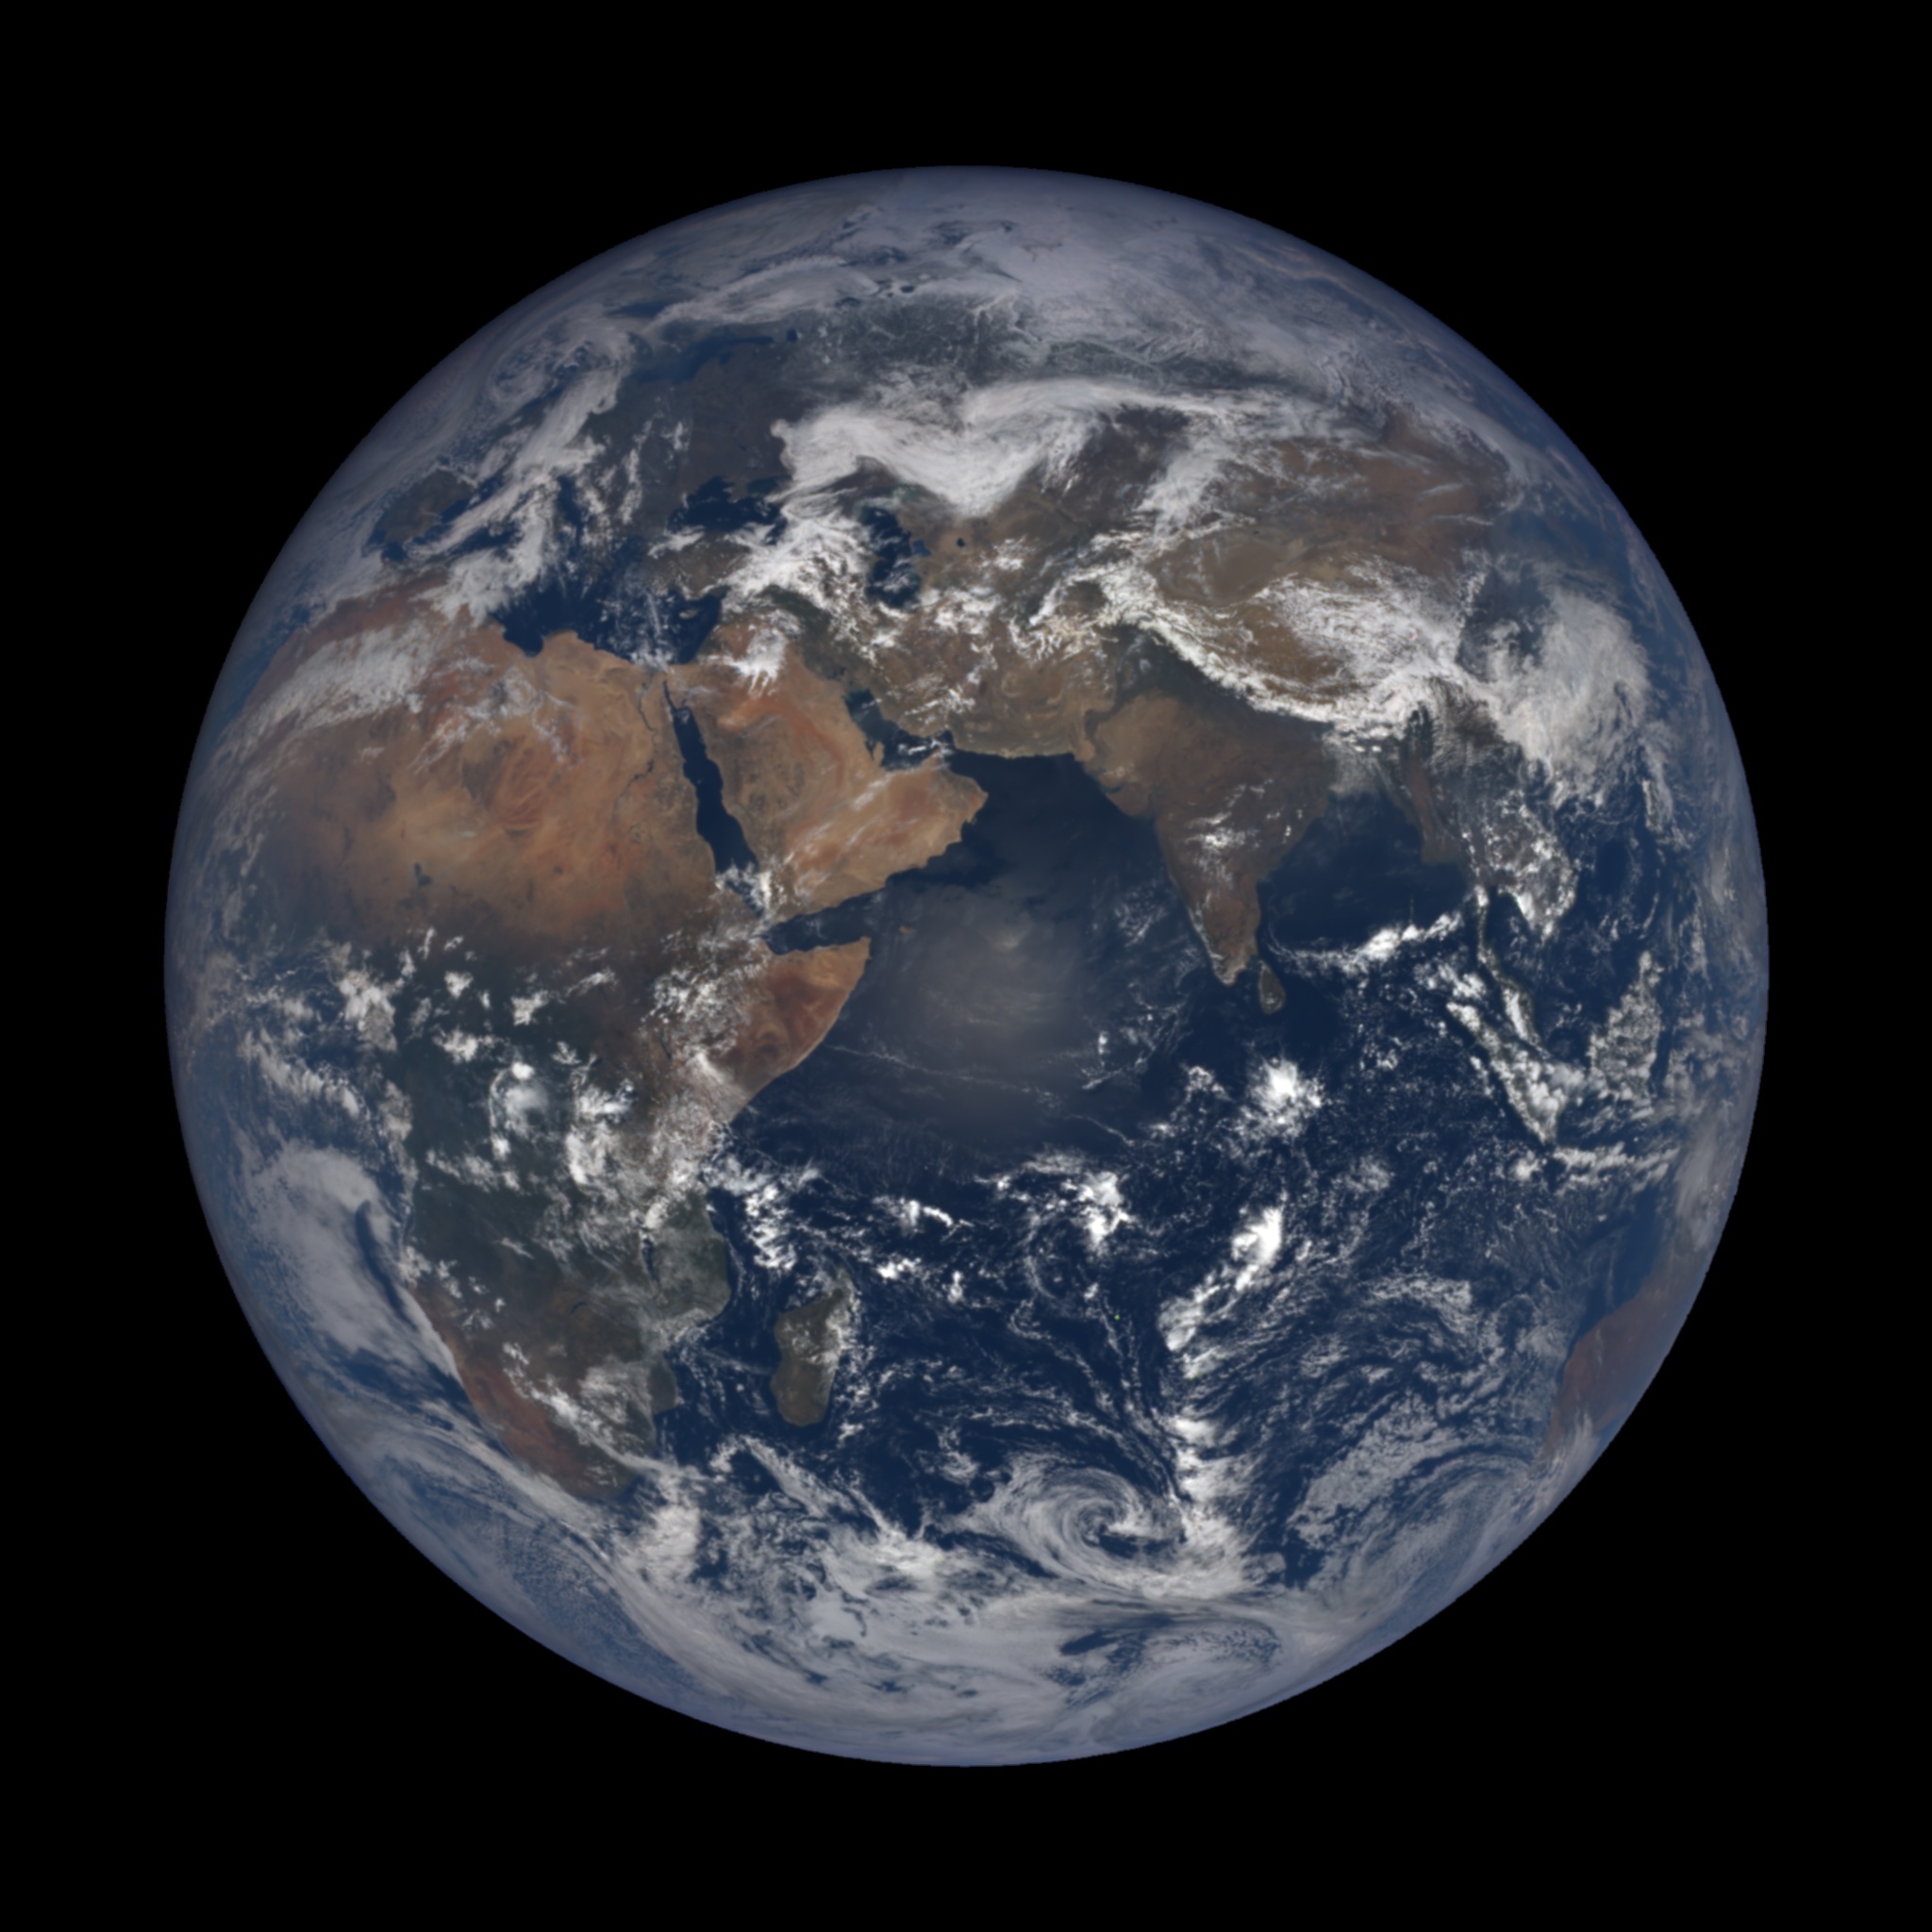
\includegraphics[width=5cm]{images/epic1}
%			\includegraphics[width=7cm]{images/fdl}
\end{columns}
\small\raggedleft(Large et al., 1954)
\end{center}

\vfill
\end{frame}
}

%\begin{frame}
%
%\frametitle{Photosynthesis}
%%	
%%	Photosynthesis
%
%\centering
%\begin{tikzpicture}
%\node(in){$6{\text{CO}}_{2}+6{\text{H}}_{2}\text{O}$};
%\node[right=of in, label={light absorbtion $\Delta \V{x}$}](arrow){$\to$};
%\node[right=of arrow]{${\text{C}}_{\text{6}}{\text{H}}_{\text{12}}{\text{O}}_{\text{6}}+{\text{6O}}_{\text{2}}$};
%\end{tikzpicture}
%%	
%%	\begin{equation*}
%%	6{\text{CO}}_{2}+6{\text{H}}_{2}\text{O}\to 
%%	\end{equation*}
%\end{frame}

\newcommand{\rastergrid}{
\begin{tikzpicture}
% each layer
\begin{scope}[scale=2]

% raster size
\def\d{0.7}		

% distance layer
\def\s{\d*5}

\foreach \i in {1,...,6}
{		
\begin{scope}[
yshift=\s*\i,every node/.append style={
yslant=0.5,xslant=-1},yslant=0.5,xslant=-1
]
%\draw[step=3.33mm] (0,0) grid (1,1);
%\fill[black,fill opacity=.9] (0.333,0.333) rectangle (0.333,0.333);    	    	  

\foreach \row in {0,...,2}{
\foreach \col in {0,...,2}{
\draw[tumblack, fill=tumblue!\pdfuniformdeviate 40,fill opacity=1,rounded corners=1] (\col*\d/3,\row*\d/3) rectangle (\col*\d/3+\d/3, \row*\d/3+\d/3);
%                 \draw[black, fill=black!\pdfuniformdeviate 40,fill opacity=1,rounded corners=1] (\col*\d/3,\row*\d/3) rectangle (\col*\d/3+\d/3, \row*\d/3+\d/3);
}
}

%\draw[step=3.33mm] (0,0) grid (1,1);
%\fill[white,fill opacity=.9] (0,0) rectangle (1,1);
\end{scope}
}
\end{scope}
\end{tikzpicture}
}


%\begin{frame}
%\frametitle{Spectral Band}
%\end{frame}


\begin{frame}
\frametitle{Multi-temporal Vegetation Modeling}

\begin{columns}
\column{.5\textwidth}

\begin{tikzpicture}
\node[] at (0,0){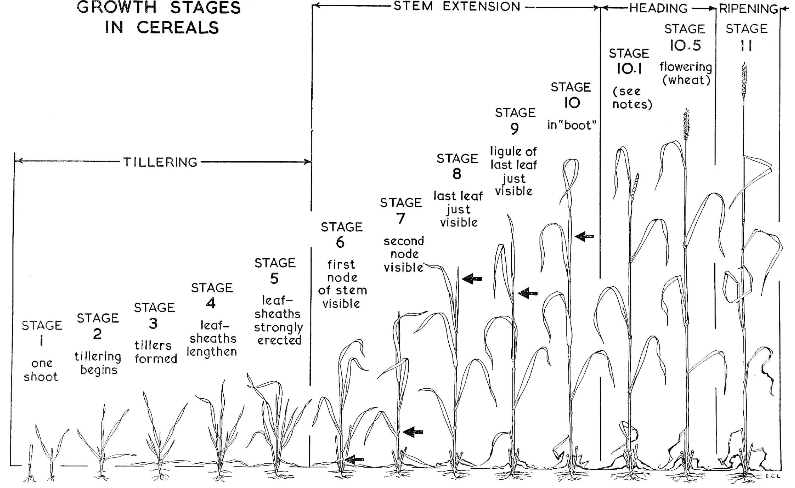
\includegraphics[width=\textwidth]{images/Large1954_cerial_growth_stages}};

%		\draw[step=1.0,black,thin, fill=none] (-2,-2) grid (2,2);

\visible<-1>{\draw [fill=white, draw=none, opacity=0.8] (-0.8,-3) rectangle (2,2.5);}
\visible<-2>{\draw [fill=white, draw=none, opacity=0.8] (2,-3) rectangle (5,2.5);}

\visible<1>{\node[rotate=190] at (-2.5,1.5){
\includegraphics[width=15mm]{images/icons/sat2}};}
\visible<2>{\node[rotate=225] at (-2.5,1.5){
\includegraphics[width=15mm]{images/icons/sat2}};}
\visible<3->{\node[rotate=260] at (-2.5,1.5){
\includegraphics[width=15mm]{images/icons/sat2}};}


\visible<4->{\node at (-1.5,1.4) {
\includegraphics[width=10mm]{images/cloud}};}

\end{tikzpicture}

\column{.5\textwidth}

{\Large
\only<1>{
\begin{equation*}
f_\text{vegetation}(\V{X}_t)
\end{equation*}
}
\only<2>{
\begin{equation*}
f_\text{vegetation}(\V{X}_t,\V{X}_{t+1})
\end{equation*}
}
\only<3>{
\begin{equation*}
f_\text{vegetation}(\V{X}_t,\V{X}_{t+1},\V{X}_{t+2})
\end{equation*}
}
}


\vspace{2em}


\visible<1->{
\includegraphics[width=.22\textwidth]{images/s2grid/1}}
\visible<2->{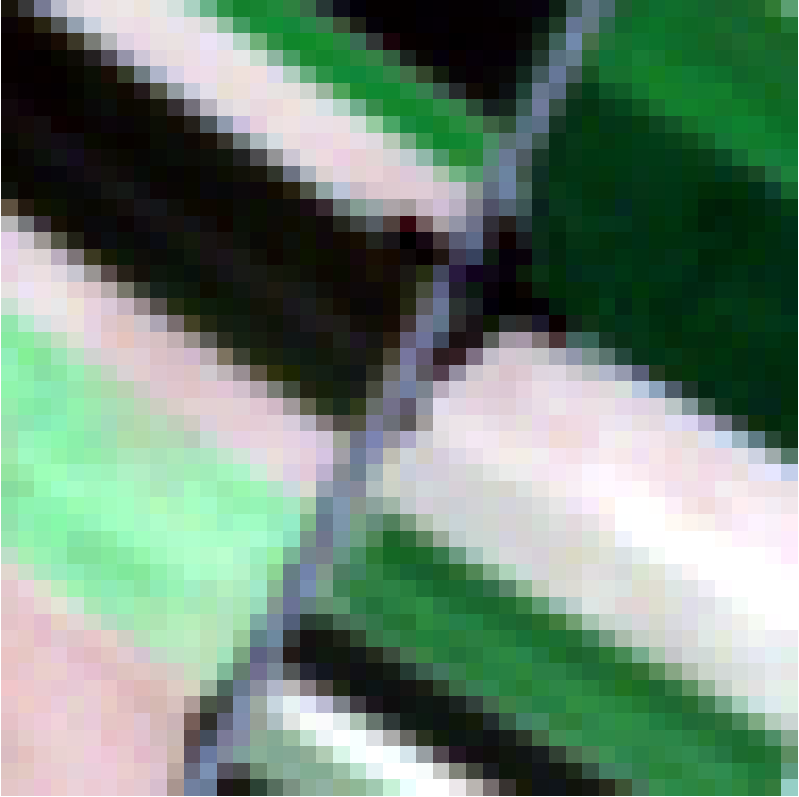
\includegraphics[width=.22\textwidth]{images/s2grid/2}}
\visible<3->{
\includegraphics[width=.22\textwidth]{images/s2grid/3}}
\visible<4->{
\includegraphics[width=.22\textwidth]{images/s2grid/4}}

\vspace{1em}

{\small 
Large, E. C. (1954). Growth stages in cereals illustration of the Feekes scale. Plant pathology, 3(4), 128-129.
}


\end{columns}
\end{frame}


\begin{frame}
\frametitle{Problem Definition}
\Large


\centering\begin{tikzpicture}[node distance=0em]
\visible<2->{\node(y){\V{y}};}
\visible<2->{\node[right=of y](equals){$=$};}
\node[right=of equals](f){$f_\text{vegetation}$};
\visible<1->{\node[right=of f](x){$(\V{X}_t,\V{X}_{t+1},\V{X}_{t+2})$};}

\end{tikzpicture}

\vspace{1em}
\raggedright

\begin{description}\setlength\itemsep{1em}
	\item[\color{tumblue}Problem:]<1-> \textbf{un/self-supervised learning} of a vegetation model \textbf{is difficult}
	\item[\color{tumblue}Solution:]<2-> re-framing as \textbf{supervised classification} of crop type labels
	\item[\color{tumblue}Intuition:]<3-> A \textbf{supervised classification model} must \textbf{internalize} a learned \textbf{discriminative model} for the \textbf{vegetation}
\end{description}

\end{frame}


\begin{frame}
\frametitle{Multi-temporal Earth observation}
\centering
\begin{tikzpicture}[scale=2]
%\draw[fill=tumblue, draw=none, opacity=0.5](-1,0) circle (1.5);
\node[fill=tumgraylight, draw=none, opacity=0.5, circle, minimum width=6cm, label=Earth Observation] at (-1,0){};

\node[fill=tumgraylight, draw=none, opacity=0.5, circle, minimum width=6cm, label=Machine Learning] at (1,0){};

\visible<1->{
	\node[font=\bfseries, circle, fill=tumbluelight, text width=2.5cm] (vhr) at (-1.5,.7) {high spatial \\ resolution};
	\node[font=\bfseries, circle, fill=tumorange!50, text width=2.5cm] (cv) at (1.5,.7) {computer vision methods};
	\draw[stealth-stealth, very thick] (vhr) -- node[midway,above]{well established} (cv);
}

\visible<2->{
	\node[font=\bfseries, circle, fill=tumbluelight, text width=2.5cm] (mt) at (-1.5,-.7) {high temporal resolution};
	\node[font=\bfseries, circle, fill=tumorange!50, text width=2.5cm] (nlp) at (1.5,-.7) {natural \\ language \\ processing};
	\draw[stealth-stealth, dotted] (mt) -- node[midway,above]{hardly anyone} (nlp);
}

\visible<3->{
	\node[fit=(nlp)(mt), draw, inner sep=.5em, rounded corners, thick, label=above:{\bfseries \Large my focus}]{};
}
%\draw[-stealth] (cv) -- (0,0);

%\draw[-stealth, very thick] (phd) -- (0,, fil0);
\end{tikzpicture}

\end{frame}

\begin{frame}
\frametitle{Example Analogy to Natural Language Processing}
\setrand{0}{100}{0.01}{1}
	\newcommand{\drawmatrix}{
		\left(\begin{matrix}\nextrand\thisrand\\\nextrand\thisrand\\\nextrand\thisrand\end{matrix}\right)
	}

	\newcommand{\image}[1]{
		\begin{tikzpicture}
			\node(img){\includegraphics[width=2cm]{#1}};
			\node[minimum width=.5em,minimum height=.5em, fill=tumbluelight, xshift=-1em] at (img)(rect){};
			
			\node[right=of rect, fill=tumbluelight,, inner sep=.2em, rounded corners=1em,  opacity=.2](m){$\drawmatrix$};
			\draw[tumbluelight] (rect.north) -- (m.north);
			\draw[tumbluelight] (rect.south) -- (m.south);
		\end{tikzpicture}
	}

	
	\begin{tikzpicture}[node distance=1em]
		\node[font=\scriptsize](e1){\image{images/analogy_examples/170127_snow.png}};
		\node[right=of e1, font=\scriptsize](e2){\image{images/analogy_examples/160929_clear.png}};
		\node[right=of e2, font=\scriptsize](e3){\image{images/analogy_examples/161115_cloudy.png}};
		\node[right=of e3, font=\scriptsize](e4){\image{images/analogy_examples/160728_partlycloudy.png}};
		
		\node[below=of e1, font=\scriptsize](t1){$E(\text{\textbf{The}})=\drawmatrix$};
		\node[below=of e2, font=\scriptsize](t2){$E(\text{\textbf{eagle}})=\drawmatrix$};
		\node[below=of e3, font=\scriptsize](t3){$E(\text{\textbf{has}})=\drawmatrix$};
		\node[below=of e4, font=\scriptsize](t4){$E(\text{\textbf{landed}})=\drawmatrix$};
		
		\node[above=of e1](x1){$\V{x}_1$};
		\node[above=of e2](x2){$\V{x}_2$};
		\node[above=of e3](x3){$\V{x}_3$};
		\node[above=of e4](x4){$\V{x}_4$};
		
		\node[right= 7em of e4](eo){$f(\M{X})$};
		\node[right= 7em of t4](nlp){$f(\M{X})$};
		
		\draw[-stealth] (e4) -- node[midway,above]{EO model} (eo);
		\draw[-stealth] (t4) -- node[midway,above]{NLP model} (nlp);
	\end{tikzpicture}
\end{frame}


%
%\begin{frame}
%\frametitle{Between two fields}
%\centering
%\begin{tikzpicture}[scale=2]
%%\draw[fill=tumblue, draw=none, opacity=0.5](-1,0) circle (1.5);
%\node[fill=tumbluelight, draw=none, opacity=0.5, circle, minimum width=6cm, label=Earth Observation] at (-1,0){};
%
%\node[fill=tumorange!50, draw=none, opacity=0.5, circle, minimum width=6cm, label=Machine Learning] at (1,0){};
%%\draw[fill=tumorange, draw=none, opacity=0.5](1,0) circle (1.5);
%
%\draw[-stealth, shorten >=1cm] (-1.3,1) -- (0,0);
%\draw[-stealth, shorten >=1cm] (-1.6,-1) -- (0,0);
%\draw[-stealth, shorten >=1cm] (-1.2,-.6) -- (0,0);
%\draw[-stealth, shorten >=1cm] (-1.8,.4) -- (0,0);
%\draw[-stealth, shorten >=1cm] (-1.3,.2) -- (0,0);
%
%\node[font=\bfseries] at (-2,0) {applications};
%
%\draw[-stealth, shorten >=1cm] (1.3,1) -- (0,0);
%\draw[-stealth, shorten >=1cm] (1.6,-1) -- (0,0);
%\draw[-stealth, shorten >=1cm] (1.2,-.6) -- (0,0);
%\draw[-stealth, shorten >=1cm] (1.8,.4) -- (0,0);
%\draw[-stealth, shorten >=1cm] (1.3,.2) -- (0,0);
%
%\node[font=\bfseries] at (2,0) {methods};
%
%\node[text width=2cm, circle, fill=tumblue, text=white]{global scale};
%
%\node[text width=2cm, circle, fill=tumblue, text=white]{global scale};
%
%\node[font=\normalsize, fill=white, text width=2cm, rounded corners, fill opacity=.5, text opacity=1](phd) at (0,0){global scaleability \\ real world impact \\ Open Data};
%
%%\draw[-stealth, very thick] (phd) -- (0,, fil0);
%\end{tikzpicture}
%
%
%\end{frame}


%



%
%
%\begin{frame}
%	\frametitle{Natural Language Processing}
%	
%	GPT-2 
%%	\cite{radford2019language}
%	
%	Bert Model Pretraining
%%	\cite{Devlin2018bert}
%	
%	
%\end{frame}



%\tikzsetnextfilename{input}

\newcommand{\timeseries}[1]{
\begin{tikzpicture}[baseline=-.25em]
	
	\tikzstyle{annot} = [font=\small\sffamily, text=tumblue]
	\tikzstyle{point} = [thin, tumbluelight, shorten >= .25em, shorten <= .25em]
	
	% from /home/marc/projects/EV2019/images/example/tstop.txt
%	\def\tstopv{0.6285714285714286}
	\def\class{winter barley}
	
	\begin{groupplot}[
	group style={
		group name=my plots,
		group size=1 by 1,
		columns=1,
		xlabels at=edge bottom,
		xticklabels at=edge bottom,
		vertical sep=1em,
	},
	ylabel near ticks,
	ylabel style={font=\sffamily\small, rotate=-90},
	width=.75\textwidth,
	height=3.8cm,
	axis x line=bottom,
	axis y line=left,
	enlarge x limits=0.01,
	xtick={0,0.25,0.5,0.75,1},
	xticklabels={Januar,April,Juni,September,Dezember},
	ymajorgrids,
	ymin=0, ymax=1.4
	]
	
	
	
	\nextgroupplot[
		no marks,  
		ylabel={},
		draw opacity=.8,
		smooth=0.01,
		legend columns=2,
		legend style={at={(.5,1.1)},anchor=south, line width=1pt, fill=tumblue!10}
		]
		 
	\addplot[b1color] table [x=t, y=B1, col sep=comma, forget plot] {images/example/#1};
	\addplot[b9color] table [x=t, y=B9, col sep=comma, forget plot] {images/example/#1};
	\addplot[b10color] table [x=t, y=B10, col sep=comma] {images/example/input.csv};
	
	\addplot[b11color] table [x=t, y=B11, col sep=comma, forget plot] {images/example/#1};
	\addplot[b12color] table [x=t, y=B12, col sep=comma] {images/example/#1};
	
	\addplot[b5color] table [x=t, y=B5, col sep=comma, forget plot] {images/example/#1};
	\addplot[b6color] table [x=t, y=B6, col sep=comma, forget plot] {images/example/#1};
	\addplot[b7color] table [x=t, y=B7, col sep=comma, forget plot] {images/example/#1};
	\addplot[b8color] table [x=t, y=B8, col sep=comma, forget plot] {images/example/#1};
	\addplot[b8Acolor] table [x=t, y=B8A, col sep=comma] {images/example/#1};
		
	\addplot[b2color] table [x=t, y=B2, col sep=comma, forget plot] {images/example/#1};
	\addplot[b3color] table [x=t, y=B3, col sep=comma, forget plot] {images/example/#1};
	\addplot[b4color] table [x=t, y=B4, col sep=comma] {images/example/#1};
%	
	\legend{3 atmospheric, 2 short-wave infrared, 5 near infrared, 3 visible bands}
	
%	\addplot[thick,colorclassone, name path=y1] table[x=t, y=y1]{\mydata};
%	\addplot[thick,colorclasstwo, name path=y2] table[x=t, y=y2]{\mydata};
%	\addplot[thick,colorclassthree, name path=y3] table[x=t, y=y3]{\mydata};
%	\addplot[thick,colorclassfour, name path=y4] table[x=t, y=y4]{\mydata};
	%\addplot[colorblue!20] fill between[of = y1 and axis];
	%\addplot[colorhgray!20] fill between[of = y2 and axis];
	%\addplot[colorgreen!20] fill between[of = y3 and axis];
	%\addplot[colororange!20] fill between[of = y4 and axis];
	
	
	\end{groupplot}
	
	\end{tikzpicture}
}


\begin{frame}
\frametitle{Multi-temporal Vegetation Monitoring}

\begin{columns}
	\column{.5\textwidth}
	
	\begin{tikzpicture}
		\node[] at (0,0){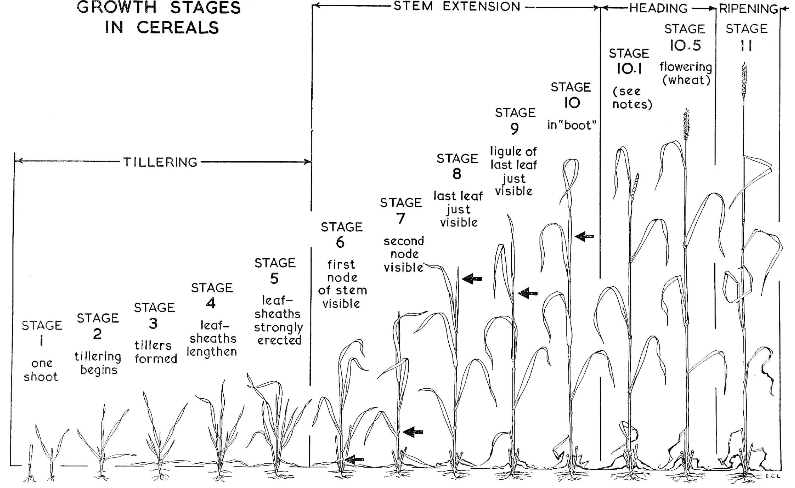
\includegraphics[width=\textwidth]{images/Large1954_cerial_growth_stages}};
		
%		\draw[step=1.0,black,thin, fill=none] (-2,-2) grid (2,2);
		
		\visible<-1>{\draw [fill=white, draw=none, opacity=0.8] (-0.8,-3) rectangle (2,2.5);}
		\visible<-2>{\draw [fill=white, draw=none, opacity=0.8] (2,-3) rectangle (5,2.5);}
		
		\visible<1>{\node[rotate=190] at (-2.5,1.5){
\includegraphics[width=15mm]{images/icons/sat2}};}
		\visible<2>{\node[rotate=225] at (-2.5,1.5){
\includegraphics[width=15mm]{images/icons/sat2}};}
		\visible<3->{\node[rotate=260] at (-2.5,1.5){
\includegraphics[width=15mm]{images/icons/sat2}};}
		
		
		\visible<4->{\node at (-1.5,1.4) {
\includegraphics[width=10mm]{images/cloud}};
		}
		
	\end{tikzpicture}
	
	\column{.5\textwidth}
	
	{\Large
	\only<1>{
	\begin{equation*}
		\V{y} = f_\text{phenology}(\V{X}_t)
	\end{equation*}
	}
	\only<2>{
		\begin{equation*}
		\V{y} = f_\text{phenology}(\V{X}_t,\V{X}_{t+1})
		\end{equation*}
	}
	\only<3>{
		\begin{equation*}
		\V{y} = f_\text{phenology}(\V{X}_t,\V{X}_{t+1},\V{X}_{t+2})
		\end{equation*}
	}
	}
	
	
	\vspace{2em}

	
	\visible<1->{
\includegraphics[width=.22\textwidth]{images/s2grid/1}}
	\visible<2->{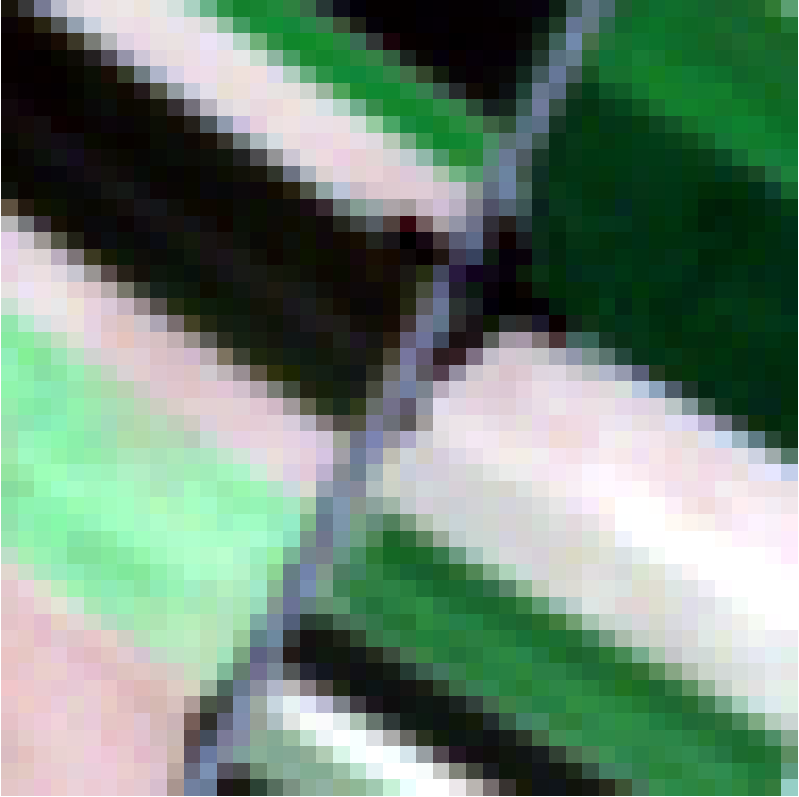
\includegraphics[width=.22\textwidth]{images/s2grid/2}}
	\visible<3->{
\includegraphics[width=.22\textwidth]{images/s2grid/3}}
	\visible<4->{\includegraphics[width=.22\textwidth]{images/s2grid/4}}
	
	\vspace{1em}
	
	{\small 
		Large, E. C. (1954). Growth stages in cereals illustration of the Feekes scale. Plant pathology, 3(4), 128-129.
	}
	
	
\end{columns}



\end{frame}



\begin{frame}[t]
\frametitle{Looking at Sequence to Sequence Models from NLP}
%	\framesubtitle{Natürlicher Sprachverarbeitung, Übersetzung, Spracherkennung}

%Verbreitet in sequenziellen Aufgabengebieten, wie natürlicher Sprachverarbeitung, Übersetzung, Spracherkennung
%	\begin{center}
%		\large Wort-Sequenz $\rightarrow$ Representation $c$ $\rightarrow$ Wort-Sequenz
%	\end{center}
\begin{center}
	%\tikzsetnextfilename{seq2seq}

\tikzstyle{operator} = [draw, circle, fill=tumbluemedium, draw=tumbluemedium, inner sep=0, text=white]
%\tikzstyle{function} = [draw, rectangle, fill=tumbluemedium, draw=tumbluemedium, text=white]
\tikzstyle{gate} = [fill=tumivory,draw,rounded corners]

\tikzstyle{dummy} = [inner sep=0]
\tikzstyle{flow} = [rounded corners]
\tikzstyle{endflow} = [-stealth,flow]
\tikzstyle{beginflow} = [stealth-,flow]

\tikzstyle{bigbox} = [rectangle, draw=tumivory, thick, fill=tumgraylight, rounded corners, 
inner sep=.5ex]

\tikzstyle{bigpassbox} = [opacity=.2, rounded corners, draw=none]


\tikzset{pic shift/.store in=\shiftcoord,
	pic shift={(0,0)},
	pics/seqlstmencoder/.style={
		code={
		\begin{scope}[shift={\shiftcoord},xscale=1.3,yscale=.9]
			
			\node[dummy] (bl) at (0,0){}; % bottom left
			\node[dummy] (tr) at (1,1){}; % top right
			
			\node[dummy] (br) at ($ (bl -| tr) $){}; % bottom right
			\node[dummy] (tl) at ($ (bl |- tr) $){}; % top left
			
			\node[fit=(bl) (tr),bigbox] (-C) {};
			
			% input coordinate for rounded draw lines -> slightly right of tl
			\coordinate (-input) at (0.1,1); % top left
			
			% output coordinate for rounded draw lines -> slightly left of br
			\coordinate (-coutput) at (0.9,0); % bottom right
			\coordinate (-cinput) at (0.1,0); % bottom left
			\coordinate (-houtput) at (0.9,1); % bottom right
			
%			% gate distance
			\def\d{1/6}
			
			% gate heights
			\def\h{1/3}
			
			\coordinate (f)  at bl+(1*\d,0);
			\coordinate (i)  at bl+(2*\d,0);
			\coordinate (j)  at bl+(3*\d,0);
			\coordinate (o)  at bl+(4*\d,0);
			\coordinate (out) at bl+(5*\d,0);
			
			\coordinate (gates) at (0,2*\h);
			
			%\node[above=of tl](xt){$x_{t}$};
			%\node[left=of tl](htminus1){$h_{t-1}$};
			
			%\node[below=of br](ct){$c_{t}$};
			
			\node[gate](fgate) at ($ (gates -| f) $){};
			\node[gate](igate) at ($ (gates -| i) $){};
			\node[gate](jgate) at ($ (gates -| j) $){};
			\node[gate](ogate) at ($ (gates -| o) $){};
			
%			\coordinate (htminus1) at bl+(-.5,0);
%			\coordinate (ht) at bl+(-.5,0);
%			
			% forget gate
			\node[operator](fmult) at ($ (bl -| fgate) $) {};
			\draw[endflow] (-input) -| (fgate) -- (fmult); 
			
%			%j
			\node[operator](jmult) at ([shift={(0,-1*\h)}]jgate) {};
			\node[operator](cadd) at ($ (bl -| jgate) $) {};
			\draw[endflow] (-input) -| (jgate) -- (jmult);
			\draw[endflow] (jmult) -- (cadd); 			

%			%i	
			\draw[endflow] (-input) -| (igate) |- (jmult); 
%
%%			% outpu
			\node[operator](outtanh) at ([shift={(0,1*\h)}]out) {};
%			
%			%o 
			\draw[endflow] (tl) -| (ogate) |- (outtanh);
			\draw[flow] (outtanh) |- (-houtput);
%			
%			% output flow
			\draw[endflow] (cadd) -| (outtanh);
			\draw[flow] (-cinput) -- (fmult) -- (cadd) -- (-coutput);
%			
			
			% debug
%			\node at (gates) {\tiny{gates}};
%			\node at (-input) {\tiny{-input}};
%			\node at (-coutput) {\tiny{-coutput}};
%			\node at (-houtput) {\tiny{-houtput}};
%			\node at (f) {\tiny{f}};
%			\node at (i) {\tiny{i}};
%			\node at (j) {\tiny{j}};
%			\node at (o) {\tiny{o}};
%			\node at (tl) {\tiny{tl}};
%			\node at (br) {\tiny{br}};
%			\node at (bl) {\tiny{bl}};
%			\node at (tr) {\tiny{tr}};
%			\node at (out) {\tiny{out}};
			
		\end{scope}
		}
	}
}
\tikzset{pic shift/.store in=\shiftcoord,
	pic shift={(0,0)},
	pics/seqlstmdecoder/.style={
		code={
			\begin{scope}[shift={\shiftcoord},xscale=1.3,yscale=-.9]
				
				\node[dummy] (bl) at (0,0){}; % bottom left
				\node[dummy] (tr) at (1,1){}; % top right
				
				\node[dummy] (br) at ($ (bl -| tr) $){}; % bottom right
				\node[dummy] (tl) at ($ (bl |- tr) $){}; % top left
				
				\node[fit=(bl) (tr),bigbox] (-C) {};
				
				% input coordinate for rounded draw lines -> slightly right of tl
				\coordinate (-input) at (0.1,1); % top left
				
				% output coordinate for rounded draw lines -> slightly left of br
				\coordinate (-coutput) at (0.9,0); % bottom right
				\coordinate (-cinput) at (0.1,0); % bottom left
				\coordinate (-houtput) at (0.9,1); % top right
				
				%			% gate distance
				\def\d{1/6}
				
				% gate heights
				\def\h{1/3}
				
				\coordinate (f)  at bl+(1*\d,0);
				\coordinate (i)  at bl+(2*\d,0);
				\coordinate (j)  at bl+(3*\d,0);
				\coordinate (o)  at bl+(4*\d,0);
				\coordinate (out) at bl+(5*\d,0);
				
				\coordinate (gates) at (0,2*\h);
				
				%\node[above=of tl](xt){$x_{t}$};
				%\node[left=of tl](htminus1){$h_{t-1}$};
				
				%\node[below=of br](ct){$c_{t}$};
				
				\node[gate](fgate) at ($ (gates -| f) $){};
				\node[gate](igate) at ($ (gates -| i) $){};
				\node[gate](jgate) at ($ (gates -| j) $){};
				\node[gate](ogate) at ($ (gates -| o) $){};
				
				%			\coordinate (htminus1) at bl+(-.5,0);
				%			\coordinate (ht) at bl+(-.5,0);
				%			
				% forget gate
				\node[operator](fmult) at ($ (bl -| fgate) $) {};
				\draw[endflow] (-input) -| (fgate) -- (fmult); 
				
				%			%j
				\node[operator](jmult) at ([shift={(0,-1*\h)}]jgate) {};
				\node[operator](cadd) at ($ (bl -| jgate) $) {};
				\draw[endflow] (-input) -| (jgate) -- (jmult);
				\draw[endflow] (jmult) -- (cadd); 			
				
				%			%i	
				\draw[endflow] (-input) -| (igate) |- (jmult); 
				%
				%%			% outpu
				\node[operator](outtanh) at ([shift={(0,1*\h)}]out) {};
				%			
				%			%o 
				\draw[endflow] (tl) -| (ogate) |- (outtanh);
				\draw[flow] (outtanh) |- (-houtput);
				%			
				%			% output flow
				\draw[endflow] (cadd) -| (outtanh);
				\draw[flow] (-cinput) -- (fmult) -- (cadd) -- (-coutput);
				%			
				
				% debug
				%			\node at (gates) {\tiny{gates}};
				%			\node at (-input) {\tiny{-input}};
				%			\node at (-coutput) {\tiny{-coutput}};
				%			\node at (-houtput) {\tiny{-houtput}};
				%			\node at (f) {\tiny{f}};
				%			\node at (i) {\tiny{i}};
				%			\node at (j) {\tiny{j}};
				%			\node at (o) {\tiny{o}};
				%			\node at (tl) {\tiny{tl}};
				%			\node at (br) {\tiny{br}};
				%			\node at (bl) {\tiny{bl}};
				%			\node at (tr) {\tiny{tr}};
				%			\node at (out) {\tiny{out}};
				
			\end{scope}
		}
	}
}


\begin{tikzpicture}[scale=1, node distance=2em]%,show background rectangle,background rectangle/.style={draw=red}]

%\matrix (m) [matrix of nodes, ampersand replacement=\&]{

\def\d{1.8}
\def\encoderheight{0}
\def\decoderheight{-1.3}

\draw pic (enc1) at (\d,\encoderheight) {seqlstmencoder};% \&
\node[above=of enc1tl](xenc1){I};

\draw pic (enc2) at (2*\d,\encoderheight) {seqlstmencoder};
\node[above=of enc2-input](xenc2){live};

\draw pic (enc3) at (3*\d,\encoderheight) {seqlstmencoder};
\node[above=of enc3-input](xenc3){in};

\draw pic (enc4) at (4*\d,\encoderheight) {seqlstmencoder};
\node[above=of enc4-input](xenc4){Munich};

\draw pic (dec1) at (1*\d,\decoderheight) {seqlstmdecoder};% \&
\node[below=of dec1tr](ydec1){Ich};

\draw pic (dec2) at (2*\d,\decoderheight) {seqlstmdecoder};
\node[below=of dec2tr](ydec2){lebe};

\draw pic (dec3) at (3*\d,\decoderheight) {seqlstmdecoder};
\node[below=of dec3tr](ydec3){in};

\draw pic (dec4) at (4*\d,\decoderheight) {seqlstmdecoder};
\node[below=of dec4tr](ydec4){München};

\node[anchor=center](state) at ($(enc4-coutput)!0.5!(dec1-cinput)$){representation $\VCellState_T$};

\node[left=of enc1-input](enczerostateh){$\V{0}$};
\node[left=of enc1-cinput](enczerostatec){$\V{0}$};
\node[left=of dec1-input](deczerostateh){$\V{0}$};

\draw[endflow] (enczerostateh) -- (enc1-input);
\draw[endflow] (enczerostatec) -- (enc1-cinput);
\draw[endflow] (deczerostateh) -- (dec1-input);


% draw state
\draw[flow] (enc4-coutput) -- ++(.2,0) |- (state);
\draw[beginflow] (dec1-cinput) -- ++(-.2,0) |- (state);

% draw connections from input to cells
\draw[flow] (xenc1) |- (enc1-input);
\draw[flow] (xenc2) |- (enc2-input);
\draw[flow] (xenc3) |- (enc3-input);
\draw[flow] (xenc4) |- (enc4-input);

% draw connections from cells to output
\draw[beginflow] (ydec1) |- (dec1-houtput);
\draw[beginflow] (ydec2) |- (dec2-houtput);
\draw[beginflow] (ydec3) |- (dec3-houtput);
\draw[flow] (ydec4) |- (dec4-houtput);

% draw hidden connections between cells
\draw[endflow] (enc1-houtput) -- (enc2-input);
\draw[endflow] (enc2-houtput) -- (enc3-input);
\draw[endflow] (enc3-houtput) -- (enc4-input);

\draw[endflow] (dec1-houtput) -- (dec2-input);
\draw[endflow] (dec2-houtput) -- (dec3-input);
\draw[endflow] (dec3-houtput) -- (dec4-input);

% draw hidden connections between cells
\draw[endflow] (enc1-coutput) -- (enc2-cinput);
\draw[endflow] (enc2-coutput) -- (enc3-cinput);
\draw[endflow] (enc3-coutput) -- (enc4-cinput);

\draw[endflow] (dec1-coutput) -- (dec2-cinput);
\draw[endflow] (dec2-coutput) -- (dec3-cinput);
\draw[endflow] (dec3-coutput) -- (dec4-cinput);

%\node[bigpassbox, fill=classcolor, rectangle, minimum width=4cm,minimum height=3.5cm, anchor=center, label={[shift={(-1ex,-3.5ex)}]north:classification}] (classbox) at (13,0) {};
%};

\end{tikzpicture}
\end{center}
%\begin{columns}
%	\column{.4\textwidth}
%	%		\brand{Word2Vec} embedding 
%	%		Neural Machine Translation encodes 
%	
%	\centering 
%%	
%%	\begin{tikzpicture}
%%	\node[fill=tumbluelight!50,rounded corners](x){Eingabesequenz};
%%	\node[fill=tumbluelight!50,rounded corners, below=of x](c){Repräsentation};
%%	\node[fill=tumbluelight!50,rounded corners, below=of c](o){Ausgabsequenz};
%%	
%%	\draw[-stealth] (x) -- (c);
%%	\draw[-stealth] (c) -- (o);
%%	
%%	\end{tikzpicture}
%%	
%	\column{.6\textwidth}
%	
%\end{columns}


{\small
	Sutskever, I., Vinyals, O., \& Le, Q. V. (2014). Sequence to sequence learning with neural networks. In Advances in neural information processing systems (pp. 3104-3112).}


\end{frame}

%\tikzsetnextfilename{network}

\tikzstyle{operator} = [draw, circle, fill=tumbluemedium, draw=tumbluemedium, inner sep=0, text=white]
%\tikzstyle{function} = [draw, rectangle, fill=tumbluemedium, draw=tumbluemedium, text=white]
\tikzstyle{gate} = [fill=tumivory,draw,rounded corners]

\tikzstyle{dummy} = [inner sep=0]
\tikzstyle{flow} = [rounded corners]
\tikzstyle{endflow} = [-stealth,flow]
\tikzstyle{beginflow} = [stealth-,flow]

\tikzstyle{bigpassbox} = [opacity=.2, rounded corners, draw=none]

% defaultvalue -> might be replaced later
\colorlet{tensorcolor}{tumblue}

\tikzstyle{bigbox} = [rectangle, draw=tumivory, thick, fill=tumgraylight, rounded corners, 
inner sep=.5ex]

\tikzstyle{wireframe} = [draw=tumgray]
\tikzstyle{image} = [inner sep=0, fill=none, minimum size=\imagewidth]

\tikzset{pic shift/.store in=\shiftcoord,
	pic shift={(0,0)},
	pics/seqlstmfw/.style={
		code={
		\begin{scope}[shift={\shiftcoord},xscale=1.3,yscale=.8]
			
			\node[dummy] (bl) at (0,0){}; % bottom left
			\node[dummy] (tr) at (1,1){}; % top right
			
			\node[dummy] (br) at ($ (bl -| tr) $){}; % bottom right
			\node[dummy] (tl) at ($ (bl |- tr) $){}; % top left
			
			\node[fit=(bl) (tr),bigbox] (-C) {};
			
			% input coordinate for rounded draw lines -> slightly right of tl
			\coordinate (-input) at (0.1,1); % top left
			
			% output coordinate for rounded draw lines -> slightly left of br
			\coordinate (-coutput) at (0.9,0); % bottom right
			\coordinate (-cinput) at (0.1,0); % bottom left
			\coordinate (-houtput) at (0.9,1); % bottom right
			
%			% gate distance
			\def\d{1/6}
			
			% gate heights
			\def\h{1/3}
			
			\coordinate (f)  at bl+(1*\d,0);
			\coordinate (i)  at bl+(2*\d,0);
			\coordinate (j)  at bl+(3*\d,0);
			\coordinate (o)  at bl+(4*\d,0);
			\coordinate (out) at bl+(5*\d,0);
			
			\coordinate (gates) at (0,2*\h);
			
			%\node[above=of tl](xt){$x_{t}$};
			%\node[left=of tl](htminus1){$h_{t-1}$};
			
			%\node[below=of br](ct){$c_{t}$};
			
			\node[gate](fgate) at ($ (gates -| f) $){};
			\node[gate](igate) at ($ (gates -| i) $){};
			\node[gate](jgate) at ($ (gates -| j) $){};
			\node[gate](ogate) at ($ (gates -| o) $){};
			
%			\coordinate (htminus1) at bl+(-.5,0);
%			\coordinate (ht) at bl+(-.5,0);
%			
			% forget gate
			\node[operator](fmult) at ($ (bl -| fgate) $) {};
			\draw[endflow] (-input) -| (fgate) -- (fmult); 
			
%			%j
			\node[operator](jmult) at ([shift={(0,-1*\h)}]jgate) {};
			\node[operator](cadd) at ($ (bl -| jgate) $) {};
			\draw[endflow] (-input) -| (jgate) -- (jmult);
			\draw[endflow] (jmult) -- (cadd); 			

%			%i	
			\draw[endflow] (-input) -| (igate) |- (jmult); 
%
%%			% outpu
			\node[operator](outtanh) at ([shift={(0,1*\h)}]out) {};
%			
%			%o 
			\draw[endflow] (tl) -| (ogate) |- (outtanh);
			\draw[flow] (outtanh) |- (-houtput);
%			
%			% output flow
			\draw[endflow] (cadd) -| (outtanh);
			\draw[flow] (-cinput) -- (fmult) -- (cadd) -- (-coutput);
%			
			
			% debug
%			\node at (gates) {\tiny{gates}};
%			\node at (-input) {\tiny{-input}};
%			\node at (-coutput) {\tiny{-coutput}};
%			\node at (-houtput) {\tiny{-houtput}};
%			\node at (f) {\tiny{f}};
%			\node at (i) {\tiny{i}};
%			\node at (j) {\tiny{j}};
%			\node at (o) {\tiny{o}};
%			\node at (tl) {\tiny{tl}};
%			\node at (br) {\tiny{br}};
%			\node at (bl) {\tiny{bl}};
%			\node at (tr) {\tiny{tr}};
%			\node at (out) {\tiny{out}};
			
		\end{scope}
		}
	}
}

\tikzset{pic shift/.store in=\shiftcoord,
	pic shift={(0,0)},
	pics/seqlstmbw/.style={
		code={
			\begin{scope}[shift={\shiftcoord},xscale=1.3,yscale=-.8]
				
				\node[dummy] (bl) at (0,0){}; % bottom left
				\node[dummy] (tr) at (1,1){}; % top right
				
				\node[dummy] (br) at ($ (bl -| tr) $){}; % bottom right
				\node[dummy] (tl) at ($ (bl |- tr) $){}; % top left
				
				\node[fit=(bl) (tr),bigbox] (-C) {};
				
				% input coordinate for rounded draw lines -> slightly right of tl
				\coordinate (-input) at (0.1,1); % top left
				
				% output coordinate for rounded draw lines -> slightly left of br
				\coordinate (-coutput) at (0.9,0); % bottom right
				\coordinate (-cinput) at (0.1,0); % bottom left
				\coordinate (-houtput) at (0.9,1); % top right
				
				%			% gate distance
				\def\d{1/6}
				
				% gate heights
				\def\h{1/3}
				
				\coordinate (f)  at bl+(1*\d,0);
				\coordinate (i)  at bl+(2*\d,0);
				\coordinate (j)  at bl+(3*\d,0);
				\coordinate (o)  at bl+(4*\d,0);
				\coordinate (out) at bl+(5*\d,0);
				
				\coordinate (gates) at (0,2*\h);
				
				%\node[above=of tl](xt){$x_{t}$};
				%\node[left=of tl](htminus1){$h_{t-1}$};
				
				%\node[below=of br](ct){$c_{t}$};
				
				\node[gate](fgate) at ($ (gates -| f) $){};
				\node[gate](igate) at ($ (gates -| i) $){};
				\node[gate](jgate) at ($ (gates -| j) $){};
				\node[gate](ogate) at ($ (gates -| o) $){};
				
				%			\coordinate (htminus1) at bl+(-.5,0);
				%			\coordinate (ht) at bl+(-.5,0);
				%			
				% forget gate
				\node[operator](fmult) at ($ (bl -| fgate) $) {};
				\draw[endflow] (-input) -| (fgate) -- (fmult); 
				
				%			%j
				\node[operator](jmult) at ([shift={(0,-1*\h)}]jgate) {};
				\node[operator](cadd) at ($ (bl -| jgate) $) {};
				\draw[endflow] (-input) -| (jgate) -- (jmult);
				\draw[endflow] (jmult) -- (cadd); 			
				
				%			%i	
				\draw[endflow] (-input) -| (igate) |- (jmult); 
				%
				%%			% outpu
				\node[operator](outtanh) at ([shift={(0,1*\h)}]out) {};
				%			
				%			%o 
				\draw[endflow] (tl) -| (ogate) |- (outtanh);
				\draw[flow] (outtanh) |- (-houtput);
				%			
				%			% output flow
				\draw[endflow] (cadd) -| (outtanh);
				\draw[flow] (-cinput) -- (fmult) -- (cadd) -- (-coutput);
				%			
				
				% debug
				%			\node at (gates) {\tiny{gates}};
				%			\node at (-input) {\tiny{-input}};
				%			\node at (-coutput) {\tiny{-coutput}};
				%			\node at (-houtput) {\tiny{-houtput}};
				%			\node at (f) {\tiny{f}};
				%			\node at (i) {\tiny{i}};
				%			\node at (j) {\tiny{j}};
				%			\node at (o) {\tiny{o}};
				%			\node at (tl) {\tiny{tl}};
				%			\node at (br) {\tiny{br}};
				%			\node at (bl) {\tiny{bl}};
				%			\node at (tr) {\tiny{tr}};
				%			\node at (out) {\tiny{out}};
				
			\end{scope}
		}
	}
}

%\newcommand{}{
%	\begin{tikzpicture}
%	% each layer
%	\begin{scope}[scale=2]
%	
%	% raster size
%	\def\d{0.7}		
%	
%	% distance layer
%	\def\s{\d*5}
%	
%	\foreach \i in {1,...,6}
%	{		
%		\begin{scope}[
%		yshift=\s*\i,every node/.append style={
%			yslant=0.5,xslant=-1},yslant=0.5,xslant=-1
%		]
%		%\draw[step=3.33mm] (0,0) grid (1,1);
%		%\fill[black,fill opacity=.9] (0.333,0.333) rectangle (0.333,0.333);    	    	  
%		
%		\foreach \row in {0,...,2}{
%			\foreach \col in {0,...,2}{
%				\draw[tumblack, fill=tumblue!\pdfuniformdeviate 40,fill opacity=1,rounded corners=1] (\col*\d/3,\row*\d/3) rectangle (\col*\d/3+\d/3, \row*\d/3+\d/3);
%				%                 \draw[black, fill=black!\pdfuniformdeviate 40,fill opacity=1,rounded corners=1] (\col*\d/3,\row*\d/3) rectangle (\col*\d/3+\d/3, \row*\d/3+\d/3);
%			}
%		}
%		
%		%\draw[step=3.33mm] (0,0) grid (1,1);
%		%\fill[white,fill opacity=.9] (0,0) rectangle (1,1);
%		\end{scope}
%	}
%	\end{scope}
%	\end{tikzpicture}
%}
%%
%\newcommand{}{
%	
%	\begin{tikzpicture}[scale=2]
%	\foreach \i in {0,...,9}
%	\draw[tumblack,fill=tumorange!\pdfuniformdeviate 40,fill opacity=.9, rounded corners=0.5] (\i*.2, 0) rectangle (\i*.2+.2, .2);
%	\end{tikzpicture}
%}

\newcommand{\figencoderfieldRNN}{
	
	\begin{tikzpicture}[scale=1, node distance=1em]%,show background rectangle,background rectangle/.style={draw=red}]
	
	%\matrix (m) [matrix of nodes, ampersand replacement=\&]{
	
	\def\d{1.7}
	\def\encoderheight{0.4}
	\def\decoderheight{-0.4}
	\def\imagewidth{8mm}
	\def\stateimagewidth{8mm}
	\def\classimagewidth{8mm}
	
	\def\rgbone{images/network/48px/rgb1}
	\def\rgbtwo{images/network/48px/rgb2}
	\def\rgbthree{images/network/48px/rgb3}
	\def\rgbfour{images/network/48px/rgb4}
	\def\prediction{images/network/48px/prediction}
	\def\groundtruth{images/network/48px/ground_truth}
	\def\activation{images/network/48px/maize}
	\def\state{images/network/48px/state}
	
	
	%\draw [bigpassbox, fill=forwardcolor](1,.25) rectangle (10,4);
	
	\node[bigpassbox, fill=none, rectangle, minimum width=7cm,minimum height=3cm, anchor=south west, label={[shift={(2em,-3.5ex)}]north:}] (forwardbox) at (1,.15) {};
	%\draw [bigpassbox, fill=backwardcolor](1,-.25) rectangle (10,-4);
	
	\draw pic (fw1) at (\d,\encoderheight) {seqlstmfw};% \&
	\node[above=of fw1tl, label=above:{$\VInput_{1}$}](xfw1){
		
	};%images/network/time1_x
	
	\node[below= 3.5emof fw1-houtput, xshift=.5em, label=below:{$\V{y}_{1}$}](yfw1){
		
	};%images/network/time1_x
	
	\draw pic (fw2) at (2*\d,\encoderheight) {seqlstmfw};
	\node[above=of fw2-input, label=above:{$\VInput_{2}$}](xfw2){
		
	}; % images/network/time11_x
	
	\node[below= 3.5emof fw2-houtput, xshift=.5em, label=below:{$\V{y}_{2}$}](yfw2){
		
	};%images/network/time1_x
	
	\draw pic (fw3) at (3*\d,\encoderheight) {seqlstmfw};
	\node[above=of fw3-input](xfw3){$\dots$};
	\node[below= 3.5emof fw3-houtput, xshift=.5em](yfw3){
		%	
		$\dots$
	};%images/network/time1_x
	
	\draw pic (fw4) at (4*\d,\encoderheight) {seqlstmfw};
	\node[above=of fw4-input, label=above:{$\VInput_T$}](xfw4){
		
	}; % images/network/time30_x
	
	\node[below= 3.5emof fw4-houtput, xshift=.5em, label=below:{$\V{y}_{T}$}](yfw4){
		
	};%images/network/time1_x
	
	\node[left=of fw1-input](enczerostateh){$\V{0}$};
	\node[left=of fw1-cinput](enczerostatec){$\V{0}$};
	\draw[endflow] (enczerostateh) -- (fw1-input);
	\draw[endflow] (enczerostatec) -- (fw1-cinput);
	
	% draw connections from input to cells
	\draw[flow] (xfw1) |- (fw1-input);
	\draw[flow] (xfw2) |- (fw2-input);
	\draw[flow] (xfw3) |- (fw3-input);
	\draw[flow] (xfw4) |- (fw4-input);
	
	% draw hidden connections between cells
	\draw[endflow] (fw1-houtput) -- (fw2-input);
	\draw[endflow] (fw2-houtput) -- (fw3-input);
	\draw[endflow] (fw3-houtput) -- (fw4-input);
	
	% draw hidden connections between cells
	\draw[endflow] (fw1-coutput) -- (fw2-cinput);
	\draw[endflow] (fw2-coutput) -- (fw3-cinput);
	\draw[endflow] (fw3-coutput) -- (fw4-cinput);
	
	% outputs
	\draw[endflow] (fw1-houtput) -- ($ (fw1-houtput)+(.5em,0) $) -- (yfw1);
	\draw[endflow] (fw2-houtput) -- ($ (fw2-houtput)+(.5em,0) $) -- (yfw2);
	\draw[endflow] (fw3-houtput) -- ($ (fw3-houtput)+(.5em,0) $) -- (yfw3);
	\draw[endflow] (fw4-houtput) -- ($ (fw4-houtput)+(.5em,0) $) -- (yfw4);
	
	%\node[right= 2.5em of fw4-coutput](cfw){$\VCellState_T^\text{fw}$};
	
	%\draw[endflow] (fw4-coutput) -- (cfw);
	
	%};
	\end{tikzpicture}
}

\newcommand{\figencoder}{

\begin{tikzpicture}[scale=1, node distance=1em]%,show background rectangle,background rectangle/.style={draw=red}]

%\matrix (m) [matrix of nodes, ampersand replacement=\&]{

\def\d{1.7}
\def\encoderheight{0.4}
\def\decoderheight{-0.4}
\def\imagewidth{8mm}
\def\stateimagewidth{8mm}
\def\classimagewidth{8mm}

\def\rgbone{images/network/48px/rgb1}
\def\rgbtwo{images/network/48px/rgb2}
\def\rgbthree{images/network/48px/rgb3}
\def\rgbfour{images/network/48px/rgb4}
\def\prediction{images/network/48px/prediction}
\def\groundtruth{images/network/48px/ground_truth}
\def\activation{images/network/48px/maize}
\def\state{images/network/48px/state}


%\draw [bigpassbox, fill=forwardcolor](1,.25) rectangle (10,4);

\node[bigpassbox, fill=none, rectangle, minimum width=7cm,minimum height=3cm, anchor=south west, label={[shift={(2em,-3.5ex)}]north:}] (forwardbox) at (1,.15) {};
%\draw [bigpassbox, fill=backwardcolor](1,-.25) rectangle (10,-4);

\draw pic (fw1) at (\d,\encoderheight) {seqlstmfw};% \&
\node[above=of fw1tl, label=above:{$\VInput_{1}$}](xfw1){\includegraphics[width=\imagewidth]{\rgbone}};%images/network/time1_x

\draw pic (fw2) at (2*\d,\encoderheight) {seqlstmfw};
\node[above=of fw2-input, label=above:{$\VInput_{2}$}](xfw2){\includegraphics[width=\imagewidth]{\rgbtwo}}; % images/network/time11_x

\draw pic (fw3) at (3*\d,\encoderheight) {seqlstmfw};
\node[above=of fw3-input](xfw3){$\dots$};

\draw pic (fw4) at (4*\d,\encoderheight) {seqlstmfw};
\node[above=of fw4-input, label=above:{$\VInput_T$}](xfw4){\includegraphics[width=\imagewidth]{\rgbfour}}; % images/network/time30_x

\node[left=of fw1-input](enczerostateh){$\V{0}$};
\node[left=of fw1-cinput](enczerostatec){$\V{0}$};
\draw[endflow] (enczerostateh) -- (fw1-input);
\draw[endflow] (enczerostatec) -- (fw1-cinput);

% draw connections from input to cells
\draw[flow] (xfw1) |- (fw1-input);
\draw[flow] (xfw2) |- (fw2-input);
\draw[flow] (xfw3) |- (fw3-input);
\draw[flow] (xfw4) |- (fw4-input);

% draw hidden connections between cells
\draw[endflow] (fw1-houtput) -- (fw2-input);
\draw[endflow] (fw2-houtput) -- (fw3-input);
\draw[endflow] (fw3-houtput) -- (fw4-input);

% draw hidden connections between cells
\draw[endflow] (fw1-coutput) -- (fw2-cinput);
\draw[endflow] (fw2-coutput) -- (fw3-cinput);
\draw[endflow] (fw3-coutput) -- (fw4-cinput);

\node[right= 2.5em of fw4-coutput](cfw){$\VCellState_T^\text{fw}$};

\draw[endflow] (fw4-coutput) -- (cfw);

%};
\end{tikzpicture}

}
\begin{frame}
\frametitle{Temporal Vegetation Modelling with LSTMs}
\framesubtitle{CVPR Earthvision 2017}
\begin{columns}
	\column{.5\textwidth}
	\figencoderfieldRNN
	\column{.5\textwidth}
	\includegraphics[width=.8\textwidth]{images/confmat_fieldrnn}
%		images/stmelfadditional/Genauigkeiten/accuracies1}
\end{columns}

\vspace{1em}

\textsl{\small
	Rußwurm, M. and Körner, M. (2017). \textbf{Temporal Vegetation Modelling using Long Short-Term Memory Networks for Crop Identification from Medium-Resolution Multi-Spectral Satellite Images}. In IEEE/ISPRS EarthVision 2017 Workshop, Proceedings of the IEEE CVPR Workshops. \textbf{\color{tumorange} Best Paper Award}
}

\end{frame}



\def\fps{3}
%\tikzsetnextfilename{lstm}

\tikzstyle{operator} = [draw, circle, fill=tumbluemedium, draw=tumbluemedium, inner sep=0, text=white]
%\tikzstyle{function} = [draw, rectangle, fill=tumbluemedium, draw=tumbluemedium, text=white]
\tikzstyle{gate} = [fill=tumivory,draw,rounded corners=1pt, inner sep=2pt, minimum width=11mm, minimum height=11mm]
\tikzstyle{io} = [fill=tumwhite,draw,rounded corners=1pt, inner sep=2pt, minimum width=11mm, minimum height=11mm]

\tikzstyle{dummy} = [inner sep=0]
\tikzstyle{flow} = [rounded corners]
\tikzstyle{endflow} = [-stealth,flow]

\colorlet{boxcolor}{tumgraylight}
\tikzstyle{bigbox} = [rectangle, draw=tumivory, thick, fill=boxcolor, rounded corners, 
inner xsep=0ex, inner ysep=2ex]

\tikzset{pic shift/.store in=\shiftcoord,
	pic shift={(0,0)},
	lstmexplain/.pic = {
		\begin{scope}[shift={\shiftcoord},xscale=6,yscale=2.5]
			
			\node[dummy] (bl) at (0,0){}; % bottom left
			\node[dummy] (tr) at (1,1){}; % top right
			
			\node[dummy] (br) at ($ (bl -| tr) $){}; % bottom right
			\node[dummy] (tl) at ($ (bl |- tr) $){}; % top left
			
			\node[fit=(bl) (tr),bigbox] (-C) {};
			
			% input coordinate for rounded draw lines -> slightly right of tl
			\coordinate (-input) at (0.1,1); % top left
			
			% output coordinate for rounded draw lines -> slightly left of br
			\coordinate (-coutput) at (0.98,0); % bottom right
			\coordinate (-houtput) at (0.98,1); % bottom right
			
%			% gate distance
			\def\d{1/5}
			
			% gate heights
			\def\h{1/3}
			
			\coordinate (f)  at bl+(0.7*\d,0);
			\coordinate (i)  at bl+(1.8*\d,0);
			\coordinate (j)  at bl+(2.9*\d,0);
			\coordinate (o)  at bl+(4*\d,0);
			\coordinate (out) at bl+(4.7*\d,0);
			
			\coordinate (gates) at (0,2*\h);
			
			%\node[above=of tl](xt){$x_{t}$};
			%\node[left=of tl](htminus1){$h_{t-1}$};
			
			%\node[below=of br](ct){$c_{t}$};
%			\setlength{\thinmuskip}{0pt}
			
			\visible<2->{
			\node[gate](fgate) at ($ (gates -| f) $){
				$\VForgetGate_t$
				};
				\draw[endflow] (-input) -| (fgate);
			}
			
			\visible<3->{
			\node[gate](igate) at ($ (gates -| i) $){
				$\VInputGate_t$
				};
			}
				
			\visible<3->{
			\node[gate](jgate) at ($ (gates -| j) $){$\VModulationGate_t$};
			\node[operator](jmult) at ([shift={(0,-1.3*\h)}]jgate) {$ \odot $};
			\draw[endflow] (-input) -| (jgate);
			\draw[endflow] (jgate) -- (jmult);
			\draw[endflow] (-input) -| (igate); 
			\draw[endflow] (igate) |- (jmult);
			}
				
			\visible<4->{
			\node[gate](ogate) at ($ (gates -| o) $){
				$\VOutputGate_t$
				};
			\draw[endflow] (tl) -| (ogate);
			}
			
%			\coordinate (htminus1) at bl+(-.5,0);
%			\coordinate (ht) at bl+(-.5,0);
%			
			% forget gate 
			\visible<5->{
			\node[operator](fmult) at ($ (bl -| fgate) $) {$ \odot $};
			\draw[endflow] (fgate) -- (fmult); 
			\node[operator](cadd) at ($ (bl -| jgate) $) {$ + $};
			\draw[endflow] (jmult) -- (cadd); 
			\draw[flow] (fmult) -- (cadd) -- (-coutput);		
			}

			\visible<6->{
			\node[operator](outtanh) at ($ (jmult -| out) $) {$\odot$};
			\draw[endflow] (ogate) |- (outtanh);
			\draw[flow] (outtanh) |- (-houtput);
			\draw[endflow] (cadd) -| (outtanh);
			}
		\end{scope}
	}
}

\tikzset{pic shift/.store in=\shiftcoord,
	pic shift={(0,0)},
	lstmanim/.pic = {
		\begin{scope}[shift={\shiftcoord},xscale=6,yscale=2.5]
			
			\node[dummy] (bl) at (0,0){}; % bottom left
			\node[dummy] (tr) at (1,1){}; % top right
			
			\node[dummy] (br) at ($ (bl -| tr) $){}; % bottom right
			\node[dummy] (tl) at ($ (bl |- tr) $){}; % top left
			
			\node[fit=(bl) (tr),bigbox] (-C) {};
			
			% input coordinate for rounded draw lines -> slightly right of tl
			\coordinate (-input) at (0.1,1); % top left
			
			% output coordinate for rounded draw lines -> slightly left of br
			\coordinate (-coutput) at (0.98,0); % bottom right
			\coordinate (-houtput) at (0.98,1); % bottom right
			
			%			% gate distance
			\def\d{1/5}
			
			% gate heights
			\def\h{1/3}
			
			\coordinate (f)  at bl+(0.7*\d,0);
			\coordinate (i)  at bl+(1.8*\d,0);
			\coordinate (j)  at bl+(2.9*\d,0);
			\coordinate (o)  at bl+(4*\d,0);
			\coordinate (out) at bl+(4.7*\d,0);
			
			\coordinate (gates) at (0,2*\h);
			
			%\node[above=of tl](xt){$x_{t}$};
			%\node[left=of tl](htminus1){$h_{t-1}$};
			
			%\node[below=of br](ct){$c_{t}$};
			
			\node[gate, label={[label distance=0ex]265:$\VForgetGate_{t}$}](fgate) at ($ (gates -| f) $){
				\animategraphics[poster=25,width=1cm,autoplay,loop]{\fps}{images/activations/16494/f/3-}{1}{36}
				};
			\node[gate, label={[label distance=0ex]265:$\VInputGate_{t}$}](igate) at ($ (gates -| i) $){
				\animategraphics[poster=25,width=1cm,autoplay,loop]{\fps}{images/activations/16494/i/3-}{1}{36}
				};
			\node[gate, label={[label distance=0ex]265:$\VModulationGate_{t}$}](jgate) at ($ (gates -| j) $){
				\animategraphics[poster=25,width=1cm,autoplay,loop]{\fps}{images/activations/16494/j/3-}{1}{36}
				};
			\node[gate, label={[label distance=0ex]265:$\VOutputGate_{t}$}](ogate) at ($ (gates -| o) $){
				\animategraphics[poster=25,width=1cm,autoplay,loop]{\fps}{images/activations/16494/o/3-}{1}{36}
				};
			
			%			\coordinate (htminus1) at bl+(-.5,0);
			%			\coordinate (ht) at bl+(-.5,0);
			%			
			% forget gate
			\node[operator](fmult) at ($ (bl -| fgate) $) {$ \odot $};
			\draw[endflow] (-input) -| (fgate);
			\draw[endflow] (fgate) -- (fmult); 
			
			%			%j
			\node[operator](jmult) at ([shift={(0,-1.3*\h)}]jgate) {$ \odot $};
			\node[operator](cadd) at ($ (bl -| jgate) $) {$ + $};
			\draw[endflow] (-input) -| (jgate);
			\draw[endflow] (jgate) -- (jmult);
			\draw[endflow] (jmult) -- (cadd); 			
			
			%			%i	
			\draw[endflow] (-input) -| (igate);
			\draw[endflow] (igate) |- (jmult); 
			%
			%%			% outpu
			\node[operator](outtanh) at ($ (jmult -| out) $) {$\odot$};
			%			
			%			%o 
			\draw[endflow] (tl) -| (ogate);
			\draw[endflow] (ogate) |- (outtanh);
			\draw[flow] (outtanh) |- (-houtput);
			%			
			%			% output flow
			\draw[endflow] (cadd) -| (outtanh);
			\draw[flow] (fmult) -- (cadd) -- (-coutput);
			%			
			
		\end{scope}
	}
}

\tikzset{pic shift/.store in=\shiftcoord,
	pic shift={(0,0)},
	simplernn/.pic = {
		\begin{scope}[shift={\shiftcoord},xscale=2,yscale=.1]
			
			\node[dummy] (bl) at (0,0){}; % bottom left
			\node[dummy] (tr) at (1,1){}; % top right
			
			\node[dummy] (br) at ($ (bl -| tr) $){}; % bottom right
			\node[dummy] (tl) at ($ (bl |- tr) $){}; % top left
			
			\node[fit=(bl) (tr),bigbox] (-C) {};
			
			% input coordinate for rounded draw lines -> slightly right of tl
			\coordinate (-input) at (0.1,1); % top left
			
			% output coordinate for rounded draw lines -> slightly left of br
			\coordinate (-coutput) at (0.98,0); % bottom right
			\coordinate (-houtput) at (0.98,1); % bottom right
			
			%			% gate distance
			\def\d{1/5}
			
			% gate heights
			
			\node[] at ($ (-input)!0.5!(-houtput) $)(label){
				RNN
%				$\sigma(\concat{\VInput_t}{\VHidden_{t-1}}\MWeight$
			};
			\draw[endflow] (-input) -- (label);
			\draw[flow] (label) -- (-houtput);
			%\node[above=of tl](xt){$x_{t}$};
			%\node[left=of tl](htminus1){$h_{t-1}$};
			
			%\node[below=of br](ct){$c_{t}$};
			
%			\node[gate, label={[label distance=0ex]265:$\VForgetGate_{t}$}](fgate) at ($ (gates -| f) $){
%				\animategraphics[poster=25,width=1cm,autoplay,loop]{\fps}{images/activations/16494/f/3-}{1}{36}
%			};
%			\node[gate, label={[label distance=0ex]265:$\VInputGate_{t}$}](igate) at ($ (gates -| i) $){
%				\animategraphics[poster=25,width=1cm,autoplay,loop]{\fps}{images/activations/16494/i/3-}{1}{36}
%			};
%			\node[gate, label={[label distance=0ex]265:$\VModulationGate_{t}$}](jgate) at ($ (gates -| j) $){
%				\animategraphics[poster=25,width=1cm,autoplay,loop]{\fps}{images/activations/16494/j/3-}{1}{36}
%			};
%			\node[gate, label={[label distance=0ex]265:$\VOutputGate_{t}$}](ogate) at ($ (gates -| o) $){
%				\animategraphics[poster=25,width=1cm,autoplay,loop]{\fps}{images/activations/16494/o/3-}{1}{36}
%			};
			
			%			\coordinate (htminus1) at bl+(-.5,0);
			%			\coordinate (ht) at bl+(-.5,0);
			%			
			% forget gate
%			\node[operator](fmult) at ($ (bl -| fgate) $) {$ \odot $};
%			\draw[endflow] (-input) -| (fgate);
%			\draw[endflow] (fgate) -- (fmult); 
			
			%			%j
%			\node[operator](jmult) at ([shift={(0,-1.3*\h)}]jgate) {$ \odot $};
%			\node[operator](cadd) at ($ (bl -| jgate) $) {$ + $};
%			\draw[endflow] (-input) -| (jgate);
%			\draw[endflow] (jgate) -- (jmult);
%			\draw[endflow] (jmult) -- (cadd); 			
			
			%			%i	
%			\draw[endflow] (-input) -| (igate);
%			\draw[endflow] (igate) |- (jmult); 
			%
			%%			% outpu
%			\node[operator](outtanh) at ($ (jmult -| out) $) {$\odot$};
			%			
			%			%o 
%			\draw[endflow] (tl) -| (ogate);
%			\draw[endflow] (ogate) |- (outtanh);
%			\draw[flow] (outtanh) |- (-houtput);
			%			
			%			% output flow
%			\draw[endflow] (cadd) -| (outtanh);
%			\draw[flow] (fmult) -- (cadd) -- (-coutput);
			%			
			
		\end{scope}
	}
}

\tikzset{pic shift/.store in=\shiftcoord,
	pic shift={(0,0)},
	gru/.pic = {
		\begin{scope}[shift={\shiftcoord},xscale=6,yscale=2.5]
			
			\node[dummy] (bl) at (0,0){}; % bottom left
			\node[dummy] (tr) at (1,1){}; % top right
			
			\node[dummy] (br) at ($ (bl -| tr) $){}; % bottom right
			\node[dummy] (tl) at ($ (bl |- tr) $){}; % top left
			
			\node[fit=(bl) (tr),bigbox] (-C) {};
			
			%			% gate distance
			\def\d{1/5}
			
			% gate heights
			\def\h{1/4}
			
			
			% input coordinate for rounded draw lines -> slightly right of tl
			\coordinate (-xinput) at (0.3*\d,1); % top left
			\coordinate (-xinputflow) at (0.5*\d,1); % top left
			
			\coordinate (-hinput) at (0.2*\d,1); % top left
			\coordinate (-hinputflow) at (0.2*\d,.9); % top left
			
			% output coordinate for rounded draw lines -> slightly left of br
			\coordinate (-houtput) at (.98,1); % bottom right
			
			\coordinate (r)  at bl+(1*\d,0);
			\coordinate (rgap)at bl+(2*\d,0);
			\coordinate (u)  at bl+(3*\d,0);
			\coordinate (c)  at bl+(4*\d,0);
			
			\coordinate (out) at bl+(4.75*\d,0);
			
			\coordinate (abovegates) at (0,3.5*\h);
			\coordinate (gates) at (0,2.3*\h);
			\coordinate (belowgates) at ($(gates)!0.65!(bl)$);
			
			
%			\node[above=of tl](xt){$x_{t}$};
%			\node[left=of tl](htminus1){$h_{t-1}$};
			
			%\node[below=of br](ct){$c_{t}$};
			
			
			\node[gate](rgate) at ($ (gates -| r) $){r};
			\node[gate](ugate) at ($ (gates -| u) $){u};
			\node[gate](cgate) at ($ (gates -| c) $){$\tilde{\VHidden}$};
			
			\node[operator](cadd) at ($ (cgate |- bl) $) {$+$};
			\node[operator](cmult) at ($ (cgate |- belowgates) $) {$\odot$};
			
			\node[operator](rmult) at ($ (rgap |- belowgates) $) {$\odot$};
			
			\node[operator](umult) at ($ (u |- bl) $) {$\odot$};
			\draw[endflow] (ugate) -- (umult); 
			
			\draw[endflow] (-hinput)++(0,-.1) |- ($ (bl -| rgate) $) -| (rmult); 
			\draw[endflow] (rgate) |- (rmult);
			
			\draw[endflow] (cgate) -- (cmult);
			\draw[endflow] (ugate) |- (cmult);
			\draw[endflow] (cmult) -- (cadd);
			
			
			%%			
			\draw[endflow] (-xinputflow) -| (rgate); 
			\draw[endflow] (-xinputflow) -| ($ (rgate |- abovegates) $) -| (ugate); 
%%			\draw[endflow] (rgate) |- ++(.5\d,-\h) -| (rgate); 
			
			\draw[flow, draw=boxcolor,double=black,double distance=\pgflinewidth,ultra thick] (rmult) |- ($ (ugate |- tl) $);
			
			
			%\draw[flow] (tl) |- ($ (abovegates -| u) $) -| (ugate); 
			\draw[endflow] (-xinputflow) -| (cgate); 
			\draw[flow] (-hinput)++(-0.1, 0) -- (-xinputflow); 
			
			\draw[flow] (-hinputflow) |- (umult) -- (cadd) -| ($ (out) + (0,.5) $) |- (-houtput); %($(br)!0.5!(tr)$) 
			
			
			
			%% debug
%			\node at (gates) {\tiny{gates}};
%			\node at (abovegates) {\tiny{abovegates}};
%			\node at (belowgates) {\tiny{belowgates}};
%			\node at (-input) {\tiny{-input}};
%			\node at (-coutput) {\tiny{-coutput}};
%			\node at (-houtput) {\tiny{-houtput}};
%			\node at (f) {\tiny{f}};
%			\node at (i) {\tiny{i}};
%			\node at (j) {\tiny{j}};
%			\node at (o) {\tiny{o}};
%			\node at (tl) {\tiny{tl}};
%			\node at (br) {\tiny{br}};
%			\node at (bl) {\tiny{bl}};
%			\node at (tr) {\tiny{tr}};
%			\node at (out) {\tiny{out}};
			
		\end{scope}
	}
}

\tikzset{pic shift/.store in=\shiftcoord,
	pic shift={(0,0)},
	concat/.pic = {
		\node[](a) at (0, .5){$\V{a}$};
		\node[](b) at (0, -.5){$\V{b}$};
		\node[](out) at (1, 0){$\concat{ \V{a} }{ \V{b} }$};
		
		\draw[endflow] (a) |- (out);
		\draw[endflow] (b) |- (out);
	}
}

\tikzset{pic shift/.store in=\shiftcoord,
	pic shift={(0,0)},
	copy/.pic = {
		\node[](ain) at (0, 0){$\V{a}$};
		\node[](aout1) at (.5, .5){$\V{a}$};
		\node[](aout2) at (.5, -.5){$\V{a}$};
		\draw[endflow] (ain) -| (aout1);
		\draw[endflow] (ain) -| (aout2);
	}
}

\tikzset{pic shift/.store in=\shiftcoord,
	pic shift={(0,0)},
	fgate/.pic = {
		\begin{scope}[shift={\shiftcoord},xscale=1,yscale=1]
			
			\node[dummy] (tl_a) at (0,0){}; % bottom left
			\node[dummy] (br_a) at (1,1){}; % top right
			
			\node[fit=(br_a) (tr_a),gate,inner sep=0] (-C) {};
			
			\node[draw] (conv) at (0.5,0){$conv$}; % bottom left
			\node[draw] (bn) at (0.5,.5){$bn$}; % bottom left
			\node[draw] (sigmoid) at (0.5,1){$\sigma$}; % bottom left
				
		\end{scope}
	}
}

\newcommand{\gru}{
\begin{tikzpicture}[scale=1, node distance=2em]%,show background rectangle,background rectangle/.style={draw=red}]
\draw pic (GRU) at (0,0) {gru};
\node[io,left=of GRU-hinput](gru_htminus1){$\VHidden_{t-1}$};
\draw[rounded corners] (gru_htminus1) -| (GRU-hinputflow);
\node[io,above=of GRU-xinput](gru_xt){$\VInput_{t}$};

\draw[rounded corners] (gru_xt) |- (GRU-xinputflow);

\node[io,right=of GRU-houtput](gru_ht){$\VHidden_{t}$};
\draw[rounded corners] (GRU-houtput)--(gru_ht);
\end{tikzpicture}
}

\newcommand{\lstmexplain}{
	\begin{tikzpicture}[scale=1, node distance=2em]%,show background rectangle,background rectangle/.style={draw=red}]
	
	
	%\clip(0,0) rectangle (7,7);
	
	%\draw pic (B) at (5,0) {lstm};
	
	%\draw pic (C) at (10,0) {lstm};
	
	%\draw pic (C) at (2,2) {fgate};
	
	\draw pic (LSTM) at (0,0) {lstmexplain};
	\node[io,xshift=1ex,above=3em of LSTMtl, label=above:\phantom{$\VInput_{t}$}](xt){$\VInput_{t}$};%$x_{t}$
		
	\node[io,left=of LSTMtl](htminus1){$\VHidden_{t-1}$};
	
	\node[io,right=of LSTMbr](ct){$\VCellState_{t}$}; % $c_{t}$

	\node[io,left=of LSTMbl](ctminus1){$\VCellState_{t-1}$}; % 
		
	\node[io,right=of LSTMtr](ht){$\VHidden_{t}$};
	
	%% iterative connections
	\visible<7->{
	\draw[endflow] (ct) -- ($ (ct)+(0,-0.8) $) -| (ctminus1);
	\draw[endflow] (ht) -- ($ (ht)+(0,.8) $) -| (htminus1);
	}
		
	\visible<2->{
	\draw[rounded corners] (xt) |- (LSTM-input);
	}
	

	\visible<2->{
	\draw[endflow] (htminus1) -- (LSTM-input);
	}
	
	\visible<5->{
	\draw[endflow] (LSTM-coutput)--(ct);
	}
	
	
	\visible<5->{
	\draw[endflow] (ctminus1)--(LSTMfmult);
	}
	
	\visible<6->{
	\draw[endflow] (LSTM-houtput)--(ht);
	}
	\end{tikzpicture}
}

\newcommand{\lstmanim}{
	\begin{tikzpicture}[scale=1, node distance=2em]%,show background rectangle,background rectangle/.style={draw=red}]
	
	
	\draw pic (LSTM) at (0,0) {lstmanim};
	\node[io,xshift=1ex,above=3em of LSTMtl, ,label=above:$\VInput_{t}$](xt){\animategraphics[poster=25,width=1cm,autoplay,loop]{\fps}{images/activations/16494/x/x-}{1}{36}};%$x_{t}$
	\draw[rounded corners] (xt) |- (LSTM-input);
	\node[io,left=of LSTMtl,label=below:$\VHidden_{t-1}$](htminus1){
		\animategraphics[poster=24,width=1cm,autoplay,loop]{\fps}{images/activations/16494/output/3-}{0}{35}
	};
	\draw[endflow] (htminus1) -- (LSTM-input);
	\node[io,right=of LSTMbr,label=above:$\VCellState_{t}$](ct){\animategraphics[poster=25,width=1cm,autoplay,loop]{\fps}{images/activations/16494/state/3-}{1}{36}}; % $c_{t}$
	\draw[endflow] (LSTM-coutput)--(ct);
	\node[io,left=of LSTMbl,label=above:$\VCellState_{t-1}$](ctminus1){\animategraphics[poster=24,width=1cm,autoplay,loop]{\fps}{images/activations/16494/state/3-}{0}{35}}; % 
	\draw[endflow] (ctminus1)--(LSTMfmult);
	\node[io,right=of LSTMtr,label=below:$\VHidden_{t}$](ht){
		\animategraphics[poster=24,width=1cm,autoplay,loop]{\fps}{images/activations/16494/output/3-}{1}{36}
	};
	\draw[endflow] (LSTM-houtput)--(ht);
	
	\draw[endflow] (ct) -- ($ (ct)+(0,-0.8) $) -| (ctminus1);
	\draw[endflow] (ht) -- ($ (ht)+(0,.8) $) -| (htminus1);
	
	\end{tikzpicture}
}

\newcommand{\rnn}{
	\begin{tikzpicture}[scale=1, node distance=2em]%,show background rectangle,background rectangle/.style={draw=red}]
	
	
	\draw pic (RNN) at (0,0) {simplernn};
	\node[io,xshift=1ex,above=3em of RNNtl](xt){
		$\VInput_{t}$
%		\animategraphics[poster=25,width=1cm,autoplay,loop]{\fps}{images/activations/16494/x/x-}{1}{36}
	};%$x_{t}$
	\draw[rounded corners] (xt) |- (RNN-input);
	\node[io,left=of RNNtl](htminus1){
		$\VHidden_{t-1}$
%		\animategraphics[poster=24,width=1cm,autoplay,loop]{\fps}{images/activations/16494/output/3-}{0}{35}
	};
	\draw[flow] (htminus1) -- (RNN-input);
%	\node[io,right=of LSTMbr,label=above:$\VCellState_{t}$](ct){
%		\animategraphics[poster=25,width=1cm,autoplay,loop]{\fps}{images/activations/16494/state/3-}{1}{36}
%	}; % $c_{t}$
%	\draw[endflow] (LSTM-coutput)--(ct);
%	\node[io,left=of LSTMbl,label=above:$\VCellState_{t-1}$](ctminus1){
%		\animategraphics[poster=24,width=1cm,autoplay,loop]{\fps}{images/activations/16494/state/3-}{0}{35}
%	}; % 
%	\draw[endflow] (ctminus1)--(LSTMfmult);
	\node[io,right=of RNNtr](ht){
		$\VHidden_{t}$
%		\animategraphics[poster=24,width=1cm,autoplay,loop]{\fps}{images/activations/16494/output/3-}{1}{36}
	};
	\draw[endflow] (RNN-houtput)--(ht);
	
%	\draw[endflow] (ct) -- ($ (ct)+(0,-0.8) $) -| (ctminus1);
	\draw[endflow] (ht) -- ($ (ht)+(0,-.8) $) -| (htminus1);
	
	\end{tikzpicture}
}

%\begin{frame}[t]
%	\frametitle{Convolutional Long-Short Term Memory Cells (ConvLSTM)}
%	
%	%	Reveal Sequence:
%	%	1: update, empty cell
%	%	2: forget gate
%	%	3: input gate + modulation gate + jmult
%	%	4: output gate
%	%	5: cell state
%	%	6: output
%	
%	\begin{columns}
%		\begin{column}{0.3\textwidth}
%			\begin{tabularx}{\textwidth}{l}
%				LSTM update: \\
%				$\VHidden_t,\VCellState_t  \leftarrow \VInput_t, \VHidden_{t-1}, \VCellState_{t-1}$\\
%				\\
%				\visible<2->{Internal gates:} \\
%				\visible<2->{$\VForgetGate_t = \sigma( \conv{\concat{ \VInput_t }{ \VHidden_{t-1} } }{ \MWeight_f } + 1 )$} \\
%				\visible<3->{$\VInputGate_t = \sigma( \conv{ \concat{ \VInput_t }{ \VHidden_{t-1} } }{ \MWeight_i } ) $} \\
%				\visible<3->{$\VModulationGate_t = \sigma( \conv{ \concat{ \VInput_t }{ \VHidden_{t-1} } }{ \MWeight_j } ) $} \\
%				\visible<4->{$\VOutputGate_t = \sigma( \conv{ \concat{ \VInput_t }{ \VHidden_{t-1} } }{ \MWeight_o} ) $} \\
%				\\
%				\visible<5->{Internal cell state:} \\
%				\visible<5->{$\VCellState_t = \VCellState_{t-1} \odot \VForgetGate_t + \VInputGate_t \odot \VModulationGate_t$} \\
%				\visible<6->{Output:} \\
%				\visible<6->{$\VHidden_t= \VOutputGate_t \odot \tanh(\VCellState_t) $} \\
%			\end{tabularx}
%		\end{column}
%		\begin{column}{0.7\textwidth}
%			\lstmexplain
%		\end{column}
%	\end{columns}
%\end{frame}


%%\tikzsetnextfilename{network}

\tikzstyle{operator} = [draw, circle, fill=tumbluemedium, draw=tumbluemedium, inner sep=0, text=white]
%\tikzstyle{function} = [draw, rectangle, fill=tumbluemedium, draw=tumbluemedium, text=white]
\tikzstyle{gate} = [fill=tumivory,draw,rounded corners]

\tikzstyle{dummy} = [inner sep=0]
\tikzstyle{flow} = [rounded corners]
\tikzstyle{endflow} = [-stealth,flow]
\tikzstyle{beginflow} = [stealth-,flow]

\tikzstyle{bigpassbox} = [opacity=.2, rounded corners, draw=none]

% defaultvalue -> might be replaced later
\colorlet{tensorcolor}{tumblue}

\tikzstyle{bigbox} = [rectangle, draw=tumivory, thick, fill=tumgraylight, rounded corners, 
inner sep=.5ex]

\tikzstyle{wireframe} = [draw=tumgray]
\tikzstyle{image} = [inner sep=0, fill=none, minimum size=\imagewidth]

\tikzset{pic shift/.store in=\shiftcoord,
	pic shift={(0,0)},
	pics/seqlstmfw/.style={
		code={
		\begin{scope}[shift={\shiftcoord},xscale=1.3,yscale=.8]
			
			\node[dummy] (bl) at (0,0){}; % bottom left
			\node[dummy] (tr) at (1,1){}; % top right
			
			\node[dummy] (br) at ($ (bl -| tr) $){}; % bottom right
			\node[dummy] (tl) at ($ (bl |- tr) $){}; % top left
			
			\node[fit=(bl) (tr),bigbox] (-C) {};
			
			% input coordinate for rounded draw lines -> slightly right of tl
			\coordinate (-input) at (0.1,1); % top left
			
			% output coordinate for rounded draw lines -> slightly left of br
			\coordinate (-coutput) at (0.9,0); % bottom right
			\coordinate (-cinput) at (0.1,0); % bottom left
			\coordinate (-houtput) at (0.9,1); % bottom right
			
%			% gate distance
			\def\d{1/6}
			
			% gate heights
			\def\h{1/3}
			
			\coordinate (f)  at bl+(1*\d,0);
			\coordinate (i)  at bl+(2*\d,0);
			\coordinate (j)  at bl+(3*\d,0);
			\coordinate (o)  at bl+(4*\d,0);
			\coordinate (out) at bl+(5*\d,0);
			
			\coordinate (gates) at (0,2*\h);
			
			%\node[above=of tl](xt){$x_{t}$};
			%\node[left=of tl](htminus1){$h_{t-1}$};
			
			%\node[below=of br](ct){$c_{t}$};
			
			\node[gate](fgate) at ($ (gates -| f) $){};
			\node[gate](igate) at ($ (gates -| i) $){};
			\node[gate](jgate) at ($ (gates -| j) $){};
			\node[gate](ogate) at ($ (gates -| o) $){};
			
%			\coordinate (htminus1) at bl+(-.5,0);
%			\coordinate (ht) at bl+(-.5,0);
%			
			% forget gate
			\node[operator](fmult) at ($ (bl -| fgate) $) {};
			\draw[endflow] (-input) -| (fgate) -- (fmult); 
			
%			%j
			\node[operator](jmult) at ([shift={(0,-1*\h)}]jgate) {};
			\node[operator](cadd) at ($ (bl -| jgate) $) {};
			\draw[endflow] (-input) -| (jgate) -- (jmult);
			\draw[endflow] (jmult) -- (cadd); 			

%			%i	
			\draw[endflow] (-input) -| (igate) |- (jmult); 
%
%%			% outpu
			\node[operator](outtanh) at ([shift={(0,1*\h)}]out) {};
%			
%			%o 
			\draw[endflow] (tl) -| (ogate) |- (outtanh);
			\draw[flow] (outtanh) |- (-houtput);
%			
%			% output flow
			\draw[endflow] (cadd) -| (outtanh);
			\draw[flow] (-cinput) -- (fmult) -- (cadd) -- (-coutput);
%			
			
			% debug
%			\node at (gates) {\tiny{gates}};
%			\node at (-input) {\tiny{-input}};
%			\node at (-coutput) {\tiny{-coutput}};
%			\node at (-houtput) {\tiny{-houtput}};
%			\node at (f) {\tiny{f}};
%			\node at (i) {\tiny{i}};
%			\node at (j) {\tiny{j}};
%			\node at (o) {\tiny{o}};
%			\node at (tl) {\tiny{tl}};
%			\node at (br) {\tiny{br}};
%			\node at (bl) {\tiny{bl}};
%			\node at (tr) {\tiny{tr}};
%			\node at (out) {\tiny{out}};
			
		\end{scope}
		}
	}
}

\tikzset{pic shift/.store in=\shiftcoord,
	pic shift={(0,0)},
	pics/seqlstmbw/.style={
		code={
			\begin{scope}[shift={\shiftcoord},xscale=1.3,yscale=-.8]
				
				\node[dummy] (bl) at (0,0){}; % bottom left
				\node[dummy] (tr) at (1,1){}; % top right
				
				\node[dummy] (br) at ($ (bl -| tr) $){}; % bottom right
				\node[dummy] (tl) at ($ (bl |- tr) $){}; % top left
				
				\node[fit=(bl) (tr),bigbox] (-C) {};
				
				% input coordinate for rounded draw lines -> slightly right of tl
				\coordinate (-input) at (0.1,1); % top left
				
				% output coordinate for rounded draw lines -> slightly left of br
				\coordinate (-coutput) at (0.9,0); % bottom right
				\coordinate (-cinput) at (0.1,0); % bottom left
				\coordinate (-houtput) at (0.9,1); % top right
				
				%			% gate distance
				\def\d{1/6}
				
				% gate heights
				\def\h{1/3}
				
				\coordinate (f)  at bl+(1*\d,0);
				\coordinate (i)  at bl+(2*\d,0);
				\coordinate (j)  at bl+(3*\d,0);
				\coordinate (o)  at bl+(4*\d,0);
				\coordinate (out) at bl+(5*\d,0);
				
				\coordinate (gates) at (0,2*\h);
				
				%\node[above=of tl](xt){$x_{t}$};
				%\node[left=of tl](htminus1){$h_{t-1}$};
				
				%\node[below=of br](ct){$c_{t}$};
				
				\node[gate](fgate) at ($ (gates -| f) $){};
				\node[gate](igate) at ($ (gates -| i) $){};
				\node[gate](jgate) at ($ (gates -| j) $){};
				\node[gate](ogate) at ($ (gates -| o) $){};
				
				%			\coordinate (htminus1) at bl+(-.5,0);
				%			\coordinate (ht) at bl+(-.5,0);
				%			
				% forget gate
				\node[operator](fmult) at ($ (bl -| fgate) $) {};
				\draw[endflow] (-input) -| (fgate) -- (fmult); 
				
				%			%j
				\node[operator](jmult) at ([shift={(0,-1*\h)}]jgate) {};
				\node[operator](cadd) at ($ (bl -| jgate) $) {};
				\draw[endflow] (-input) -| (jgate) -- (jmult);
				\draw[endflow] (jmult) -- (cadd); 			
				
				%			%i	
				\draw[endflow] (-input) -| (igate) |- (jmult); 
				%
				%%			% outpu
				\node[operator](outtanh) at ([shift={(0,1*\h)}]out) {};
				%			
				%			%o 
				\draw[endflow] (tl) -| (ogate) |- (outtanh);
				\draw[flow] (outtanh) |- (-houtput);
				%			
				%			% output flow
				\draw[endflow] (cadd) -| (outtanh);
				\draw[flow] (-cinput) -- (fmult) -- (cadd) -- (-coutput);
				%			
				
				% debug
				%			\node at (gates) {\tiny{gates}};
				%			\node at (-input) {\tiny{-input}};
				%			\node at (-coutput) {\tiny{-coutput}};
				%			\node at (-houtput) {\tiny{-houtput}};
				%			\node at (f) {\tiny{f}};
				%			\node at (i) {\tiny{i}};
				%			\node at (j) {\tiny{j}};
				%			\node at (o) {\tiny{o}};
				%			\node at (tl) {\tiny{tl}};
				%			\node at (br) {\tiny{br}};
				%			\node at (bl) {\tiny{bl}};
				%			\node at (tr) {\tiny{tr}};
				%			\node at (out) {\tiny{out}};
				
			\end{scope}
		}
	}
}

%\newcommand{}{
%	\begin{tikzpicture}
%	% each layer
%	\begin{scope}[scale=2]
%	
%	% raster size
%	\def\d{0.7}		
%	
%	% distance layer
%	\def\s{\d*5}
%	
%	\foreach \i in {1,...,6}
%	{		
%		\begin{scope}[
%		yshift=\s*\i,every node/.append style={
%			yslant=0.5,xslant=-1},yslant=0.5,xslant=-1
%		]
%		%\draw[step=3.33mm] (0,0) grid (1,1);
%		%\fill[black,fill opacity=.9] (0.333,0.333) rectangle (0.333,0.333);    	    	  
%		
%		\foreach \row in {0,...,2}{
%			\foreach \col in {0,...,2}{
%				\draw[tumblack, fill=tumblue!\pdfuniformdeviate 40,fill opacity=1,rounded corners=1] (\col*\d/3,\row*\d/3) rectangle (\col*\d/3+\d/3, \row*\d/3+\d/3);
%				%                 \draw[black, fill=black!\pdfuniformdeviate 40,fill opacity=1,rounded corners=1] (\col*\d/3,\row*\d/3) rectangle (\col*\d/3+\d/3, \row*\d/3+\d/3);
%			}
%		}
%		
%		%\draw[step=3.33mm] (0,0) grid (1,1);
%		%\fill[white,fill opacity=.9] (0,0) rectangle (1,1);
%		\end{scope}
%	}
%	\end{scope}
%	\end{tikzpicture}
%}
%%
%\newcommand{}{
%	
%	\begin{tikzpicture}[scale=2]
%	\foreach \i in {0,...,9}
%	\draw[tumblack,fill=tumorange!\pdfuniformdeviate 40,fill opacity=.9, rounded corners=0.5] (\i*.2, 0) rectangle (\i*.2+.2, .2);
%	\end{tikzpicture}
%}

\newcommand{\figencoderfieldRNN}{
	
	\begin{tikzpicture}[scale=1, node distance=1em]%,show background rectangle,background rectangle/.style={draw=red}]
	
	%\matrix (m) [matrix of nodes, ampersand replacement=\&]{
	
	\def\d{1.7}
	\def\encoderheight{0.4}
	\def\decoderheight{-0.4}
	\def\imagewidth{8mm}
	\def\stateimagewidth{8mm}
	\def\classimagewidth{8mm}
	
	\def\rgbone{images/network/48px/rgb1}
	\def\rgbtwo{images/network/48px/rgb2}
	\def\rgbthree{images/network/48px/rgb3}
	\def\rgbfour{images/network/48px/rgb4}
	\def\prediction{images/network/48px/prediction}
	\def\groundtruth{images/network/48px/ground_truth}
	\def\activation{images/network/48px/maize}
	\def\state{images/network/48px/state}
	
	
	%\draw [bigpassbox, fill=forwardcolor](1,.25) rectangle (10,4);
	
	\node[bigpassbox, fill=none, rectangle, minimum width=7cm,minimum height=3cm, anchor=south west, label={[shift={(2em,-3.5ex)}]north:}] (forwardbox) at (1,.15) {};
	%\draw [bigpassbox, fill=backwardcolor](1,-.25) rectangle (10,-4);
	
	\draw pic (fw1) at (\d,\encoderheight) {seqlstmfw};% \&
	\node[above=of fw1tl, label=above:{$\VInput_{1}$}](xfw1){
		
	};%images/network/time1_x
	
	\node[below= 3.5emof fw1-houtput, xshift=.5em, label=below:{$\V{y}_{1}$}](yfw1){
		
	};%images/network/time1_x
	
	\draw pic (fw2) at (2*\d,\encoderheight) {seqlstmfw};
	\node[above=of fw2-input, label=above:{$\VInput_{2}$}](xfw2){
		
	}; % images/network/time11_x
	
	\node[below= 3.5emof fw2-houtput, xshift=.5em, label=below:{$\V{y}_{2}$}](yfw2){
		
	};%images/network/time1_x
	
	\draw pic (fw3) at (3*\d,\encoderheight) {seqlstmfw};
	\node[above=of fw3-input](xfw3){$\dots$};
	\node[below= 3.5emof fw3-houtput, xshift=.5em](yfw3){
		%	
		$\dots$
	};%images/network/time1_x
	
	\draw pic (fw4) at (4*\d,\encoderheight) {seqlstmfw};
	\node[above=of fw4-input, label=above:{$\VInput_T$}](xfw4){
		
	}; % images/network/time30_x
	
	\node[below= 3.5emof fw4-houtput, xshift=.5em, label=below:{$\V{y}_{T}$}](yfw4){
		
	};%images/network/time1_x
	
	\node[left=of fw1-input](enczerostateh){$\V{0}$};
	\node[left=of fw1-cinput](enczerostatec){$\V{0}$};
	\draw[endflow] (enczerostateh) -- (fw1-input);
	\draw[endflow] (enczerostatec) -- (fw1-cinput);
	
	% draw connections from input to cells
	\draw[flow] (xfw1) |- (fw1-input);
	\draw[flow] (xfw2) |- (fw2-input);
	\draw[flow] (xfw3) |- (fw3-input);
	\draw[flow] (xfw4) |- (fw4-input);
	
	% draw hidden connections between cells
	\draw[endflow] (fw1-houtput) -- (fw2-input);
	\draw[endflow] (fw2-houtput) -- (fw3-input);
	\draw[endflow] (fw3-houtput) -- (fw4-input);
	
	% draw hidden connections between cells
	\draw[endflow] (fw1-coutput) -- (fw2-cinput);
	\draw[endflow] (fw2-coutput) -- (fw3-cinput);
	\draw[endflow] (fw3-coutput) -- (fw4-cinput);
	
	% outputs
	\draw[endflow] (fw1-houtput) -- ($ (fw1-houtput)+(.5em,0) $) -- (yfw1);
	\draw[endflow] (fw2-houtput) -- ($ (fw2-houtput)+(.5em,0) $) -- (yfw2);
	\draw[endflow] (fw3-houtput) -- ($ (fw3-houtput)+(.5em,0) $) -- (yfw3);
	\draw[endflow] (fw4-houtput) -- ($ (fw4-houtput)+(.5em,0) $) -- (yfw4);
	
	%\node[right= 2.5em of fw4-coutput](cfw){$\VCellState_T^\text{fw}$};
	
	%\draw[endflow] (fw4-coutput) -- (cfw);
	
	%};
	\end{tikzpicture}
}

\newcommand{\figencoder}{

\begin{tikzpicture}[scale=1, node distance=1em]%,show background rectangle,background rectangle/.style={draw=red}]

%\matrix (m) [matrix of nodes, ampersand replacement=\&]{

\def\d{1.7}
\def\encoderheight{0.4}
\def\decoderheight{-0.4}
\def\imagewidth{8mm}
\def\stateimagewidth{8mm}
\def\classimagewidth{8mm}

\def\rgbone{images/network/48px/rgb1}
\def\rgbtwo{images/network/48px/rgb2}
\def\rgbthree{images/network/48px/rgb3}
\def\rgbfour{images/network/48px/rgb4}
\def\prediction{images/network/48px/prediction}
\def\groundtruth{images/network/48px/ground_truth}
\def\activation{images/network/48px/maize}
\def\state{images/network/48px/state}


%\draw [bigpassbox, fill=forwardcolor](1,.25) rectangle (10,4);

\node[bigpassbox, fill=none, rectangle, minimum width=7cm,minimum height=3cm, anchor=south west, label={[shift={(2em,-3.5ex)}]north:}] (forwardbox) at (1,.15) {};
%\draw [bigpassbox, fill=backwardcolor](1,-.25) rectangle (10,-4);

\draw pic (fw1) at (\d,\encoderheight) {seqlstmfw};% \&
\node[above=of fw1tl, label=above:{$\VInput_{1}$}](xfw1){\includegraphics[width=\imagewidth]{\rgbone}};%images/network/time1_x

\draw pic (fw2) at (2*\d,\encoderheight) {seqlstmfw};
\node[above=of fw2-input, label=above:{$\VInput_{2}$}](xfw2){\includegraphics[width=\imagewidth]{\rgbtwo}}; % images/network/time11_x

\draw pic (fw3) at (3*\d,\encoderheight) {seqlstmfw};
\node[above=of fw3-input](xfw3){$\dots$};

\draw pic (fw4) at (4*\d,\encoderheight) {seqlstmfw};
\node[above=of fw4-input, label=above:{$\VInput_T$}](xfw4){\includegraphics[width=\imagewidth]{\rgbfour}}; % images/network/time30_x

\node[left=of fw1-input](enczerostateh){$\V{0}$};
\node[left=of fw1-cinput](enczerostatec){$\V{0}$};
\draw[endflow] (enczerostateh) -- (fw1-input);
\draw[endflow] (enczerostatec) -- (fw1-cinput);

% draw connections from input to cells
\draw[flow] (xfw1) |- (fw1-input);
\draw[flow] (xfw2) |- (fw2-input);
\draw[flow] (xfw3) |- (fw3-input);
\draw[flow] (xfw4) |- (fw4-input);

% draw hidden connections between cells
\draw[endflow] (fw1-houtput) -- (fw2-input);
\draw[endflow] (fw2-houtput) -- (fw3-input);
\draw[endflow] (fw3-houtput) -- (fw4-input);

% draw hidden connections between cells
\draw[endflow] (fw1-coutput) -- (fw2-cinput);
\draw[endflow] (fw2-coutput) -- (fw3-cinput);
\draw[endflow] (fw3-coutput) -- (fw4-cinput);

\node[right= 2.5em of fw4-coutput](cfw){$\VCellState_T^\text{fw}$};

\draw[endflow] (fw4-coutput) -- (cfw);

%};
\end{tikzpicture}

}


\begin{frame}
\frametitle{Classification ConvLSTM Network}
%\tikzsetnextfilename{network}

\tikzstyle{operator} = [draw, circle, fill=tumbluemedium, draw=tumbluemedium, inner sep=0, text=white]
%\tikzstyle{function} = [draw, rectangle, fill=tumbluemedium, draw=tumbluemedium, text=white]
\tikzstyle{gate} = [fill=tumivory,draw,rounded corners]

\tikzstyle{dummy} = [inner sep=0]
\tikzstyle{flow} = [rounded corners]
\tikzstyle{endflow} = [-stealth,flow]
\tikzstyle{beginflow} = [stealth-,flow]

\tikzstyle{bigpassbox} = [opacity=.2, rounded corners, draw=none]

% defaultvalue -> might be replaced later
\colorlet{tensorcolor}{forwardcolor}

\tikzstyle{bigbox} = [rectangle, draw=tumivory, thick, fill=tumgraylight, rounded corners, 
inner sep=.5ex]

\tikzstyle{wireframe} = [draw=tumgray]
\tikzstyle{image} = [inner sep=0, fill=none, minimum size=\imagewidth]

\tikzset{pic shift/.store in=\shiftcoord,
	pic shift={(0,0)},
	pics/seqlstmfw/.style={
		code={
		\begin{scope}[shift={\shiftcoord},xscale=1.3,yscale=.8]
			
			\node[dummy] (bl) at (0,0){}; % bottom left
			\node[dummy] (tr) at (1,1){}; % top right
			
			\node[dummy] (br) at ($ (bl -| tr) $){}; % bottom right
			\node[dummy] (tl) at ($ (bl |- tr) $){}; % top left
			
			\node[fit=(bl) (tr),bigbox] (-C) {};
			
			% input coordinate for rounded draw lines -> slightly right of tl
			\coordinate (-input) at (0.1,1); % top left
			
			% output coordinate for rounded draw lines -> slightly left of br
			\coordinate (-coutput) at (0.9,0); % bottom right
			\coordinate (-cinput) at (0.1,0); % bottom left
			\coordinate (-houtput) at (0.9,1); % bottom right
			
%			% gate distance
			\def\d{1/6}
			
			% gate heights
			\def\h{1/3}
			
			\coordinate (f)  at bl+(1*\d,0);
			\coordinate (i)  at bl+(2*\d,0);
			\coordinate (j)  at bl+(3*\d,0);
			\coordinate (o)  at bl+(4*\d,0);
			\coordinate (out) at bl+(5*\d,0);
			
			\coordinate (gates) at (0,2*\h);
			
			%\node[above=of tl](xt){$x_{t}$};
			%\node[left=of tl](htminus1){$h_{t-1}$};
			
			%\node[below=of br](ct){$c_{t}$};
			
			\node[gate](fgate) at ($ (gates -| f) $){};
			\node[gate](igate) at ($ (gates -| i) $){};
			\node[gate](jgate) at ($ (gates -| j) $){};
			\node[gate](ogate) at ($ (gates -| o) $){};
			
%			\coordinate (htminus1) at bl+(-.5,0);
%			\coordinate (ht) at bl+(-.5,0);
%			
			% forget gate
			\node[operator](fmult) at ($ (bl -| fgate) $) {};
			\draw[endflow] (-input) -| (fgate) -- (fmult); 
			
%			%j
			\node[operator](jmult) at ([shift={(0,-1*\h)}]jgate) {};
			\node[operator](cadd) at ($ (bl -| jgate) $) {};
			\draw[endflow] (-input) -| (jgate) -- (jmult);
			\draw[endflow] (jmult) -- (cadd); 			

%			%i	
			\draw[endflow] (-input) -| (igate) |- (jmult); 
%
%%			% outpu
			\node[operator](outtanh) at ([shift={(0,1*\h)}]out) {};
%			
%			%o 
			\draw[endflow] (tl) -| (ogate) |- (outtanh);
			\draw[flow] (outtanh) |- (-houtput);
%			
%			% output flow
			\draw[endflow] (cadd) -| (outtanh);
			\draw[flow] (-cinput) -- (fmult) -- (cadd) -- (-coutput);
%			
			
			% debug
%			\node at (gates) {\tiny{gates}};
%			\node at (-input) {\tiny{-input}};
%			\node at (-coutput) {\tiny{-coutput}};
%			\node at (-houtput) {\tiny{-houtput}};
%			\node at (f) {\tiny{f}};
%			\node at (i) {\tiny{i}};
%			\node at (j) {\tiny{j}};
%			\node at (o) {\tiny{o}};
%			\node at (tl) {\tiny{tl}};
%			\node at (br) {\tiny{br}};
%			\node at (bl) {\tiny{bl}};
%			\node at (tr) {\tiny{tr}};
%			\node at (out) {\tiny{out}};
			
		\end{scope}
		}
	}
}

\tikzset{pic shift/.store in=\shiftcoord,
	pic shift={(0,0)},
	pics/seqlstmbw/.style={
		code={
			\begin{scope}[shift={\shiftcoord},xscale=1.3,yscale=-.8]
				
				\node[dummy] (bl) at (0,0){}; % bottom left
				\node[dummy] (tr) at (1,1){}; % top right
				
				\node[dummy] (br) at ($ (bl -| tr) $){}; % bottom right
				\node[dummy] (tl) at ($ (bl |- tr) $){}; % top left
				
				\node[fit=(bl) (tr),bigbox] (-C) {};
				
				% input coordinate for rounded draw lines -> slightly right of tl
				\coordinate (-input) at (0.1,1); % top left
				
				% output coordinate for rounded draw lines -> slightly left of br
				\coordinate (-coutput) at (0.9,0); % bottom right
				\coordinate (-cinput) at (0.1,0); % bottom left
				\coordinate (-houtput) at (0.9,1); % top right
				
				%			% gate distance
				\def\d{1/6}
				
				% gate heights
				\def\h{1/3}
				
				\coordinate (f)  at bl+(1*\d,0);
				\coordinate (i)  at bl+(2*\d,0);
				\coordinate (j)  at bl+(3*\d,0);
				\coordinate (o)  at bl+(4*\d,0);
				\coordinate (out) at bl+(5*\d,0);
				
				\coordinate (gates) at (0,2*\h);
				
				%\node[above=of tl](xt){$x_{t}$};
				%\node[left=of tl](htminus1){$h_{t-1}$};
				
				%\node[below=of br](ct){$c_{t}$};
				
				\node[gate](fgate) at ($ (gates -| f) $){};
				\node[gate](igate) at ($ (gates -| i) $){};
				\node[gate](jgate) at ($ (gates -| j) $){};
				\node[gate](ogate) at ($ (gates -| o) $){};
				
				%			\coordinate (htminus1) at bl+(-.5,0);
				%			\coordinate (ht) at bl+(-.5,0);
				%			
				% forget gate
				\node[operator](fmult) at ($ (bl -| fgate) $) {};
				\draw[endflow] (-input) -| (fgate) -- (fmult); 
				
				%			%j
				\node[operator](jmult) at ([shift={(0,-1*\h)}]jgate) {};
				\node[operator](cadd) at ($ (bl -| jgate) $) {};
				\draw[endflow] (-input) -| (jgate) -- (jmult);
				\draw[endflow] (jmult) -- (cadd); 			
				
				%			%i	
				\draw[endflow] (-input) -| (igate) |- (jmult); 
				%
				%%			% outpu
				\node[operator](outtanh) at ([shift={(0,1*\h)}]out) {};
				%			
				%			%o 
				\draw[endflow] (tl) -| (ogate) |- (outtanh);
				\draw[flow] (outtanh) |- (-houtput);
				%			
				%			% output flow
				\draw[endflow] (cadd) -| (outtanh);
				\draw[flow] (-cinput) -- (fmult) -- (cadd) -- (-coutput);
				%			
				
				% debug
				%			\node at (gates) {\tiny{gates}};
				%			\node at (-input) {\tiny{-input}};
				%			\node at (-coutput) {\tiny{-coutput}};
				%			\node at (-houtput) {\tiny{-houtput}};
				%			\node at (f) {\tiny{f}};
				%			\node at (i) {\tiny{i}};
				%			\node at (j) {\tiny{j}};
				%			\node at (o) {\tiny{o}};
				%			\node at (tl) {\tiny{tl}};
				%			\node at (br) {\tiny{br}};
				%			\node at (bl) {\tiny{bl}};
				%			\node at (tr) {\tiny{tr}};
				%			\node at (out) {\tiny{out}};
				
			\end{scope}
		}
	}
}

\newcommand{\tensorcube}[4]{
	\def\w{#1}
	\def\h{#2}
	\def\d{#3}
%	\def\img{#4}
	
	\begin{scope}[perspective3d]
		
		% bw back frame
		\begin{scope}[canvas is yz plane at x=\d]
			\node[transform shape,image, minimum size=\w, anchor=south west, fill=none, wireframe](back){};
		\end{scope}
		
		% front image
		\begin{scope}[canvas is yz plane at x=0]
			\node[transform shape,image, anchor=south west, opacity=1](front){
				%\includegraphics[width=\w]{\img}
				#4
				};
		\end{scope}
		
		% front frame
		\begin{scope}[canvas is yz plane at x=0]
			\node[transform shape,image, minimum size=\w, anchor=south west, fill=none, wireframe](front){};
		\end{scope}
		
		% fill right side
		\fill[tensorcolor,opacity=.5, wireframe] (front.south east) -- (back.south east) -- (back.north east) -- (front.north east);
		% fill top side
		\fill[tensorcolor,opacity=.5,opacity=0.6, wireframe] (front.north east) -- (back.north east) -- (back.north west) -- (front.north west);
		% fill right side
		
		
		%\draw[] (front.south west) -- (back.south west);
		
	\end{scope}
}

\newcommand{\concatstates}[4]{
	\def\w{#1}
	\def\h{#2}
	\def\d{#3}
	\def\img{#4}
	
	\begin{scope}[perspective3d]
		
		% bw back frame
		\begin{scope}[canvas is yz plane at x=2*\d]
			\node[transform shape,image, minimum size=\w, anchor=south west, fill=none, wireframe](back){};
		\end{scope}
		
		% middle frame
		\begin{scope}[canvas is yz plane at x=\d]
			\node[transform shape,image, minimum size=\w, anchor=south west, fill=none, wireframe](middle){};
		\end{scope}
		
		% front image
		\begin{scope}[canvas is yz plane at x=0]
			\node[transform shape,image, anchor=south west](front){\includegraphics[width=\w]{\img}};
		\end{scope}
		
		% front frame
		\begin{scope}[canvas is yz plane at x=0]
			\node[transform shape,image, minimum size=\w, anchor=south west, fill=none,wireframe](front){};
		\end{scope}
		
		% fill right side
		\fill[backwardcolor,opacity=.5, wireframe] (front.south east) -- (middle.south east) -- (middle.north east) -- (front.north east);
		% fill top side
		\fill[backwardcolor,opacity=.5,opacity=0.6, wireframe] (front.north east) -- (middle.north east) -- (middle.north west) -- (front.north west);
		% fill right side
		
		\fill[forwardcolor,opacity=.5, wireframe] (middle.south east) -- (back.south east) -- (back.north east) -- (middle.north east);
		% fill top side
		\fill[forwardcolor,opacity=.5,opacity=0.6, wireframe] (middle.north east) -- (back.north east) -- (back.north west) -- (middle.north west);
		
		%\draw[] (front.south west) -- (back.south west);
		
		
	\end{scope}
}

\begin{tikzpicture}[scale=1, node distance=1em]%,show background rectangle,background rectangle/.style={draw=red}]

%\matrix (m) [matrix of nodes, ampersand replacement=\&]{

\def\d{1.6}
\def\encoderheight{0.4}
\def\decoderheight{-0.4}
\def\imagewidth{8mm}
\def\stateimagewidth{8mm}
\def\classimagewidth{8mm}

\def\rgbone{images/network/48px/rgb1}
\def\rgbtwo{images/network/48px/rgb2}
\def\rgbthree{images/network/48px/rgb3}
\def\rgbfour{images/network/48px/rgb4}
\def\prediction{images/network/48px/prediction}
\def\groundtruth{images/network/48px/ground_truth}
\def\activation{images/network/48px/maize}
\def\state{images/network/48px/state}


%\draw [bigpassbox, fill=forwardcolor](1,.25) rectangle (10,4);

\node[bigpassbox, fill=forwardcolor, rectangle, minimum width=7cm,minimum height=3cm, anchor=south west, label={[shift={(2em,-3.5ex)}]north:Jan $\rightarrow$ Dez}] (forwardbox) at (1,.15) {};
%\draw [bigpassbox, fill=backwardcolor](1,-.25) rectangle (10,-4);

\draw pic (fw1) at (\d,\encoderheight) {seqlstmfw};% \&
\node[above=of fw1tl, label=above:{$\VInput_{0}$}](xfw1){\includegraphics[width=\imagewidth]{\rgbone}};%images/network/time1_x

\draw pic (fw2) at (2*\d,\encoderheight) {seqlstmfw};
\node[above=of fw2-input, label=above:{$\VInput_{1}$}](xfw2){\includegraphics[width=\imagewidth]{\rgbtwo}}; % images/network/time11_x

\draw pic (fw3) at (3*\d,\encoderheight) {seqlstmfw};
\node[above=of fw3-input](xfw3){$\dots$};

\draw pic (fw4) at (4*\d,\encoderheight) {seqlstmfw};
\node[above=of fw4-input, label=above:{$\VInput_T$}](xfw4){\includegraphics[width=\imagewidth]{\rgbfour}}; % images/network/time30_x

\node[left=of fw1-input](enczerostateh){$\V{0}$};
\node[left=of fw1-cinput](enczerostatec){$\V{0}$};
\draw[endflow] (enczerostateh) -- (fw1-input);
\draw[endflow] (enczerostatec) -- (fw1-cinput);

% draw connections from input to cells
\draw[flow] (xfw1) |- (fw1-input);
\draw[flow] (xfw2) |- (fw2-input);
\draw[flow] (xfw3) |- (fw3-input);
\draw[flow] (xfw4) |- (fw4-input);

% draw hidden connections between cells
\draw[endflow] (fw1-houtput) -- (fw2-input);
\draw[endflow] (fw2-houtput) -- (fw3-input);
\draw[endflow] (fw3-houtput) -- (fw4-input);

% draw hidden connections between cells
\draw[endflow] (fw1-coutput) -- (fw2-cinput);
\draw[endflow] (fw2-coutput) -- (fw3-cinput);
\draw[endflow] (fw3-coutput) -- (fw4-cinput);

\node[right= 2.5em of fw4-coutput](cfw){$\VCellState_T^\text{fw}$};

\draw[endflow] (fw4-coutput) -- (cfw);

\visible<2->{

\node[bigpassbox, fill=backwardcolor, rectangle, minimum width=7cm,minimum height=3cm, anchor=north west, label={[shift={(2em,3.5ex)}]south:Dez $\rightarrow$ Jan}] (forwardbox) at (1,-.15) {};

\draw pic (bw1) at (1*\d,\decoderheight) {seqlstmbw};% \&
\node[below=of bw1tl, label=below:{$\VInput_T$}](xbw1){\includegraphics[width=\imagewidth]{\rgbfour}}; % images/network/time30_x

\draw pic (bw2) at (2*\d,\decoderheight) {seqlstmbw};
\node[below=of bw2tl, label=below:{$\VInput_{T-1}$}](xbw2){\includegraphics[width=\imagewidth]{\rgbthree}}; %images/network/time20_x

\draw pic (bw3) at (3*\d,\decoderheight) {seqlstmbw};
\node[below=of bw3tl](xbw3){$\dots$};

\draw pic (bw4) at (4*\d,\decoderheight) {seqlstmbw};
\node[below=of bw4tl, label=below:{$\VInput_0$}](xbw4){\includegraphics[width=\imagewidth]{\rgbone}};

%\node[anchor=center](state) at ($(enc4-coutput)!0.5!(dec1-cinput)$){context state vector $\VCellState_T$};

\node[left=of bw1-input](deczerostateh){$\V{0}$};
\node[left=of bw1-cinput](deczerostatec){$\V{0}$};

\draw[endflow] (deczerostateh) -- (bw1-input);
\draw[endflow] (deczerostatec) -- (bw1-cinput);

% draw state
%\draw[flow] (enc4-coutput) -- ++(.2,0) |- (state);
%\draw[beginflow] (dec1-cinput) -- ++(-.2,0) |- (state);

% draw connections from cells to output
\draw[flow] (xbw1) |- (bw1-input);
\draw[flow] (xbw2) |- (bw2-input);
\draw[flow] (xbw3) |- (bw3-input);
\draw[flow] (xbw4) |- (bw4-input);

\draw[endflow] (bw1-houtput) -- (bw2-input);
\draw[endflow] (bw2-houtput) -- (bw3-input);
\draw[endflow] (bw3-houtput) -- (bw4-input);

\draw[endflow] (bw1-coutput) -- (bw2-cinput);
\draw[endflow] (bw2-coutput) -- (bw3-cinput);
\draw[endflow] (bw3-coutput) -- (bw4-cinput);

\node[right= 2.5em of bw4-coutput](cbw){$\VCellState_T^\text{bw}$};

%\node[right= 6em of fw4-coutput,yshift=.5em, anchor=center,label=left:{$\VCellState^{fw}$}](cfw){
%	%\includegraphics[width=\imagewidth]{images/network/42_state}
%	\begin{tikzpicture}
%	    \colorlet{tensorcolor}{forwardcolor}
%		\tensorcube{\imagewidth}{\imagewidth}{.75}{images/network/42_state}
%	\end{tikzpicture}
%	};
%	
%\node[right= 6em of bw4-coutput, yshift=.5em, anchor=center,label=left:{$\VCellState^{bw}$}](cbw){
%	%\includegraphics[width=\imagewidth]{images/network/72_state}	
%	\begin{tikzpicture}
%	    \colorlet{tensorcolor}{backwardcolor}
%		\tensorcube{\imagewidth}{\imagewidth}{.75}{images/network/72_state}
%	\end{tikzpicture}
%	};

%\draw[endflow] (fw4-coutput) -- +(.25,0);
%\draw[endflow] (bw4-coutput) -- +(.25,0);

\draw[endflow] (bw4-coutput) -- (cbw);

}

\visible<3->{
	
	\node[bigpassbox, fill=classcolor, rectangle, minimum width=5cm,minimum height=3.5cm, anchor=center, label={[shift={(-1ex,-3.5ex)}]north:Klassifikation}] (classbox) at (12,0) {};
	
	\node[] (c) at ($(cfw)!0.5!(cbw)$) {};
	
	%\begin{scope}[perspective3d, xshift=10cm]
	%\node[transform shape,image]() at (.5,0,0){\includegraphics[width=\imagewidth]{images/network/72_state}};
	%\node[transform shape,image]() at (.25,0,0){\includegraphics[width=\imagewidth]{images/network/72_state}};
	%\node[transform shape,image]() at (0,0,0){\includegraphics[width=\imagewidth]{images/network/72_state}};
	%\end{scope}
	
	%\node(concatstates) at (6.2*\d,0){
	\node(concatstates) at ($(classbox)+(-1.15cm,0)$){
	\begin{tikzpicture}
	\concatstates{\stateimagewidth}{\stateimagewidth}{1}{\state}
	\end{tikzpicture}
	};
	
	\draw[endflow] (cfw) -- (concatstates);
	\draw[endflow] (cbw) -- (concatstates);
	
	%\path[draw] (0,0) -- (0,1) -- (1,1) -- (1,0) -- (0,0);
	
	\node[right=of concatstates](conv){
		\begin{tikzpicture}
		    \colorlet{tensorcolor}{classcolor}
		    % static
			\tensorcube{\stateimagewidth}{\stateimagewidth}{.75}{\includegraphics[width=\stateimagewidth]{\activation}} %images/network/48px/72_state
	%		\tensorcube{\stateimagewidth}{\stateimagewidth}{.75}{
	%		\animategraphics[poster=16,width=\stateimagewidth,autoplay,loop]{3}{images/network/48px/prediction_scores/prediction_scores-}{0}{16}
	%		}
		\end{tikzpicture}
	};
	
	\node[rectangle, minimum width=4mm, minimum height=4mm, fill=tumgray, draw=tumgray, opacity=.5](inconvrect) at ($ (concatstates) + (-3mm,-3mm) $){};
	%\node[below=0mm of inconvrect](){\tiny \color{white} $\kclass$};
	
	\node[rectangle, minimum width=2mm, minimum height=2mm, fill=tumgray, draw=tumgray, opacity=.5, inner sep=0](outconvrect) at (conv){};
	
	\draw[tumgray] (inconvrect.north east) -- (outconvrect.north west) -- (outconvrect.south west) -- (inconvrect.south east);
	%\draw[tumblack] (inconvrect.north west) -- (outconvrect.north west);
	%\draw[tumblack] (inconvrect.south east) -- (outconvrect.south west);
	%\draw[tumblack] (inconvrect.south west) -- (outconvrect.south west);
	
	\node[below= 3em of conv, label={south:Prädiktion}](pred){\includegraphics[width=\classimagewidth]{\prediction}}; %$\hat{\V{y}}$
	\node[above= 3em of conv, label={north:Ground Truth}](ground){\includegraphics[width=\classimagewidth]{\groundtruth}}; % $\V{y}}$
	
	\draw[endflow] (conv) -- (pred) node[midway, right] {\small $argmax$}; 
	\draw[<->] (ground) -- (conv) node[midway, right] {\small $H(\V{y},\hat{\V{y}})$}; 
}
%};
\end{tikzpicture}

\end{frame}


\begin{frame}

\vfill
\Huge\color{black}
\begin{center}
	\begin{columns}
		\column{\textwidth}
		\vspace{7em}
		
		\textbf{\color{tumbluedark}Surprise:} 
		\hfill It worked without specifically labeling clouds!
%		\only<1>{Surprise:} \only<2>{It worked without labeling clouds!}
		%			\includegraphics[width=5cm]{images/dscovrepic/epic1}
		%\includegraphics[width=7cm]{images/fdl}
	\end{columns}
\end{center}

\vfill

\end{frame}


\begin{frame}
\frametitle{ConvLSTM robust to clouds}

\usepgfplotslibrary{groupplots}

\tikzsetnextfilename{scl}
\begin{tikzpicture}

%\def\data{images/classhist/classHistograms.dat}
\def\data{images/clouds/scl2.csv}

\pgfplotsset{ every non boxed x axis/.append style={x axis line style=-},
	every non boxed y axis/.append style={y axis line style=-}}

\pgfplotsset{every axis/.append style={ybar=1pt, bar width=6pt, ymajorgrids}}
\pgfplotsset{every axis label/.append style={font=\footnotesize},tick pos=left,ylabel near ticks}
\pgfplotsset{every tick label/.append style={font=\scriptsize}}
%\pgfplotsset{every x tick label/.append style={anchor=east,font=\tiny}}
%   \pgfplotsset{every y tick label/.append style={/pgf/number format/.cd, fixed, precision=2, fixed zerofill,}}
%\tikzstyle{caption}=[font=\footnotesize, fill=tumwhite, fill opacity=.5, text opacity=1]


\begin{axis}[
%group style={
%	%       group size=1 by 4,
%	group size=1 by 1,
%	xlabels at=edge bottom,
%	xticklabels at=edge bottom,
%	ylabels at=edge left,
%	yticklabels at=edge left,
%	vertical sep=2pt,
%	horizontal sep=2pt
%},
width=\textwidth,
height=3cm,
%ymode=log,
%log origin=infty,
%     y dir=reverse,
%     scaled ticks=true,
%log ticks with fixed point,
%scaled x ticks=true,
axis lines=left,
xlabel={image acquisition dates},
ylabel={cloud coverage},
xlabel style={yshift=-2mm},
xmin=-.5,
xmax=46,
%xlabel=clouds,
ytick={1,10,25,50,100},
yticklabels={\SI{1}{\percent},\SI{10}{\percent},\SI{25}{\percent},\SI{50}{\percent},\SI{100}{\percent}},
xtick=data,
xticklabels={
%	03. Jan,
%	13. Jan,
%	20. Jan,
%	21. Jan,
%	28. Jan,
%	12. Feb,
%	11. Mär,
%	20. Mär,
%	23. Mär,
%	03. Apr,
%	13 Apr.,
%	19. Apr,
%	22. Apr,
%	29. Apr,
%	02. Mai,
%	10. Mai,
%	22. Mai,
%	29. Mai,
%	08. Jun,
%	18. Jun,
%	28. Jan,
%	02. Jul,
%	14. Jul,
%	18. Jul,
%	21. Jul,
%	28. Jul,
%	30. Jul,
%	07. Aug,
%	17. Aug,
%	20. Aug,
%	28. Aug,
%	21. Aug,
%	09. Sep.,
%	12. Sep..,
%	18. Sep.,
%	26. Sep.,
%	29. Sep.,
%	09. Okt.,
%	18. Okt.,
%	28. Okt.,
%	09. Nov.,
%	15. Nov.,
%	18. Nov.,
%	28. Nov.,
%	06. Dez.,
%	08. Dez.
},
axis on top
];

\addplot[
%       draw=tumblue,
draw=none,
fill=tumblue,rounded corners=.5pt
] table [col sep=comma, x=id, y=cloudpercent] {\data};


\end{axis}
\end{tikzpicture}
%usepgfplotslibrary{fillbetween}

%\newcommand{\fbopacity}{0.3}
%\newcommand{\skippoints}{2}


%\def\measure{oa}
\def\height{3.5cm}


%\colorlet{L1Ccolor}{tumblue}
%colorlet{L2Acolor}{tumblack}

%\colorlet{clouds01color}{tumred}
%\colorlet{clouds10color}{tumorange}
%\colorlet{clouds25color}{tumgray}
%\colorlet{clouds50color}{tumblue}
%\colorlet{clouds80color}{tumblack}

\colorlet{clouds01color}{tumbluedark!55}
\colorlet{clouds10color}{tumbluedark!70}
\colorlet{clouds25color}{tumbluedark!85}
\colorlet{clouds50color}{tumbluedark}
\colorlet{clouds80color}{tumblack}

\colorlet{highlightcolor}{tumgraylight!25}

%\colorlet{2017traincolor}{tumgray}
%\colorlet{2017testcolor}{tumblack}

\tikzset{new spy style/.style={spy scope={%
			magnification=2,
			connect spies,
			every spy on node/.style={
				rectangle,
				rounded corners=1pt,
				draw,
			},
			every spy in node/.style={
				draw,
				rectangle,
				rounded corners=1pt,
				fill=gray!40,
			}
		}
	}
} 


\tikzsetnextfilename{clouds}
\begin{tikzpicture}[new spy style, remember picture]
	
	% replaced by global settings in figures.tex
%	\pgfplotsset{every axis plot/.append style={line width=1pt}}
	
	
	\begin{groupplot}[
	group style={
		group size=2 by 1,
		xlabels at=edge bottom,
		ylabels at=edge left,
		xticklabels at=edge bottom,
		vertical sep=35pt,
		group name=trainplot
	},
	legend style={
		at={(1.65,0)},
		anchor=south,
		fill=tumgraylight!50,
		rounded corners=1pt,
		draw=none,
		font=\scriptsize, 
		legend image post style={line width =3pt},
		/tikz/every even column/.append style={column sep=0.2cm},
	},
	axis lines=left,
	grid=both,
	scaled x ticks = false,
	y tick label style={/pgf/number format/fixed},
	grid style={draw=tumgraylight},
	legend columns=1,
	width=.38\textwidth,
	height=\height,
	xlabel={samples seen},
	xmin=-10000,
	xmax=800000,
	ymin=.85,
	ymax=.95]


\nextgroupplot[title=,ylabel={ov. acc.},ymin=.2,ymax=1]


\coordinate (topsource) at (axis cs: 800000,.96);
\coordinate (bottomsource) at (axis cs: 800000,.84);

\coordinate (topsourceleft) at (axis cs: 0,.96);
\coordinate (bottomsourceleft) at (axis cs: 0,.84);

\fill[highlightcolor,draw=tumgraylight, rounded corners=1pt] (bottomsource) -- (bottomsourceleft) -- (topsourceleft) -- (topsource); 

\addplot[clouds01color, forget plot] table [x=Step, y = clouds01_test2016clouds01_oa, col sep=comma] {images/clouds/train_rw3.csv};

\addplot[clouds10color, forget plot] table [x=Step, y = clouds10_test2016clouds10_oa, col sep=comma] {images/clouds/train_rw3.csv};

\addplot[clouds25color, forget plot] table [x=Step, y = clouds25_test2016clouds25_oa, col sep=comma] {images/clouds/train_rw3.csv};

\addplot[clouds50color, forget plot] table [x=Step, y = clouds50_test2016clouds50_oa, col sep=comma] {images/clouds/train_rw3.csv};

\addplot[clouds80color, forget plot] table [x=Step, y = clouds80_test2016_oa, col sep=comma] {images/clouds/train_rw3.csv};

\nextgroupplot[
	title=,
	ylabel={ov. acc.}, 
	ymin=.84,
	ymax=.96, 
	xmin=0,
	axis y line*=right,
	ylabel near ticks, 
	yticklabel pos=right,
	grid=both,
	grid style={tumgray!50},
	axis background/.style={fill=highlightcolor},
	]
\addplot[clouds01color] table [x=Step, y = clouds01_test2016clouds01_oa, col sep=comma] {images/clouds/train_rw15.csv};
\addlegendentry{$<$ \SI{1}{\percent} (4 obs.)}

\addplot[clouds10color] table [x=Step, y = clouds10_test2016clouds10_oa, col sep=comma] {images/clouds/train_rw15.csv};
\addlegendentry{$<$ \SI{10}{\percent} (10 obs.)}

\addplot[clouds25color] table [x=Step, y = clouds25_test2016clouds25_oa, col sep=comma] {images/clouds/train_rw15.csv};
\addlegendentry{$<$ \SI{25}{\percent} (17 obs.)}

\addplot[clouds50color] table [x=Step, y = clouds50_test2016clouds50_oa, col sep=comma] {images/clouds/train_rw15.csv};
\addlegendentry{$<$ \SI{50}{\percent} (23 obs.)}

\addplot[clouds80color] table [x=Step, y = clouds80_test2016_oa, col sep=comma] {images/clouds/train_rw15.csv};
\addlegendentry{all images (46 obs.)}

\coordinate (toptarget) at (rel axis cs: 0,1);
\coordinate (bottomtarget) at (rel axis cs: 0,0);

\end{groupplot}

\draw[fill=highlightcolor, draw=tumgraylight] (topsource) -- (toptarget) -- (bottomtarget)  -- (bottomsource);
\draw[|-|, tumgray] ($ (bottomsource) + (0ex,0) $) -- ($ (topsource) + (0ex,0) $);
\draw[|-|, tumgray] (bottomtarget) -- (toptarget);

\end{tikzpicture}  

\end{frame}


\begin{frame}
	\frametitle{Remembering Karpathy's "Unreasonable Effectiveness of RNNs"}
	
	\includegraphics[width=\textwidth]{images/karpathy}
	
	\url{http://karpathy.github.io/2015/05/21/rnn-effectiveness/}
\end{frame}


\begin{frame}[t]
\frametitle{Recurrent Convolutional Neural Networks}
\framesubtitle{Convolutional Long Short-Term Memory --- ConvLSTM (Hochreiter \& Schmidhuber, 1997)}
\begin{columns}
	\begin{column}{0.3\textwidth}
		
		
		\textbf{Convolutional LSTM:}
		
		\vspace{2em}
		{\scriptsize
			Xingjian, S. H. I., Chen, Z., Wang, H., Yeung, D. Y., Wong, W. K., \& Woo, W. C. (2015). Convolutional LSTM network: A machine learning approach for precipitation nowcasting. In Advances in neural information processing systems (pp. 802-810). \par
		}
		
	\end{column}
	\vspace{-2em}	
	\begin{column}{0.7\textwidth}
		
		\includegraphics[width=\textwidth]{images/convlstm}	
		%\lstmexplain
	\end{column}
\end{columns}



\end{frame}


\newcounter{tcounter}

\newcommand{\drawcbar}[5]{
	\def\tnode{#1} % iGate0
	\def\cmap{#2} % inferno
	\def\cbarheight{#3} % 1cm
	%	\def\vmin{#4} % 0
	%	\def\vmax{#5} % 1
	
	\node[xshift=1mm] (cbar\tnode) at (\tnode.east){\includegraphics[height=2mm, width=\cbarheight, angle=90,origin=c]{\cmap}};
	\node[anchor=south] at (cbar\tnode.south east) {\tiny #4};
	\node[anchor=north] at (cbar\tnode.north east) {\tiny #5};
}
\newcommand{\imagecolumns}[2]{
		\foreach \t in {#1,...,#2}{
			\node(times) at (\thetcounter*\hdist,0*\vdist){$t_{\the\numexpr\t+1\relax}$};
			\node[activation](xlast) at (\thetcounter*\hdist,-1*\vdist){\includegraphics[width=\imagewidth]{\folder/sample\s/time\t_x}};
			
			\node[activation, yshift=-1mm](flast1) at (\thetcounter*\hdist,-2*\vdist){\includegraphics[width=\imagewidth]{\folder/sample\s/time\t/\done_fGate}};
			\node[activation, yshift=-1mm](ilast1) at (\thetcounter*\hdist,-3*\vdist){\includegraphics[width=\imagewidth]{\folder/sample\s/time\t/\done_iGate}};
			\node[activation, yshift=-1mm](jlast1) at (\thetcounter*\hdist,-4*\vdist){\includegraphics[width=\imagewidth]{\folder/sample\s/time\t/\done_jGate}};
			\node[activation, yshift=-1mm](clast1) at (\thetcounter*\hdist,-5*\vdist){\includegraphics[width=\imagewidth]{\folder/sample\s/time\t/\done_state}};
			
			\stepcounter{tcounter}
		}
	}
	
\newcommand{\dotscolumn}{
	\node[activation] at (\thetcounter*\hdist,-1*\vdist){$\dots$};
	
	\node[activation,yshift=-1mm] at (\thetcounter*\hdist,-2*\vdist){$\dots$};
	\node[activation,yshift=-1mm] at (\thetcounter*\hdist,-3*\vdist){$\dots$};
	\node[activation,yshift=-1mm] at (\thetcounter*\hdist,-4*\vdist){$\dots$};
	\node[activation,yshift=-1mm] at (\thetcounter*\hdist,-5*\vdist){$\dots$};
	\stepcounter{tcounter}
	}

\newcommand{\figactivations}[2]{
	% 1: number of sample
	% 2. number of activation
	
	\setcounter{tcounter}{0}
	
	\begin{tikzpicture}
	%\figGates{0}{18}{1}{3}
	\def\folder{images/activations/48px}
	
	\tikzstyle{activation}=[]
	\def\s{#1}
	
	\def\done{#2}
%	\def\dtwo{22}
%	\def\dthree{47}
	
	%% grid distance vertical and horizontal
	\def\vdist{8.5mm}
	\def\hdist{8.5mm}
	
	\def\imagewidth{8mm}
	
	
	%% descriptions top row
	\node[anchor=west] at (-1.5*\hdist,-1*\vdist){$\V{x}$};
	\node[anchor=west, yshift=-1mm](f1) at (-1.5*\hdist,-2*\vdist){$\V{f}^{(\done)}$};
	\node[anchor=west, yshift=-1mm](i1) at (-1.5*\hdist,-3*\vdist){$\V{i}^{(\done)}$};
	\node[anchor=west, yshift=-1mm](j1) at (-1.5*\hdist,-4*\vdist){$\V{j}^{(\done)}$};
	\node[anchor=west, yshift=-1mm](c1) at (-1.5*\hdist,-5*\vdist){$\V{c}^{(\done)}$};


	\imagecolumns{0}{1}
	\dotscolumn
	\imagecolumns{9}{14}
	\dotscolumn
	\imagecolumns{30}{34}
	
	
	\drawcbar{flast1}{images/activations/inferno}{\imagewidth}{0}{1}
	\drawcbar{ilast1}{images/activations/inferno}{\imagewidth}{0}{1}
	\drawcbar{jlast1}{images/activations/RdBu_r}{\imagewidth}{-1}{1}
	\drawcbar{clast1}{images/activations/RdBu_r}{\imagewidth}{-1}{1}
	
	
	
	\end{tikzpicture}
}
\begin{frame}
\frametitle{Internal States Encode increasingly Classification Features}
\framesubtitle{LSTM cell \textbf{47} of 256}
\figactivations{1}{3}
\end{frame}
%

\begin{frame}
\frametitle{Found Cloud Masking Cells in the RNN}
\framesubtitle{LSTM cell \textbf{47} of 256}
\figactivations{1}{22}
\end{frame}

\begin{frame}
\frametitle{Found Cloud Masking Cells in the RNN}
\framesubtitle{LSTM cell \textbf{47} of 256}
\figactivations{1}{47}
\end{frame}
%
%\begin{frame}
%	\frametitle{Publication and Github}
%	
%			Including the spatial information by adding convolutions
%	\vspace{2em}
%	{\small
%		Rußwurm, M., \& Körner, M. (2018). Multi-temporal land cover classification with sequential recurrent encoders. ISPRS International Journal of Geo-Information, 7(4), 129.
%	}
%
%	Github
%	\url{https://github.com/tum-lmf/mtlcc}
%	
%\end{frame}


\begin{frame}[c]
\frametitle{Paper and Code}
\centering 

%	\vspace{3em}

\large



Github + DockerHub + Continuation with GAF AG

\vspace{1ex}

\includegraphics[width=2cm]{images/github} \hspace{.5ex}
\includegraphics[width=2cm]{images/qr_github} \hspace{.5ex}
\includegraphics[width=2cm]{images/docker} \hspace{.5ex}
\vline
\hspace{.5ex}
\includegraphics[width=4cm]{images/gaf}

\vspace{1ex}

\url{https://github.com/TUM-LMF/MTLCC}
\url{https://github.com/TUM-LMF/MTLCC-pytorch}

\url{http://www.lmf.bgu.tum.de/vision/}

\vspace{1em}
\begin{columns}[t]
	\column{.5\textwidth}
	\scriptsize
	\textsl{
		Rußwurm, M. and Körner, M. (2017). \textbf{Temporal Vegetation Modelling using Long Short-Term Memory Networks for Crop Identification from Medium-Resolution Multi-Spectral Satellite Images}. In IEEE/ISPRS EarthVision 2017 Workshop, Proceedings of the IEEE CVPR Workshops.
	}
	
	\column{.5\textwidth}
	\small
	\textsl{
		Rußwurm M., Körner M. (2018). \textbf{Multi-Temporal Land Cover Classification with Sequential Recurrent Encoders}. ISPRS International Journal of Geo-Information. https://arxiv.org/abs/1802.02080. (in review)
	}
	
\end{columns}


\end{frame}

%\begin{frame}
%\frametitle{Found Cloud Masking Cells in the RNN}
%\framesubtitle{LSTM cell \textbf{47} of 256}
%\figactivations{1}{3}
%\end{frame}




{\setbeamercolor{background canvas}{bg=tumgraylight}
	\begin{frame}[plain]
	\vfill
	\Huge\color{tumbluedark}
	\begin{columns}
		\column{.5\textwidth}
		\vspace{4em}
		
		\hfill \textbf{Early} Time Series \\\hfill Classification
		\column{.5\textwidth}
		\includegraphics[width=4cm]{images/TUM-blue}
		
		\vspace{1em}
		\includegraphics[width=7cm]{images/Irisa}
	\end{columns}
	%		\includegraphics[width=5cm]{images/TUM-white}
	%		\includegraphics[width=7cm]{images/Irisa}
	
	\vfill
\end{frame}
}


\begin{frame}
	\frametitle{Winter Research Stay at IRISA Obelix Lab in France}
	
	\begin{columns}
		\column{.5\textwidth}
		
		Research Stay
		\begin{itemize}[itemsep=1em]
			\item Prof. \textbf{Sebastien Lefèvre} and Prof. \textbf{Romain Tavenard}
			\item Obelix: \textbf{Environment observation} with \textbf{complex imagery}
			\item Vannes and Rennes, Britanny, France
		\end{itemize}
		
		\vspace{1em}
		\url{http://www-obelix.irisa.fr/}
		
		\column{.5\textwidth}
		
		\includegraphics[width=5cm]{images/map/europe}
		
	\end{columns}
	
\end{frame}


\tikzstyle{rnn}=[draw,circle]
\tikzstyle{annot}=[rounded corners, fill=colorblue!20]
\colorlet{colortrain}{colorblue}
\colorlet{colorinfer}{colororange}
\tikzstyle{infer}=[-stealth, shorten >=.0em, shorten <=.0em, colorinfer]
\tikzstyle{loss}=[fill=colorblue!10, rounded corners, font=\small]
\tikzstyle{grad}=[colortrain]

\newcommand{\classimagepair}[1]{
	\def\sample{#1}
	\begin{tikzpicture}[node distance=.2em]
	\node[label=above:{inputs $\V{x}_t$}](a){\includegraphics[width=.5\textwidth]{images/classification_without_earliness/TwoPatterns30EpochsNoEarliness/sample_\sample_x.png}};
	\node[label=above:{softmaxed class scores $\yhat_t$}, right=of a](b){\includegraphics[width=.5\textwidth]{images/classification_without_earliness/TwoPatterns30EpochsNoEarliness/sample_\sample_p(y).png}};
	
	\visible<2->{
		%\draw (-2,-2) to[grid with coordinates] (8,4);
		\node[annot, yshift=3em](wiggle1) at ($ (a)!0.3!(b) $) {event \#1};
		\draw (wiggle1) -- (-1.5,0);
		\draw (wiggle1) -- (5.5,-1);
	}
	\visible<3->{
		\node[annot, yshift=-5em](wiggle2) at ($ (a)!0.3!(b) $) {event \#2};
		\draw (wiggle2) -- (1,0);
		\draw (wiggle2) -- (7.5,0);
	}
	
	\visible<4->{
		\draw[very thick] (8.5,-2) -- (8.5,2); 
		\node[annot, yshift=-5em, anchor=east](stop) at (10,-1) {...we could stop here};
%		\draw[shorten >=1em] (stop)++(2,0.5) -- (8,0);
	}
	\end{tikzpicture}
}

\begin{frame}<presentation:1-4>{Class Predictions}
\classimagepair{0}
\end{frame}

\begin{frame}
\frametitle{ArXiv Paper: End-to-end Learning for Early Classification of Time Series}

\begin{columns}
	
	
	\column{.5\textwidth}
	
	Rußwurm, M., Lefèvre, S., Courty, N., Emonet, R., Körner, M., \& Tavenard, R. (2019).\textbf{ End-to-end Learning for Early Classification of Time Series}. arXiv preprint arXiv:1901.10681.
	
	
	\column{.5\textwidth}
	
	\includegraphics[width=4cm]{images/elects_arxiv}
	
\end{columns}

\end{frame}



%\begin{frame}
%	\frametitle{Autoregressive Classification Model}
%	
%	\begin{tikzpicture}[node distance=1em and 2em]

\node[](x0){$x_0$};
\node[rnn, below=of x0](h0){\small$\theta$};
\node[below=of h0](y0){$\yhat_0$};

\node[left=of x0, anchor=east]{\small inputs $x_t$};
\node[left=of h0, anchor=east]{\small model $f(\xuptot;\theta)$};
\node[left=of y0, anchor=east]{\small predictions $y_t$};

\node[right=of x0](x1){$x_1$};
\node[rnn, below=of x1](h1){\small$\theta$};
\node[below=of h1](y1){$\yhat_1$};

\node[right=of x1](x2){$x_2$};
\node[rnn, below=of x2](h2){\small$\theta$};
\node[below=of h2](y2){$\yhat_2$};

\node[right=of x2](x3){$x_3$};
\node[rnn, below=of x3](h3){\small$\theta$};
\node[below=of h3](y3){$\yhat_3$};

\node[right=of x3](x4){$\dots$};
\node[right=of h3](h4){};
\node[right=of y3](y4){$\dots$};

\draw[infer] (h0) -- (h1);
\draw[infer] (h1) -- (h2);
\draw[infer] (h2) -- (h3);
\draw[infer] (h3) -- (h4);

\visible<2->{
	\node[below=of y0](t0){$y_0$};
	\node[below=of y1](t1){$y_1$};
	\node[below=of y2](t2){$y_2$};
	\node[below=of y3](t3){$y_3$};
	\node[left=of t0, anchor=east]{\small labels};
}

\foreach \i in {0,...,3}
{
	\draw[infer] (x\i) -- (h\i);
	\draw[infer] (h\i) -- (y\i);
	
	\visible<2->{
		\draw[stealth-stealth, grad] (y\i) -- node[midway,left](L\i){\small $\mathcal{L}_\i$} (t\i);
	}
	\visible<3->{
		\draw[grad, -stealth](L\i) to [bend left=30] node[midway, left, text=colortrain]{$\frac{\partial\mathcal{L}_\i}{\partial\theta}$} (h\i);
	}
}
\end{tikzpicture}

%	
%\end{frame}


\begin{frame}
\frametitle{Early Classification on Remote Sensing Data}
\begin{tikzpicture}
	
	\tikzstyle{annot} = [font=\tiny\sffamily, text=tumblue]
	\tikzstyle{point} = [thin, tumbluelight, shorten >= .25em, shorten <= .25em]
	
	% from /home/marc/projects/EV2019/images/example/tstop.txt
	\def\tstopv{0.6285714285714286}
	\def\class{winter barley}
	
	\begin{groupplot}[
	group style={
		group name=my plots,
		group size=1 by 2,
		columns=1,
		xlabels at=edge bottom,
		xticklabels at=edge bottom,
		vertical sep=1em,
	},
	ylabel near ticks,
	ylabel style={font=\sffamily\small, rotate=-90},
	width=\textwidth,
	height=4cm,
	axis x line=bottom,
	axis y line=left,
	enlarge x limits=0.01,
	xtick={0,0.25,0.5,0.75,1},
	xticklabels={January,April,June,Sepember,December},
	ymajorgrids,
	ymin=0, ymax=1.4
	]
	
	\nextgroupplot[thin,
		no marks,  
		ylabel={$\V{x}$},
		draw opacity=.8,
		smooth,
		legend columns=4,
		legend style={at={(.5,1)},anchor=south, line width=1pt, fill=tumblue!10}
		]
		 
	\addplot[b1color] table [x=t, y=B1, col sep=comma, forget plot] {images/example/input.csv};
	\addplot[b9color] table [x=t, y=B9, col sep=comma, forget plot] {images/example/input.csv};
	\addplot[b10color] table [x=t, y=B10, col sep=comma] {images/example/input.csv};
	
	\addplot[b11color] table [x=t, y=B11, col sep=comma, forget plot] {images/example/input.csv};
	\addplot[b12color] table [x=t, y=B12, col sep=comma] {images/example/input.csv};
	
	\addplot[b5color] table [x=t, y=B5, col sep=comma, forget plot] {images/example/input.csv};
	\addplot[b6color] table [x=t, y=B6, col sep=comma, forget plot] {images/example/input.csv};
	\addplot[b7color] table [x=t, y=B7, col sep=comma, forget plot] {images/example/input.csv};
	\addplot[b8color] table [x=t, y=B8, col sep=comma, forget plot] {images/example/input.csv};
	\addplot[b8Acolor] table [x=t, y=B8A, col sep=comma] {images/example/input.csv};
		
	\addplot[b2color] table [x=t, y=B2, col sep=comma, forget plot] {images/example/input.csv};
	\addplot[b3color] table [x=t, y=B3, col sep=comma, forget plot] {images/example/input.csv};
	\addplot[b4color] table [x=t, y=B4, col sep=comma] {images/example/input.csv};
	
	
	\draw[fill=white, draw=none, opacity=.5] (axis cs:\tstopv,0) rectangle (axis cs:1,1.1);
	
	\node[annot](cllab) at (axis cs:.2,1.3) {clouds (noise)};
	\draw[point] (cllab) -- (axis cs:.13,.7);
	\draw[point] (cllab) -- (axis cs:.25,.7);
	\draw[point] (cllab) -- (axis cs:.53,1);
	\draw[point] (cllab) -- (axis cs:.45,.85);
	
	\node[annot](glab) at (axis cs:.8,1.3) {ground (signal)};
	\draw[point] (glab) -- (axis cs:.38,.3);
	\draw[point] (glab) -- (axis cs:.21,.3);
	\draw[point] (glab) -- (axis cs:.7,.3);
	
	\draw (axis cs:\tstopv,0) -- (axis cs:\tstopv,1) node[above]{$\tstop$};
	
	
	
	\legend{3 atmospheric, 2 short-wave infrared, 5 near infrared, 3 visible bands}
	
	\nextgroupplot[thin,
		smooth,
		no marks, 
		ylabel={$\yhat$},
		legend style={at={(.5,-.2)},anchor=north, line width=1pt, fill=tumblue!10},
		legend columns=6]	
	
	\addplot[meadowcolor] table [x=t, y=meadows, col sep=comma] {images/example/proba.csv};
	\addplot[wbarleycolor, thick] table [x=t, y=winter barley, col sep=comma] {images/example/proba.csv};
	\addplot[corncolor] table [x=t, y=corn, col sep=comma] {images/example/proba.csv};
	\addplot[wheatcolor,] table [x=t, y=winter wheat, col sep=comma] {images/example/proba.csv};
	\addplot[sbarleycolor] table [x=t, y=summer barley, col sep=comma] {images/example/proba.csv};
	\addplot[clovercolor] table [x=t, y=clover, col sep=comma] {images/example/proba.csv};
	\addplot[triticalecolor] table [x=t, y=winter triticale, col sep=comma] {images/example/proba.csv};
	
	\draw[fill=white, draw=none, opacity=.5] (axis cs:\tstopv,0) rectangle (axis cs:1,1);
	
	\draw (axis cs:\tstopv,0) -- (axis cs:\tstopv,2.2);
	
	\node[annot](rand) at (axis cs:.1,.8) {first hints};
	\draw[point] (rand) -- (axis cs:.2,.15);
	
	\node[annot](wrong) at (axis cs:.17,1.1) {initially wrong predictions};
	\draw[point] (wrong) -- (axis cs:.25,.7);
	\draw[point] (wrong) -- (axis cs:.4,1);
	
	\node[annot, align=center](corrwait) at (axis cs:.4,1.3) {waiting for more data};
	\draw[point] (corrwait) -- (axis cs:.5,.8);
	
	\node[annot](corr) at (axis cs:.8,1.3) {seen enough data};
	\draw[point] (corr) -- (axis cs:.63,1);
	
	\legend{meadows,\textbf{winter barley},corn,winter wheat,summer barley,clover,winter triticale}
	
	
%	\addplot[thick,colorclassone, name path=y1] table[x=t, y=y1]{\mydata};
%	\addplot[thick,colorclasstwo, name path=y2] table[x=t, y=y2]{\mydata};
%	\addplot[thick,colorclassthree, name path=y3] table[x=t, y=y3]{\mydata};
%	\addplot[thick,colorclassfour, name path=y4] table[x=t, y=y4]{\mydata};
	%\addplot[colorblue!20] fill between[of = y1 and axis];
	%\addplot[colorhgray!20] fill between[of = y2 and axis];
	%\addplot[colorgreen!20] fill between[of = y3 and axis];
	%\addplot[colororange!20] fill between[of = y4 and axis];
	
	
	\end{groupplot}
	
	\end{tikzpicture}

\url{https://arxiv.org/abs/1901.10681}


\end{frame}

\begin{frame}
	\frametitle{Stopping times per crop Class}
	
	%\tikzsetnextfilename{classboxplots}

\tikzstyle{druschdatum} = [thin, star,star points=3, star point ratio=0.5, inner sep=.15em, draw=tumwhite, fill=tumblue]

\newcommand{\druschdatum}{
	\begin{tikzpicture}[scale=2, baseline=-.25em, inner sep=0]
	\node[druschdatum, inner sep=.25em]{};
	\end{tikzpicture}
}


\begin{tikzpicture}

\tikzstyle{boxstyle}=[
	mark options={
	draw=tumblue,
	scale=0.5},
	mark=*,
	solid,
	draw=black]

\begin{axis}[
ytick={1,2,3,4,5,6,7},
yticklabels={
	meadows,
	winter barley,
	corn,
	winter wheat,
	summer barley,
	clover,
	winter triticale},
xmajorgrids,
height=6cm,
xmin = 0,
xmax = 1,
ymin = 1,
ymax = 8,
width=\linewidth,
y axis line style={draw=none},
xtick={0,0.1666666667,0.4166666667,0.6666666667,0.9166666667},
xticklabels={January,March,June,September,December},
xlabel={stopping date $\tstop$}
]


%% august <- recommended end of period
% 0.6666666667
\draw [fill=tumbluelight, opacity=.4, draw=none] (axis cs:0.1666666667,0) rectangle (axis cs:0.5833333333,8);
\draw[draw=tumgraydark] (axis cs:0.5833333333,0) -- (axis cs:0.5833333333,8);

\node[font=\tiny\sffamily] at (axis cs:0.37,8.2){vegetative season};

%\node[font=\tiny\sffamily] at (axis cs:0.8,8.2){b};


\addplot+[boxplot, fill=meadowcolor, boxstyle] table[x = meadows, col sep=comma]{images/logs/data/early_reward_p2/classes/meadows.csv};
%
%\addplot+[fill=meadowcolor, draw=black,
%boxplot prepared={
%median=0.4857142857142857,
%upper quartile=0.4,
%lower quartile=0.5857142857142857,
%upper whisker=0.8642857142857143,
%lower whisker=0.12142857142857144,
%} ] coordinates {};

\addplot+[boxplot, fill=wbarleycolor, boxstyle] table[x=winter barley, col sep=comma]{images/logs/data/early_reward_p2/classes/winter_barley.csv};


%
%\addplot+[fill=wbarleycolor, draw=black,
%boxplot prepared={
%median=0.42857142857142855,
%upper quartile=0.37142857142857144,
%lower quartile=0.5857142857142857,
%upper whisker=0.9071428571428573,
%lower whisker=0.04999999999999999,
%} ] coordinates {};


\addplot+[boxplot, fill=corncolor, boxstyle] table[x =corn, col sep=comma]{images/logs/data/early_reward_p2/classes/corn.csv};
%
%\addplot+[fill=corncolor, draw=black,
%boxplot prepared={
%median=0.45714285714285713,
%upper quartile=0.42857142857142855,
%lower quartile=0.5142857142857142,
%upper whisker=0.6428571428571428,
%lower whisker=0.30000000000000004,
%} ] coordinates {};

\addplot+[boxplot, fill=wheatcolor, boxstyle] table[x =winter wheat, col sep=comma]{images/logs/data/early_reward_p2/classes/winter_wheat.csv};


%
%\addplot+[fill=wheatcolor, draw=black,
%boxplot prepared={
%median=0.5285714285714286,
%upper quartile=0.45714285714285713,
%lower quartile=0.5857142857142857,
%upper whisker=0.7785714285714287,
%lower whisker=0.26428571428571423,
%} ] coordinates {};

\addplot+[boxplot, fill=sbarleycolor, boxstyle] table[x =summer barley, col sep=comma]{images/logs/data/early_reward_p2/classes/summer_barley.csv};

%\addplot+[fill=sbarleycolor, draw=black,
%boxplot prepared={
%median=0.37142857142857144,
%upper quartile=0.2857142857142857,
%lower quartile=0.5428571428571428,
%upper whisker=0.9285714285714285,
%lower whisker=-0.09999999999999998,
%} ] coordinates {};

\addplot+[boxplot, fill=clovercolor, boxstyle] table[x=clover, col sep=comma]{images/logs/data/early_reward_p2/classes/clover.csv};

%\addplot+[fill=clovercolor, draw=black,solid,
%boxplot prepared={
%median=0.5,
%upper quartile=0.42857142857142855,
%lower quartile=0.6142857142857143,
%upper whisker=0.892857142857143,
%lower whisker=0.14999999999999986,
%} ] coordinates {};

\addplot+[boxplot, fill=triticalecolor, boxstyle] table[x=winter triticale, col sep=comma]{images/logs/data/early_reward_p2/classes/winter_triticale.csv};

\def\triticale{0.5722222222}
\def\sbarley{0.5833333333}
\def\wbarley{0.5388888889}
\def\wheat{0.5694444444}


% triticale drusch datum 26.07.
%\draw (axis cs:0.524537037,6.5) -- (axis cs:0.524537037,7.5);
\node[druschdatum] at (axis cs:\triticale,7){};

%  summer barley drusch datum 1.8.
%\draw (axis cs:\sbarley,4.5) -- (axis cs:\sbarley,5.5);
\node[druschdatum] at (axis cs:\sbarley,5){};


% winter wheat drusch datum 26.07.
%\draw (axis cs:\wheat,3.5) -- (axis cs:\wheat,4.5);
\node[druschdatum] at (axis cs:\wheat,4){};


% winter barley datum 15.07.
%\draw (axis cs:\wbarley,1.5) -- (axis cs:\wbarley,2.5);
\node[druschdatum] at (axis cs:\wbarley,2){};


%\addplot+[fill=triticalecolor, draw=black,solid,
%boxplot prepared={
%median=0.5571428571428572,
%upper quartile=0.5142857142857142,
%lower quartile=0.6142857142857143,
%upper whisker=0.7642857142857145,
%lower whisker=0.3642857142857141,
%} ] coordinates {};

\end{axis}
\end{tikzpicture} 
	
\end{frame}

\begin{frame}
	\frametitle{Impact of Early Classification on Vegetation Data}
	
	\Large
	
	\begin{itemize}[itemsep=1em]
		\item<1-> \textbf{supervised end-to-end} learning scenario
		\item<2-> we get a stopping time \textbf{for free} solely from classifying labels
		\item<3-> relate to \textbf{characteristic features}, i.e., \textbf{crop phenology}
		\item<4-> next: assess seasonal shifts in \textbf{vegetation phenology} due to \textbf{environmental conditions}
	\end{itemize}
	
\end{frame}



\begin{frame}
	\frametitle{Research Agenda -- Supervision}
	
	
	\centering\begin{tikzpicture}[xscale=1]
		\draw[-Stealth]  (0,0) node[left, at end]{strong} -- node[right, at end]{weak} (10,0) ;
		\draw (1,-1) -- (1,1) node[above, at end, align=center]{(Conv)RNNs\\\small 2017/2018};
		\draw (4,-1) -- (4,1) node[above, at end, align=center]{Early Classification\\\small 2019};
		\draw (9,-1) -- (9,1) node[above, at end, align=center]{Self-supervision\\\small 2019--?};
		
	\end{tikzpicture}
	
	\Large
	\begin{itemize}
		\item \textbf{Trend:} away from strict supervised learning
	\end{itemize}
\end{frame}

\begin{frame}
	\frametitle{Research Agenda -- Generalization}
	
	\includegraphics[width=\textwidth]{images/generalization}
%	\begin{tikzpicture}[overlay]
%		\includegraphics[width=5cm]{images/generalization}
%	\end{tikzpicture}
	
\end{frame}

\begin{frame}

\frametitle{Research Agenda -- Challenge Generalization}

\begin{columns}
	\column{.5\textwidth}
	
	\includegraphics[width=.9\textwidth]{images/France}
	
	\column{.5\textwidth}
	
	\includegraphics[width=.8\textwidth]{images/Bavaria}
\end{columns}

\end{frame}

\begin{frame}
\frametitle{Building Large-Scale Crop Type Mapping Datasets}

\begin{columns}
	
	\column{.5\textwidth}
	
	\Large
	
	\begin{description}\setlength\itemsep{1em}
		\item[\color{tumblue}collected] yearly within European \textbf{Common Agricultural Policy} (CAP)
		\item[\color{tumblue}declared] by Farmers at \textbf{crop subsidy} applications
		\item[\color{tumblue}today] slowly made publicly available (on a national basis)
		\item[\color{tumblue}in future] further harmonized within \textbf{Europe's INSPIRE} directive
	\end{description}
	
	\column{.5\textwidth}
	\includegraphics[width=\textwidth]{images/europe_data2}
	
	

	
\end{columns}

\vspace{2em}

	\small\raggedright
\textsl{
	Rußwurm M., Lefèvre S., and Körner M (2019). \textbf{BreizhCrops: A Satellite Time Series Dataset for Crop Type Identification}. ICML 2019 Time Series Workshop. arXiv:1905.11893
}

\end{frame}

%
%{\setbeamercolor{background canvas}{bg=tumbluedark}
%	\begin{frame}[plain]
%	
%	\vfill
%	\Huge\color{white}
%	\begin{center}
%		\begin{columns}
%			\column{.5\textwidth}
%			\vspace{7em}
%			
%			\hfill 
%			The Dataset
%			\column{.5\textwidth}
%			
%			\includegraphics[width=\textwidth]{images/map/breizh_white}
%			%%			\includegraphics[width=5cm]{images/epic1}
%			%			\includegraphics[width=7cm]{images/fdl}
%		\end{columns}
%		\small\raggedleft Field Parcel Coverage in Brittany
%	\end{center}
%	
%	\vfill
%\end{frame}
%}
%
%\begin{frame}
%\frametitle{Organization}
%
%\begin{columns}
%\column{.5\textwidth}
%\only<1>{
%	
%	
%	\emph{Nomenclature des unités territoriales statistiques (NUTS)} as European standard of administrative Boundaries. 
%	\begin{description}
%		\item[NUTS-0] countries
%		\item[NUTS-1] states
%		\item[NUTS-2] districts
%		\item[NUTS-3] municipalities
%	\end{description}%NUTS-0 countries, NUTS-1 states, NUTS-2 districts, NUTS-3 municipalities. Add-on: All European Statistics (Eurostats) are collected in these administrative divisions.
%	
%}
%\only<2>{
%	Field Parcels
%	\begin{tabular}{lrrr}
%		\toprule
%		Departements & NUTS-3 & Parcels & Size \\
%		\cmidrule(lr){1-1}\cmidrule(lr){2-2}\cmidrule(lr){3-3}\cmidrule(lr){4-4}
%		%			\midrule
%		\color{frh04color}\textbf{Morbihan} & FRH04 & 158522 & 4.3 Gb\\
%		\color{tumgraydark}\textbf{Côtes-d’Armor} & FRH01 & 221095  & 6.7 Gb \\
%		\color{frh02color}\textbf{Finistère} & FRH02 & 180565 & 6.2 Gb \\
%		\color{frh03color}\textbf{Ille-et-Vilaine} & FRH03 & 207993 & 6.8 Gb\\
%		\\
%		\midrule
%		Brittany & FRH0 & 768175\\
%		\bottomrule
%	\end{tabular}
%}
%\vspace{1em}
%
%we suggest a spatially distinct train/test split via these partitions. \\
%\vspace{1em}
%\textbf{Bonus:} Eurostat statistics are gathered on NUTS boundaries. 
%
%\column{.5\textwidth}
%\includegraphics[width=.9\textwidth]{images/map/regions}
%NUTS-3 regions within Brittany, France
%
%\end{columns}
%
%\end{frame}
%
%
%\tikzsetnextfilename{example}

%\newcommand{\wv}[2]{$\lambda_\text{#1}=#2$}
\newcommand{\wv}[2]{$\rho_\text{#2}$}


\newcommand{\examplemeadows}{

\begin{tikzpicture}


\tikzstyle{annot} = [font=\tiny\sffamily, text=tumblue]
\tikzstyle{point} = [thin, tumbluelight, shorten >= .25em, shorten <= .25em]

% from /home/marc/projects/EV2019/images/example/tstop.txt
\def\tstopv{0.6285714285714286}
\def\class{winter barley}

\begin{axis}[date coordinates in=x,
date ZERO=2017-01-01,
xmin=2017-01-01,
xmax=2017-12-31,
ylabel near ticks,
ylabel style={font=\sffamily\small, rotate=0, yshift=-.5em},
width=.95\linewidth,
height=5cm,
axis x line=bottom,
axis y line=left,
%	enlarge x limits=0.01,
xtick={2017-01-01,2017-05-01,2017-08-01,2017-12-01},
xticklabels={January,April,August,December},
ymajorgrids,
ymax=10000,
thin,
smooth,
no marks,  
ylabel={$\rho \times 10^4$},
draw opacity=.8,
%		tension=0.001,
legend columns=8,
%y tick label style={rotate=90},
%legend to name=leg,
legend style={at={(.5,1.1)},anchor=south, line width=1pt, fill=tumblue!10}
]

%\addlegendimage{empty legend}


\addplot[b1color] table [x=doa, y=B1, col sep=comma] {images/example/3685593.csv};
\addplot[b2color] table [x=doa, y=B2, col sep=comma] {images/example/3685593.csv};
\addplot[b3color] table [x=doa, y=B3, col sep=comma] {images/example/3685593.csv};
\addplot[b4color] table [x=doa, y=B4, col sep=comma] {images/example/3685593.csv};
\addplot[b5color] table [x=doa, y=B5, col sep=comma] {images/example/3685593.csv};
\addplot[b6color] table [x=doa, y=B6, col sep=comma] {images/example/3685593.csv};
\addplot[b7color] table [x=doa, y=B7, col sep=comma] {images/example/3685593.csv};
\addplot[b8color] table [x=doa, y=B8, col sep=comma] {images/example/3685593.csv};
\addplot[b8Acolor] table [x=doa, y=B8A, col sep=comma] {images/example/3685593.csv};
\addplot[b9color] table [x=doa, y=B9, col sep=comma] {images/example/3685593.csv};
\addplot[b10color] table [x=doa, y=B10, col sep=comma] {images/example/3685593.csv};
\addplot[b11color] table [x=doa, y=B11, col sep=comma] {images/example/3685593.csv};
\addplot[b12color] table [x=doa, y=B12, col sep=comma] {images/example/3685593.csv};

%\node[above=of leg]{test};
%
%\addlegendentry{$\sqrt{x}$}
%\addlegendentry{$\ln{x}$}
%
%\addlegendentry[xshift=-10pt, font=\bfseries]{S2 Satellite Bands}

\addlegendentry{\wv{B01}{443nm}}
\addlegendentry{\wv{B2}{492nm}}
\addlegendentry{\wv{B3}{560nm}}
\addlegendentry{\wv{B4}{665nm}}
\addlegendentry{\wv{B5}{704nm}}
\addlegendentry{\wv{B6}{740nm}}
\addlegendentry{\wv{B7}{783nm}}
\addlegendentry{\wv{B8}{833nm}}
\addlegendentry{\wv{B8A}{864nm}}
\addlegendentry{\wv{B9}{945nm}}
\addlegendentry{\wv{B10}{1374nm}}
\addlegendentry{\wv{B12}{2202nm}}

%\legend{
%\wv{B01}{443nm},
%\wv{B2}{492nm},
%\wv{B3}{560nm},
%\wv{B4}{665nm},
%\wv{B5}{704nm},
%\wv{B6}{740nm},
%\wv{B7}{783nm},
%\wv{B8}{833nm},
%\wv{B8A}{864nm},
%\wv{B9}{945nm},
%\wv{B10}{1374nm},
%\wv{B11}{1613nm},
%\wv{B12}{2202nm}}


\end{axis}


%\node[font=\scriptsize\sffamily, anchor=west] at (0.2,2.7) {Sentinel 2 Satellite Spectral Bands};


\end{tikzpicture}
}


\newcommand{\examplecorn}{
	
	\begin{tikzpicture}
	
	\tikzstyle{annot} = [font=\tiny\sffamily, text=tumblue]
	\tikzstyle{point} = [thin, tumbluelight, shorten >= .25em, shorten <= .25em]
	
	% from /home/marc/projects/EV2019/images/example/tstop.txt
	\def\tstopv{0.6285714285714286}
	\def\class{winter barley}
	
	\begin{axis}[date coordinates in=x,
	date ZERO=2017-01-01,
	xmin=2017-01-01,
	xmax=2017-12-31,
	ylabel near ticks,
	ylabel style={font=\sffamily\small, rotate=0, yshift=-.5em},
	width=.95\linewidth,
	height=5cm,
	axis x line=bottom,
	axis y line=left,
	%	enlarge x limits=0.01,
	xtick={2017-01-01,2017-05-01,2017-08-01,2017-12-01},
	xticklabels={January,April,August,December},
	ymajorgrids,
	ymax=10000,
	thin,
	smooth,
	no marks,  
	ylabel={$\rho \times 10^4$},
	draw opacity=.8,
	%		tension=0.001,
	legend columns=8,
	%y tick label style={rotate=90},
	legend style={at={(.5,1)},anchor=south, line width=1pt, fill=tumblue!10}
	]
	
	
	\addplot[b1color] table [x=doa, y=B1, col sep=comma] {images/example/6139251.csv};
	\addplot[b9color] table [x=doa, y=B9, col sep=comma] {images/example/6139251.csv};
	\addplot[b10color] table [x=doa, y=B10, col sep=comma] {images/example/6139251.csv};
	
	\addplot[b11color] table [x=doa, y=B11, col sep=comma] {images/example/6139251.csv};
	\addplot[b12color] table [x=doa, y=B12, col sep=comma] {images/example/6139251.csv};
	
	\addplot[b5color] table [x=doa, y=B5, col sep=comma] {images/example/6139251.csv};
	\addplot[b6color] table [x=doa, y=B6, col sep=comma] {images/example/6139251.csv};
	\addplot[b7color] table [x=doa, y=B7, col sep=comma] {images/example/6139251.csv};
	\addplot[b8color] table [x=doa, y=B8, col sep=comma] {images/example/6139251.csv};
	\addplot[b8Acolor] table [x=doa, y=B8A, col sep=comma] {images/example/6139251.csv};
	
	\addplot[b2color] table [x=doa, y=B2, col sep=comma] {images/example/6139251.csv};
	\addplot[b3color] table [x=doa, y=B3, col sep=comma] {images/example/6139251.csv};
	\addplot[b4color] table [x=doa, y=B4, col sep=comma] {images/example/6139251.csv};
	
	\node[font=\sffamily] at (rel axis cs:0.35,0.9)(gr){ground signal};
	\draw (gr) -- (rel axis cs:.26,.3);
	\draw (gr) -- (rel axis cs:.2,.3);
	\draw (gr) -- (rel axis cs:.4,.25);
	
	\node[font=\sffamily] at (rel axis cs:0.8,.93)(cl){cloud noise};
	
	\draw (cl) -- (rel axis cs:.68,.7);
	\draw (cl) -- (rel axis cs:.58,.7);
	\draw (cl) -- (rel axis cs:.81,.7);
	
%	\legend{3 atmospheric, 2 short-wave infrared, 5 near infrared, 3 visible bands}
%	
	
	\addlegendentry{\wv{B01}{443nm}}
	\addlegendentry{\wv{B2}{492nm}}
	\addlegendentry{\wv{B3}{560nm}}
	\addlegendentry{\wv{B4}{665nm}}
	\addlegendentry{\wv{B5}{704nm}}
	\addlegendentry{\wv{B6}{740nm}}
	\addlegendentry{\wv{B7}{783nm}}
	\addlegendentry{\wv{B8}{833nm}}
	\addlegendentry{\wv{B8A}{864nm}}
	\addlegendentry{\wv{B9}{945nm}}
	\addlegendentry{\wv{B10}{1374nm}}
	\addlegendentry{\wv{B12}{2202nm}}
	

	\end{axis}
	
	\end{tikzpicture}
}
%\begin{frame}
%\frametitle{Corn Example}
%\examplecorn
%\end{frame}
%
%%
%%\begin{frame}
%%\frametitle{Examples}
%%\centering
%%%\externalize{beispiel}{%
%%\begin{tikzpicture}[node distance=.1em]
%%%	\visible<1>{
%%%	\node[font=\huge](veg) at (0,0){Vegetationsmodell};
%%%	\node[right=0em of veg](input){$\left(\satimage{1},\satimage{1},\satimage{3}\right)$};
%%%	}
%%\node[font=\huge, label=$f$](equals){$\leftarrow$};
%%%	\visible<2>{\node[right=0em of equals](input){\timeseries{input.csv}};}
%%\visible<1>{
%%	\node[right=0em of equals](input){\timeseries{prep74526670.csv}};}
%%
%%\visible<2>{\node[right=0em of equals](input){\timeseries{prep77770412.csv}};}
%%
%%\visible<1>{\node[left= of equals, font=\huge](probas){meadows};}
%%\visible<2>{\node[left= of equals, font=\huge](probas){corn};}
%%
%%
%%\end{tikzpicture}%
%%%}
%%\end{frame}
%
%
%{\setbeamercolor{background canvas}{bg=tumbluedark}
%\begin{frame}[plain]
%
%\vfill
%\Huge\color{white}
%\begin{center}
%\begin{columns}
%\column{.5\textwidth}
%\vspace{7em}
%
%\hfill 
%Baseline Results
%\column{.5\textwidth}
%
%%			\includegraphics[width=5cm]{images/epic1}
%%\includegraphics[width=7cm]{images/fdl}
%\end{columns}
%\end{center}
%
%\vfill
%\end{frame}
%}
%
%\newcommand{\confmat}[3]{

\begin{tikzpicture}

  \def\vmax{#3}
  \def\dataindex{#2}
  
%
%  \pgfplotsset{every axis label/.append style={font=\footnotesize},tick pos=right, ylabel near ticks}
%  
%  \pgfplotsset{
%    axis line style={%
%      opacity=0 
%    }   
%  }

  \begin{groupplot}[
  	group style={
  		group size=2 by 1,
  		xlabels at=edge bottom,
  		ylabels at=edge left,
  		xticklabels at=edge bottom,
  		vertical sep=35pt,
  		group name=seq_len_plot
  	},
  	axis line style={draw=none},
  	title style={yshift=.75em,},
    width=6cm,
    height=6cm,
    enlargelimits=false,
    xtick=data,
%     ymin=1,
    xtick distance=1,
    ytick distance=1,
    colormap={example}{%
		color=(tumwhite)%color=(tumbluelight)
%		color=(tumivory)
%		color=(tumorange)
		color=(tumblue)%color=(tumbluelight)
%		color=(tumblack)
	},
    ytick=data,
    ytick align=outside,
    xtick align=outside,
%    tick style={draw=none},
    ytick pos = left,  
    tick label style = {font=\tiny\sansmath\sffamily},
    %xticklabel = {xshift=-0.75cm}
    yticklabel pos=left,
    %yticklabel near ticks,
    xlabel={\normalsize predicted},
    xlabel style={yshift=1em},
    ylabel style={yshift=-3em},
    x label style={at={(axis description cs:0.5,1)},anchor=south},
    y label style={at={(axis description cs:-0.1,.5)},anchor=south},
    ylabel={\normalsize ground truth},
%     ylabel near ticks,
%    xticklabels={},
  ]
  \nextgroupplot[
%      yticklabels={
%%      	{sugar beet},
%%      	{summer oat},
%%      	{meadow},
%%      	{rape},
%%      	%{vegetable},
%%      	{hop},
%%      	{winter spelt},
%%      	{winter triticale},
%%      	{beans},
%%      	{peas},
%%      	{potato},
%%      	{soybeans},
%%      	{asparagus},
%%      	{winter wheat},
%%      	{winter barley},
%%      	{winter rye},
%%      	{summer barley},
%%      	{maize}
%      },
%      xticklabels={
%%      	{sug.},
%%      	{s. oat},
%%      	{mead.},
%%      	{rape},
%%      	%{vegetable},
%%      	{hop},
%%      	{w. spelt},
%%      	{w. trit.},
%%      	{beans},
%%      	{peas},
%%      	{potato},
%%      	{soyb.},
%%      	{asp.},
%%      	{w. wheat},
%%      	{w. barley},
%%      	{w. rye},
%%      	{s. barley},
%%      	{maize}
%      },
     %colorbar style={title={\precisionrecall}, xshift=0cm, font=\footnotesize},
     colorbar right,
     colorbar style={
        	title={}, 
        	font=\footnotesize,
        	%at={(0,1)},
        	anchor=north west,
        	width=8pt,
        	ticklabel pos=right,
        	ticklabel style={xshift=2em},
%        	label style={yshift=-1em},
        	rounded corners=1pt
     },
  ]
  
    \addplot[
      matrix plot,
%      draw=tumwhite,
%       nodes near coords=\coordindex,
%       nodes near coords align={center},
%       nodes near coords style={font=\scriptsize},
        shader=faceted,
        faceted color=tumgraylight!20,
%       shader=faceted interp,
      mesh/cols=13,
      empty line=scanline,
      point meta=explicit,
      point meta min=0,
      point meta max=\vmax,
    ] table[meta index=\dataindex] {#1};
%   \nextgroupplot[
%       title=2017,
%       %colorbar style={title={\precisionrecall}, xshift=0cm, font=\footnotesize},
%       colorbar right,
%       colorbar style={
%       	title={a}, 
%       	font=\footnotesize,
%       	%at={(0,1)},
%       	anchor=north west,
%       	width=8pt,
%       	ticklabel pos=right,
%       	ticklabel style={xshift=1em},
%       	label style={yshift=1em},
%       	rounded corners=1pt
%       },
%       yticklabels={},
%     xticklabels={
%           	{sug.},
%           	{s. oat},
%           	{mead.},
%           	{rape},
%           	%{vegetable},
%           	{hop},
%           	{w. spelt},
%           	{w. trit.},
%           	{beans},
%           	{peas},
%           	{potato},
%           	{soyb.},
%           	{asp.},
%           	{w. wheat},
%           	{w. barley},
%           	{w. rye},
%           	{s. barley},
%           	{maize}
%     },
%       ]
%    
%    \addplot[
%    matrix plot,
%%    draw=tumwhite,
%    ,   
%    %       nodes near coords=\coordindex,
%    %       nodes near coords align={center},
%    %       nodes near coords style={font=\scriptsize},
%    shader=faceted,
%    faceted color=tumgraylight,
%    %       shader=faceted interp,
%    mesh/cols=17,
%    empty line=scanline,
%    point meta=explicit,
%    point meta min=0,
%    point meta max=\vmax,
%    ] table[meta index=\dataindex] {images/confmat/formatted_grucm2017.csv};
    
  \end{groupplot}
\end{tikzpicture}
}
%
%\begin{frame}
%\frametitle{Two Baseline Models}
%
%\Large
%Inspired by Models used in NLP, we implemented a \textbf{multi-layer LSTM} and a \textbf{(minified) Transformer encoder}.
%
%\vspace{1em}
%\normalsize
%
%%	\begin{table*}[b]
%%		\caption{Accuracy metrics for the Multi-layer bidirectional LSTM \cite{hochreiter1997long} and the Transformer-Encoder \cite{Vaswani:transformer}.}
%%		\label{tab:accuracies}
%%		\centering
%\begin{tabular}{lrrrrrrr}
%\toprule
%baseline & accuracy & $\kappa$ & mean f1 & mean precision  & mean recall \\
%\cmidrule(lr){1-1}\cmidrule(lr){2-2}\cmidrule(lr){3-3}\cmidrule(lr){4-4}\cmidrule(lr){5-5}\cmidrule(lr){6-6}\cmidrule(lr){7-7}
%Transformer {\small (Vaswani et al., 2017)} & \textbf{0.69}  &  \textbf{0.63} & 0.57 & {0.60} & 0.56 \\
%LSTM {\small (Hochreiter and Schmidhuber, 1997)} & 0.68 & 0.62 & \textbf{0.59} & \textbf{0.63} & \textbf{0.58} \\
%\bottomrule
%\end{tabular}
%
%\vspace{1em}
%
%\Large
%\textbf{Takeaway:} 
%\begin{itemize}
%\item Models perform quite similar
%\item Potential for improvement
%\item well-defined classes accurately classified
%\item broadly defined classes systematically confused
%\end{itemize}
%%	\end{table*}
%
%\end{frame}
%
%%\begin{frame}
%%\frametitle{Results}
%%\framesubtitle{LSTM Model}
%%\small
%%\begin{columns}
%%\column{.5\textwidth}
%%
%%\begin{tabular}{rlcccc}
%%\toprule
%%\textbf{\#} & \textbf{crop type} &  \textbf{prec.} & \textbf{rec.} & \textbf{$f_1$} & \textbf{\#samples} \\
%%\cmidrule(lr){1-1}\cmidrule(lr){2-2}\cmidrule(lr){3-3}\cmidrule(lr){4-4}\cmidrule(lr){5-5}\cmidrule(lr){6-6}
%%%\midrule
%%1 & barley &         90 &          86 &          88 &     4982 \\
%%2 & wheat &         83 &          95 &          89 &    13850 \\
%%3 & corn &         93 &          \textbf{96} &          94 &    25059 \\
%%4 & fodder &         51 &          34 &          41 &     3449 \\
%%5 & fallow &         30 &           2 &           4 &     3863 \\
%%6 & misc. &         50 &          49 &          49 &    12499 \\
%%7 & orchards &         21 &           7 &          10 &      391 \\
%%8 & cereals &         74 &          47 &          57 &     4645 \\
%%9 & perm. meadows &         51 &          47 &          49 &    20966 \\
%%10 & protein crops &         42 &          61 &          50 &      498 \\
%%11 & rapeseed &         \textbf{96} &          94 &          \textbf{95} &     2664 \\
%%12 & temp. meadows &         56 &          68 &          62 &    29977 \\
%%13 & vegetables &         86 &          69 &          76 &     3114 \\
%%&                       &            &             &             &          \\
%%&                       &         \textbf{63} &          \textbf{58} &          \textbf{59} &   125957 \\
%%\bottomrule
%%\end{tabular}
%%
%%
%%\column{.5\textwidth}
%%
%%\confmat{images/data/BreizhCrops_rnn/npy/confmat_flat.csv}{3}{1}
%%\end{columns}
%%\end{frame}
%
%\begin{frame}
%\frametitle{Summary}
%
%\Large
%
%\begin{columns}[t]
%
%\column{.5\textwidth}
%
%\visible<1->{
%%	\textbf{Impact}
%%	\vspace{1em}
%%	
%%	\begin{description}[itemsep=.5em]
%%		\item large scale \textbf{real-world dataset}
%%		\item effectively \textbf{unlimited data} (spatially and temporally)
%%		\item \textbf{assessing generalization} over large regions
%%		\item potential for further \textbf{vegetation characteristics} (drought indicator, early classification, crop yield)
%%	\end{description}
%\textbf{Summary}
%\vspace{1em}
%
%\begin{itemize}[itemsep=.5em]
%\item<1-> we gathered, compiled, harmonized a \textbf{large supervised classification dataset} (20 Gb of data) for crop type mapping
%\item<2-> we \textbf{prove the feasibility} of classification with two deep neural network classifiers (LSTM and Transformer)
%\item<3-> baslines \textbf{leave potential} \textbf{for improvement} by future research
%\end{itemize}
%
%
%}
%
%\column{.5\textwidth}
%
%\textbf{Challenges}
%\vspace{1em}
%
%\begin{description}[itemsep=.5em]
%\item<4-> \textbf{Imbalanced} class \textbf{labels}
%\item<5-> Classes with \textbf{similar characteristics}
%\item<6-> Non-Gaussian noise induced by \textbf{clouds}
%\item<7-> \textbf{Regional} \textbf{variations} in the class distributions
%\item<8-> \textbf{Spatial} \textbf{autocorrelation}
%\item<9-> \textbf{Irregular} temporal \textbf{sampling} distance
%\item<10-> \textbf{Variable} \textbf{sequence} length
%\end{description}
%
%
%
%\end{columns}
%
%\end{frame}

{\setbeamercolor{background canvas}{bg=black}
	\begin{frame}[plain]
	\vfill
	\begin{center}
		\Huge\color{tumwhite}
		\only<1>{
			\textbf{Thank you!}
			\includegraphics[width=6cm]{images/Bavaria_sat}
		}
		\only<2>{
			\textbf{Questions/Input?}
			\includegraphics[width=7cm]{images/France_white}
		}
		%		\only<3>{
		%			\textbf{Collaborations?}
		%			\includegraphics[width=7cm]{images/France_white}
		%		}
		%		
	\end{center}
	
	
	\vspace{1em}	
	\color{white}
	{Twitter}: \textbf{marccoru} | {Github}: \textbf{marccoru} or \textbf{tum-lmf} | \includegraphics[height=.9em]{images/TUM-white}~{Chair} \textbf{lmf.bgu.tum.de/vision} \\ 
	
	\vspace{1em}
	
	\Large
	\url{https://marccoru.github.io/}
	
	\vfill
\end{frame}
}


\begin{frame}
\frametitle{Thank you!}

\small

\textbf{Papers:}
\begin{columns}[t]

\column{.5\textwidth}

\begin{itemize}
	\item Rußwurm, M. and Körner, M. (2017). \textbf{Temporal Vegetation Modelling using Long Short-Term Memory Networks for Crop Identification from Medium-Resolution Multi-Spectral Satellite Images}. In IEEE/ISPRS EarthVision 2017 Workshop, Proceedings of the IEEE CVPR Workshops. \textbf{\color{tumorange} Best Paper Award}
	\item 	Rußwurm, M., Lefèvre, S., Courty, N., Emonet, R., Körner, M., \& Tavenard, R. (2019).\textbf{ End-to-end Learning for Early Classification of Time Series}. arXiv preprint arXiv:1901.10681.
	\item Rußwurm, M., \& Körner, M. (2018). \textbf{Multi-temporal land cover classification with sequential recurrent encoders}. ISPRS International Journal of Geo-Information, 7(4), 129.
\end{itemize}

\column{.5\textwidth}
\begin{itemize}
	\item Rußwurm, M., \& Körner, M. (2018). \textbf{Convolutional LSTMs for Cloud-Robust Segmentation of Remote Sensing Imagery}. NeurIPS2018 Spatiotemporal Workshop. https://openreview.net/pdf?id=Sye7df9CK7
	\item Rudner, T. G. J.; Rußwurm, M.; Fil, J.; Pelich, R.; Bischke, B.; Kopačková, V.; Biliński, P. (2019) \textbf{Segmenting Flooded Buildings via Fusion of Multiresolution, Multisensor, and Multitemporal Satellite Imagery}. In AAAI.
\end{itemize}

\normalsize

\vspace{1em}		
\textbf{Twitter}
\begin{itemize}
	\item https://twitter.com/MarcCoru
\end{itemize}

\textbf{Github}
\begin{itemize}
	\item https://github.com/marccoru
	\item https://github.com/TUM-LMF
\end{itemize}

\end{columns}
\end{frame}

\end{document}